% new_document_template.tex
% Clean starting point for school documents

\documentclass[a4paper,11pt]{article}
\usepackage{../../school-macros}
\usepackage[utf8]{inputenc}
\usepackage[dutch]{babel}
\usepackage{csquotes}
\usepackage{siunitx}
\usepackage{pdfpages}
\usepackage{float}
\usepackage{placeins}

% Add angles library for TikZ angle pictures
\usetikzlibrary{angles}

% Bij een oefening of voorbeeld begint de opgave op een nieuwe regel, niet naast
% de titel. Anders loopt "Gegeven: ..." vast tegen de titel aan.
\newcommand{\schoolRunInHeadBreak}[3]{%
    \textcolor{#1}{\bfseries\sffamily #2\ #3}\par\nobreak\vspace{0.4mm}}
\tcbset{
    schoolRunInBreak/.code n args={3}{%
        \ifstrempty{#3}{}{\tcbset{before upper={\schoolRunInHeadBreak{#1}{#2}{#3}}}}%
    }
}
\renewtcolorbox{oefening}[1][Oefening]{%
    schoolbox=schoolGreen, schoolRunInBreak={schoolGreen}{\faPenNib}{#1}}
\renewtcolorbox{voorbeeld}[1][Voorbeeld]{%
    schoolbox=schoolGreen, schoolRunInBreak={schoolGreen}{\faPenNib}{#1}}

% Eén afleidingsstap: eerst de reden in het grijs, dan de vergelijking.
\newcommand{\stapreden}[1]{\par\vspace{1.4mm}\noindent #1\par\vspace{-2mm}}


\title{Wisselstroom samenvatting 2025-2026}
\author{Ruben Ryckaert}
\date{\today}

\begin{document}
\microtypecontext{spacing=nonfrench}
\maketitle
\begin{abstract}
    Deze samenvattingen zijn beschikbaar op GitHub waar je kunt bijdragen aan verbeteringen: \url{https://github.com/KUL-Industriele-ingenieurs/Samenvattingen-Ku-leuven-Industriele-ingenieurs}

    Je bent helemaal vrij en ik raad je zelf aan om info toe te voegen aan de documenten als je de uitleg niet goed vindt.
    Je leert je vak en je raakt dan ook bekend met LaTeX wat handig is voor later.
\end{abstract}

\tableofcontents
\printformularium
\newpage

\section{Cursusinfo}
\subsection{Structuur van het vak}

\textbf{Hoorcolleges:}
\begin{itemize}
    \item On campus. Oude opnames zijn beschikbaar maar worden niet geüpdatet, dus komen
          niet meer 100\% overeen met de huidige slides en inhoud.
    \item Handboek: Alexander C., Sadiku M., \textit{Fundamentals of Electric Circuits}, 7th edition,
          McGraw-Hill (hetzelfde boek als Elektriciteit bach1).
    \item Extra: Acco, \textit{Wisselstroomnetten}, Joris Verheyden, ISBN 9789464147742
          (de slides zijn hier soms vollediger).
\end{itemize}

\textbf{Labo (20\%):}
\begin{itemize}
    \item Breng je voorbereiding op papier mee (verzamel vooraf alle nodige formules).
    \item 4 labo's in Multisim, groepen van 2, op de pc's van het labolokaal (VHI pc-klassen).
    \item Voor elk labo start je met een pretest op papier over de leerstof van dat hoofdstuk.
    \item Labo 1, 2 en 3: je krijgt een invulblad dat je op het einde van de sessie afgeeft.
    \item Laatste labo: je krijgt een week om een volledig wetenschappelijk verslag te schrijven.
    \item Score per labo: $\text{pretest (0 tot 1)} \times \text{verslag (op 20)} + \text{contributie (}-2\text{ tot }+2\text{)}$.
\end{itemize}

\textbf{Examen (80\%):}
\begin{itemize}
    \item Breng een rekenmachine (complexe getallen en stelsels), geodriehoek en passer mee.
    \item Er is \textbf{geen formularium}: alles moet je uit het hoofd kennen.
    \item Leerstof: hoorcolleges + oefenzittingen.
    \item Drie soorten vragen: (1) 5 ``korte'' open theorievragen, (2) een 1-fase oefening,
          (3) een 3-fase oefening.
\end{itemize}

\subsection{Multisim}

Je kunt Multisim gratis in je browser gebruiken vanaf je eigen computer via de KU Leuven VDI:
\url{https://bib.kuleuven.be/faciliteiten/it/vdi}


\begin{itemize}
    \item \textbf{Hoofdstuk 9}
          \begin{itemize}
              \item AC-bruggen
              \item Wetten van Kirchhoff in het frequentiedomein
          \end{itemize}
    \item \textbf{Hoofdstuk 10}
          \begin{itemize}
              \item Capaciteitsvermenigvuldiger
              \item Oscillator
          \end{itemize}
    \item \textbf{Hoofdstuk 11}
          \begin{itemize}
              \item Ogenblikkelijk vermogen, gemiddeld vermogen, schijnbaar vermogen en $\cos\phi$, RMS-waarde
                    en complex vermogen
              \item Maximale power transfer (Thevenin \'en Norton)
              \item Wattmeter
              \item Arbeidsfactorcorrectie
          \end{itemize}
    \item \textbf{Hoofdstuk 12}
          \begin{itemize}
              \item Driefasesystemen (inleiding)
              \item De 4 mogelijke schakelingen (Y-Y, Y-$\Delta$, $\Delta$-$\Delta$, $\Delta$-Y)
              \item Driefasig vermogen + 1-fasig vs.\ 3-fasig transport: verschil in verlies
              \item Driefasig vermogen meten (2-wattmethode bij sterschakeling)
          \end{itemize}
\end{itemize}

\section{Inleiding}

Deze samenvatting bundelt alle essentiële theorie, formules, en uitgewerkte examenoefeningen voor het vak
\textbf{Wisselstroomnetten}. Je krijgt op het examen geen formularium dus je moet al deze formules kennen en snappen.

Als je de afleidingen van de formules begrijpt dan is het veel makkelijker om ook op het examen te maken.

\section{Hoofdstuk 1: Basis wisselstroom theorie}

\frm{Wet van Ohm}{V = I \cdot R}{Met V de spanning in Volt, I de stroom in Ampère en R de weerstand in Ohm.}

\frm{$I(t)$}{I(t) = I_m \sin(\omega t)}{Met $I(t)$ de wisselstroom op tijdstip t, $I_m$ de piekstroom (maximale stroom) en $\omega$ de pulsatie in rad/s.}

\frm{$V(t)$}{V(t) = V_m \sin(\omega t)}{Met $V(t)$ de wisselspanning op tijdstip t, $V_m$ de piekspanning (maximale spanning) en $\omega$ de pulsatie in rad/s.}

\subsubsection{Drie manieren om ``de grootte'' van een wisselgrootheid uit te drukken}

Een sinus heeft geen enkele vaste waarde: hij verandert voortdurend. Toch wil je één getal kunnen
noemen. Er zijn er drie in gebruik, en ze zijn \textbf{niet} inwisselbaar.

\begin{enumerate}
    \item \textbf{De piekwaarde $A_m$} --- de hoogste waarde die de golf bereikt. Nodig om te weten
          hoeveel spanning de isolatie moet houden.
    \item \textbf{De gemiddelde gelijkgerichte waarde $A_{\text{gem}}$} --- het gemiddelde over
          \emph{een halve} periode. Over een \emph{volledige} periode is het gemiddelde van een sinus
          namelijk nul: de positieve en de negatieve helft heffen elkaar op. Dat getal zegt dus niets,
          en daarom rekent men over de halve periode (of, equivalent, over de gelijkgerichte golf).
    \item \textbf{De effectieve waarde $A_{\text{eff}}$ (RMS)} --- de waarde die je op het typeplaatje
          en op je multimeter leest. De 230~V van het stopcontact is een \emph{effectieve} waarde; de
          piek is $230\sqrt2 = 325$~V.
\end{enumerate}

\begin{figure}[htbp]
    \centering
    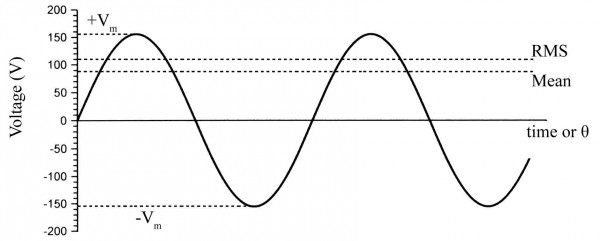
\includegraphics[width=0.8\textwidth]{assets/rms_gemiddelde_sinus.png}
    \caption{De drie waarden op één sinus van $230$~V. De piek ligt op $\pm 325$~V, de effectieve
        waarde (RMS) op $230$~V en de gemiddelde gelijkgerichte waarde (Mean) op $207$~V. Merk op hoe
        dicht RMS en Mean bij elkaar liggen --- precies daarom valt het niet op wanneer een goedkope
        meter de verkeerde van de twee toont.}
    \label{fig:rms-mean-sinus}
\end{figure}
\FloatBarrier

\textbf{Waarom juist de RMS-waarde?} Omdat die het \emph{warmte-effect} vastlegt. De effectieve
waarde van een wisselstroom is per definitie de gelijkstroom die in dezelfde weerstand evenveel
warmte zou produceren. Reken je de warmte over één periode uit:
\[Q_{\text{DC}} = \int_0^T R I^2\,dt = R I^2 T
    \qquad\text{en}\qquad
    Q_{\text{AC}} = \int_0^T R\,i^2(t)\,dt = R\,I_m^2 \int_0^T \sin^2(\omega t)\,dt = R\,\frac{I_m^2}{2}\,T\]
Beide gelijkstellen geeft $I^2 = I_m^2/2$, dus $I = I_m/\sqrt2$. Vandaar de vertrouwde factor
$\sqrt2$, en vandaar ook dat je met effectieve waarden gewoon $P = I^2R$ mag schrijven alsof het
gelijkstroom was.

\frm{Effectieve waarde (RMS)}{A_{\text{eff}} = \sqrt{\frac{1}{T}\int_0^T a^2(t)\,dt}
    \;\;\overset{\text{sinus}}{=}\;\; \frac{A_m}{\sqrt2} \approx 0{,}707\,A_m}
{Met $A_{\text{eff}}$ de effectieve waarde, $a(t)$ het momentane signaal en $T$ de periode in s.
    RMS staat voor \emph{Root Mean Square}: eerst kwadrateren, dan middelen, dan de wortel.
    De rechtse gelijkheid geldt \textbf{alleen} voor een zuivere sinus.}

\frm{$A_{\text{gem}}$}{A_{\text{gem}} = \frac{1}{T/2} \int_0^{T/2} A(t)\,dt = \frac{2 A_m}{\pi} \approx 0{,}637\,A_m}{Met $A_{\text{gem}}$ de gemiddelde gelijkgerichte waarde over een halve periode $T/2$.}

De afleiding daarvan, met $a(t) = A_m \sin(\omega t)$:
\[A_{gem} = \frac{1}{T/2} \int_0^{T/2} A_m \sin(\omega t) dt = \frac{2 A_m}{T} \left[ -\frac{1}{\omega} \cos(\omega t)
        \right]_0^{T/2} = \frac{2 A_m}{T} \cdot \frac{2}{\omega} = \frac{2 A_m}{2\pi / \omega} \cdot \frac{2}{\omega} = \frac{2 A_m}{\pi}\]

\subsubsection{Vormfactor en piekfactor: hoe ``puntig'' is de golf?}

De verhouding tussen die drie waarden hangt alleen van de \emph{vorm} van de golf af, niet van hoe
groot hij is. Twee verhoudingen krijgen een naam.

\frm{Vormfactor en Piekfactor}{k_f = \frac{A_{\text{eff}}}{A_{\text{gem}}} \qquad , \qquad k_p = \frac{A_m}{A_{\text{eff}}}}
{Met $k_f$ de vormfactor ($k_f = 1{,}11$ voor sinus) en $k_p$ de piekfactor of crest factor ($k_p = \sqrt{2} \approx 1{,}414$ voor sinus).}

Lees ze zo:
\begin{itemize}
    \item \textbf{Vormfactor $k_f$} --- hoeveel groter de effectieve waarde is dan het gewone
          gemiddelde. Een blokgolf staat altijd op volle waarde, dus daar zijn beide gelijk en is
          $k_f = 1$. Hoe puntiger de golf, hoe hoger $k_f$.
    \item \textbf{Piekfactor $k_p$} --- hoeveel hoger de piek uitsteekt boven de effectieve waarde.
          Dit is wat een versterker of een voeding moet kunnen slikken zonder te klippen.
\end{itemize}

Figuur~\ref{fig:golfvormen-kf} laat voor vier golfvormen zien waar $A_m$, $A_{\text{eff}}$ en
$A_{\text{gem}}$ liggen. Je ziet meteen waarom de getallen in de tabel eronder verschillen.

\begin{figure}[htbp]
    \centering
    \begin{tikzpicture}[x=1.0cm, y=1.35cm, font=\small]
        % ---------- hulpmacro-achtige opzet: vier panelen ----------
        % paneel 1: zuivere sinus
        \begin{scope}[shift={(0,0)}]
            \draw[->, gray] (-0.2,0) -- (4.5,0) node[right, font=\scriptsize, black] {$\omega t$};
            \draw[->, gray] (0,-1.25) -- (0,1.35);
            \draw[ultra thick, schoolBlue] plot[domain=0:4, samples=80] (\x, {sin(\x*90)});
            \draw[dashed, schoolRed] (0,0.707) -- (4.3,0.707) node[right, font=\scriptsize, schoolRed] {$A_{\text{eff}}$};
            \draw[dashed, schoolGreen!60!black] (0,0.637) -- (3.6,0.637);
            \node[font=\scriptsize, schoolGreen!50!black, right] at (3.6,0.45) {$A_{\text{gem}}$};
            \draw[dotted, gray] (0,1) -- (4.3,1) node[right, font=\scriptsize, black] {$A_m$};
            \node[font=\scriptsize\bfseries, anchor=north] at (2.2,-1.3) {zuivere sinus};
        \end{scope}
        % paneel 2: enkelzijdig gelijkgericht
        \begin{scope}[shift={(7.2,0)}]
            \draw[->, gray] (-0.2,0) -- (4.5,0) node[right, font=\scriptsize, black] {$\omega t$};
            \draw[->, gray] (0,-1.25) -- (0,1.35);
            \draw[ultra thick, schoolBlue] plot[domain=0:2, samples=40] (\x, {sin(\x*90)});
            \draw[ultra thick, schoolBlue] (2,0) -- (4,0);
            \draw[dashed, schoolRed] (0,0.5) -- (4.3,0.5) node[right, font=\scriptsize, schoolRed] {$A_{\text{eff}}$};
            \draw[dashed, schoolGreen!60!black] (0,0.318) -- (3.6,0.318);
            \node[font=\scriptsize, schoolGreen!50!black, right] at (3.6,0.20) {$A_{\text{gem}}$};
            \draw[dotted, gray] (0,1) -- (4.3,1) node[right, font=\scriptsize, black] {$A_m$};
            \node[font=\scriptsize\bfseries, anchor=north, align=center] at (2.2,-1.3) {enkelzijdig\\gelijkgerichte sinus};
        \end{scope}
    \end{tikzpicture}

    \vspace{7mm}

    \begin{tikzpicture}[x=1.0cm, y=1.35cm, font=\small]
        % paneel 3: blokgolf
        \begin{scope}[shift={(0,0)}]
            \draw[->, gray] (-0.2,0) -- (4.5,0) node[right, font=\scriptsize, black] {$\omega t$};
            \draw[->, gray] (0,-1.25) -- (0,1.35);
            \draw[ultra thick, schoolBlue] (0,1) -- (2,1) -- (2,-1) -- (4,-1);
            \draw[dashed, schoolRed] (0,1) -- (4.3,1);
            \node[font=\scriptsize, anchor=west, align=left] at (4.35,1)
            {\textcolor{schoolRed}{$A_{\text{eff}}$} $=$ \textcolor{schoolGreen!50!black}{$A_{\text{gem}}$} $= A_m$};
            \node[font=\scriptsize\bfseries, anchor=north] at (2.2,-1.3) {blokgolf};
        \end{scope}
        % paneel 4: driehoek
        \begin{scope}[shift={(7.2,0)}]
            \draw[->, gray] (-0.2,0) -- (4.5,0) node[right, font=\scriptsize, black] {$\omega t$};
            \draw[->, gray] (0,-1.25) -- (0,1.35);
            \draw[ultra thick, schoolBlue] (0,0) -- (1,1) -- (3,-1) -- (4,0);
            \draw[dashed, schoolRed] (0,0.577) -- (4.3,0.577) node[right, font=\scriptsize, schoolRed] {$A_{\text{eff}}$};
            \draw[dashed, schoolGreen!60!black] (0,0.5) -- (3.6,0.5);
            \node[font=\scriptsize, schoolGreen!50!black, right] at (3.6,0.32) {$A_{\text{gem}}$};
            \draw[dotted, gray] (0,1) -- (4.3,1) node[right, font=\scriptsize, black] {$A_m$};
            \node[font=\scriptsize\bfseries, anchor=north] at (2.2,-1.3) {driehoeksgolf};
        \end{scope}
    \end{tikzpicture}
    \caption{Vier golfvormen met dezelfde piekwaarde $A_m$. De rode lijn is de effectieve waarde, de
        groene het gelijkgerichte gemiddelde. Hoe puntiger de golf, hoe verder beide onder de piek
        zakken --- en hoe verder ze van elkaar af komen te liggen.}
    \label{fig:golfvormen-kf}
\end{figure}
\FloatBarrier

\begin{center}
    \begin{tabular}{@{}lcccc@{}}
        \toprule
        \textbf{Golfvorm}                & $A_{\text{eff}}$          & $A_{\text{gem}}$        & $k_f$                             & $k_p$                       \\
        \midrule
        Zuivere sinus                    & $A_m/\sqrt2 = 0{,}707A_m$ & $2A_m/\pi = 0{,}637A_m$ & $\pi/(2\sqrt2) = \mathbf{1{,}11}$ & $\sqrt2 = \mathbf{1{,}414}$ \\
        Enkelzijdig gelijkgerichte sinus & $A_m/2 = 0{,}5A_m$        & $A_m/\pi = 0{,}318A_m$  & $\pi/2 = \mathbf{1{,}57}$         & $\mathbf{2}$                \\
        Blokgolf                         & $A_m$                     & $A_m$                   & $\mathbf{1{,}0}$                  & $\mathbf{1{,}0}$            \\
        Driehoeksgolf / zaagtand         & $A_m/\sqrt3 = 0{,}577A_m$ & $A_m/2 = 0{,}5A_m$      & $2/\sqrt3 = \mathbf{1{,}155}$     & $\sqrt3 = \mathbf{1{,}732}$ \\
        \bottomrule
    \end{tabular}
\end{center}

\subsubsection{Werking van meetinstrumenten}

Niet elk meettoestel meet hetzelfde bij een niet-sinusvormig signaal:
\begin{itemize}
    \item \textbf{Klassieke draaispoelmeter met gelijkrichter:} meet mechanisch de \textbf{gemiddelde gelijkgerichte waarde} $A_{\text{gem}}$ en vermenigvuldigt die intern met de vaste factor $\mathbf{1{,}11}$ (de vormfactor van een zuivere sinus). Bij een afwijkende golfvorm (bv.\ dimmer, gelijkrichter) wijst dit toestel dus een \emph{foutieve} effectieve waarde aan!
    \item \textbf{Draai-ijzer- / weekijzermeter:} de mechanische afbuiging is evenredig met het kwadraat van de stroom ($i^2$). Hierdoor meet het toestel rechtstreeks de \textbf{echte effectieve waarde} $A_{\text{eff}}$, onafhankelijk van de golfvorm (voor lage netfrequenties).
    \item \textbf{True RMS digitale meter:} bemonstert het signaal digitaal met hoge frequentie en berekent numeriek $\sqrt{\frac{1}{T}\int_0^T a^2(t)\,dt}$. Geeft altijd de correcte effectieve waarde.
\end{itemize}

\begin{wrapfigure}{r}{0.36\textwidth}
    \vspace{-4mm}
    \centering
    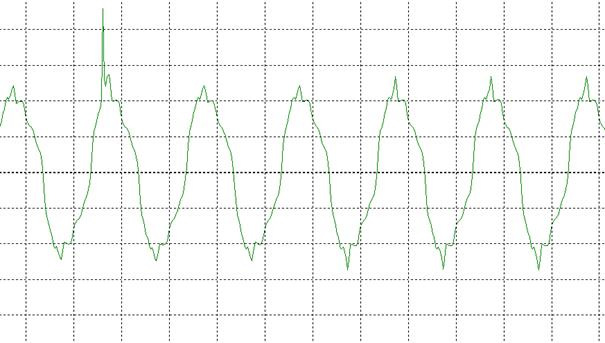
\includegraphics[width=0.34\textwidth]{assets/vervormd_signaal_meter.png}
    \caption{Een vervormd netsignaal. Voor zo'n golf klopt de vaste factor $1{,}11$ niet meer.}
    \label{fig:vervormd-signaal}
    \vspace{-3mm}
\end{wrapfigure}

Dat verschil is geen theorie. De goedkope meter meet $A_{\text{gem}}$ en toont
$A_{\text{gem}} \times 1{,}11$ --- hij \emph{gokt} dat je golf een zuivere sinus is. Hangt er een
dimmer, een schakelende voeding of een frequentieregelaar aan, dan is de golf vervormd
(figuur~\ref{fig:vervormd-signaal}), is de echte vormfactor niet meer $1{,}11$, en klopt de
aflezing gewoon niet. Op een toestel dat het wél goed doet staat daarom expliciet
\textbf{TRUE RMS} gedrukt.

\begin{examenbox}[Reken de vormfactor zelf uit]
    Slide-oefening 4.1.4 doet precies dit: je meet dezelfde vervormde stroom met een
    draaispoelmeter (leest $A_{\text{gem}}$) en met een TRUE RMS-meter (leest $A_{\text{eff}}$), en
    de vormfactor volgt uit de verhouding van de twee aflezingen. Krijg je iets anders dan
    $1{,}11$, dan wéét je dat het signaal geen zuivere sinus is.
\end{examenbox}

\vspace{0.3cm}

\subsection{Fasors}

Een wisselstroom of -spanning kan je ook voorstellen als een roterende vector in het complexe vlak.
Die roterende vector heet een \textbf{sinor}:
\[v(t) = V_m\,e^{j(\omega t + \phi)}\]
Hij draait met $\omega$ rond de oorsprong, en zijn projectie op een as is precies de sinus waarmee je
begon.

Een \keyterm{fasor} is die sinor \textbf{bevroren op $t = 0$}:
\[\underline{V} = V_m\,e^{j\phi} = V_m\angle\phi\]
De tijdsafhankelijkheid $e^{j\omega t}$ laat je gewoon weg. Dat mag, omdat \emph{alle} grootheden in
\'e\'en oefening dezelfde $\omega$ hebben en dus even snel draaien: hun onderlinge hoeken liggen vast.
Precies daarom mag je fasoren nooit optellen als de frequenties verschillen --- dan draaien ze niet
meer synchroon en heeft ``de hoek ertussen'' geen betekenis meer.

\vspace{0.5cm}

\begin{figure}[htbp]
    \centering
    \begin{tikzpicture}[scale=1.25, >=latex]
        % assen
        \draw[->, thick] (-1.0,0) -- (3.5,0) node[right] {Re};
        \draw[->, thick] (0,-0.8) -- (0,3.0) node[above] {Im};

        % projecties
        \coordinate (P) at (1.99,1.67);
        \draw[dashed, gray!70] (P) -- (1.99,0);
        \draw[dashed, gray!70] (P) -- (0,1.67);

        % de fasor zelf
        \draw[->, very thick, schoolBlue] (0,0) -- (P);
        \node[schoolBlue, font=\small, rotate=40, anchor=south] at (1.0,0.84) {lengte $= V_m$};

        % hoek
        \draw[schoolRed, thick] (0.8,0) arc (0:40:0.8);
        \node[schoolRed] at (1.08,0.30) {$\phi$};

        % labels
        \node[schoolBlue, anchor=south west, font=\small] at (2.06,1.70) {$\vec{V} = V_m\angle\phi$};
        \node[anchor=north, font=\scriptsize, align=center] at (1.99,-0.10)
             {$V_m\cos\phi$\\re\"eel deel};
        \node[anchor=east, font=\scriptsize, align=right] at (-0.10,1.67)
             {$V_m\sin\phi$\\imaginair deel};

        % rotatiehint
        \draw[->, thick, schoolGreen!60!black] (2.30,1.93) arc (40:72:3.0);
        \node[schoolGreen!50!black, font=\scriptsize, anchor=west] at (1.35,2.75) {draait met $\omega$};
    \end{tikzpicture}
    \caption{Een fasor in het complexe vlak. De \emph{lengte} van de pijl is de amplitude $V_m$, de
        \emph{hoek} met de re\"ele as is de fasehoek $\phi$. Het re\"ele deel is $V_m\cos\phi$, het
        imaginaire deel $V_m\sin\phi$. In werkelijkheid draait de pijl rond met $\omega$, maar omdat
        \emph{alle} fasoren in een oefening even snel draaien, tekenen we hem stil: alleen de
        onderlinge hoeken doen ertoe.}
    \label{fig:fasor}
\end{figure}
\FloatBarrier

Bij een fasor gaan we de pulsatie $\omega$ niet meer expliciet noteren.
Als je een oefening voor het omzetten van fasor naar tijdsfunctie of omgekeerd doet,
ga je de pulsatie gegeven krijgen.

Je kunt die allemaal doen met je niet-grafische rekenmachine door de modus op
\textbf{complex} $a + jb$ of \textbf{polar} $A_m \angle \phi$ te zetten.

\frm{fasor}{\vec{A} = A_m \angle \phi = A_m (\cos\phi + j \sin\phi) =A_m e^{j\phi}}{Met $\vec{A}$ de fasor van de wisselgrootte A,
    $A_m$ de amplitude (piekwaarde) en $\phi$ de fasehoek in graden of radialen. Het reële deel is $A_m \cos\phi$
    en het imaginaire deel is $A_m \sin\phi$. }

\[A_m = \sqrt{(\text{Re}(\vec{A}))^2 + (\text{Im}(\vec{A}))^2}\]
\[\phi = \tan^{-1}\left(\frac{\text{Im}(\vec{A})}{\text{Re}(\vec{A})}\right)\]

\begin{waarschuwing}[Twee voorwaarden voor je fasoren optelt]
    \textbf{Dezelfde golfvorm.} Alle termen moeten sinus zijn, of allemaal cosinus. Zet om met:
    \[\sin\theta = \cos(\theta - 90^\circ) \qquad\qquad \cos\theta = \sin(\theta + 90^\circ)\]
    $5\cos(3t+7^\circ) + 2\sin(3t-28^\circ)$ mag je dus \textbf{niet} rechtstreeks als
    $5\angle 7^\circ + 2\angle -28^\circ$ schrijven.
    \emph{Dit was letterlijk theorievraag 1 op 20/01/2024 én 22/08/2024.}

    \textbf{Dezelfde frequentie.} Fasoren met een verschillende $\omega$ draaien niet even snel,
    dus hun onderlinge hoek ligt niet vast. Heb je meerdere bronnen met verschillende frequenties,
    reken dan elke bron apart uit bij zijn eigen $\omega$ (superpositie) en tel de resultaten pas
    op in het \emph{tijdsdomein}.
\end{waarschuwing}

\begin{examenbox}[Amplitude of effectieve waarde?]
    Een fasor kan je met de \textbf{amplitude} $A_m$ of met de \textbf{effectieve waarde} / RMS-waarde $A_{\text{eff}}$.

    $A_{\text{eff}} = A_m/\sqrt{2}$ schrijven. Beide mag, zolang je \textbf{consequent} bent.

    Let op waar je welke nodig hebt:
    \begin{itemize}
        \item \textbf{Vermogens} ($P$, $Q$, $S$) reken je altijd met \textbf{effectieve} waarden.
        \item Het \textbf{ogenblikkelijk vermogen} $p(t) = v(t)i(t)$ reken je met de
              \textbf{tijdsfuncties}, dus met piekwaarden.
        \item Meettoestellen (ampèremeters, voltmeters) geven \textbf{effectieve} waarden. ``230~V''
              op een typeplaatje is dus altijd effectief.
    \end{itemize}
\end{examenbox}


\textbf{Voorbeeld:} Alle notaties voor de functie $v(t) = 220 \sin(314t + 30^\circ)$

\[V_m = 220 V\]
\[\omega = 314 \text{ rad/s}\]
\[\phi = 30^\circ = \frac{\pi}{6} \text{ rad}\]

\[a = 220V \cdot \cos(30^\circ) = 190.5 V\]
\[b = 220V \cdot \sin(30^\circ) = 110 V\]
\[\vec{V} = 220 \angle 30^\circ = 220 (\cos 30^\circ + j \sin 30^\circ) =
    220 \left(\frac{\sqrt{3}}{2} + j \cdot \frac{1}{2}\right) = 190.5 + j 110 V\]


\begin{oefening}[Gemiddelde en effectieve stroom]
    \begin{center}
        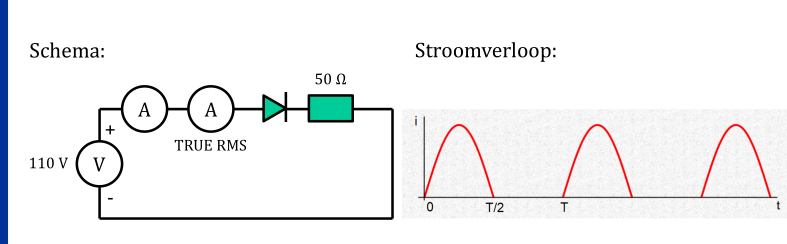
\includegraphics[width=0.8\textwidth]{assets/RMS berekenen .png}
        \captionof{figure}{RMS berekenen}
        \label{fig:RMS berekenen}
    \end{center}

    Een bron van $110\,\text{V}$ (effectieve waarde) voedt een serieschakeling van een diode en een
    weerstand van $50\,\Omega$. De diode laat enkel de positieve helft van de sinus door (enkelzijdige
    gelijkrichting), waardoor de stroom $i(t)$ een halve sinus is die om de periode $T$ herhaalt.
    In de kring staat zowel een gewone (draaispoel-)ampèremeter als een \textit{true RMS}-ampèremeter.

    \vspace{0.3cm}

    Eerst de piekstroom uit de wet van Ohm, met $V_m = \sqrt{2} \cdot V_{\text{eff}}$:
    \[I_m = \frac{V_m}{R} = \frac{\sqrt{2} \cdot 110}{50} = 3.11 \text{ A}\]

    De stroom door de weerstand is dus:
    \[i(t) = 3.11 \sin(\omega t) \quad \text{als} \quad 0 \leq t \leq \frac{T}{2}\]
    \[i(t) = 0 \quad \text{als} \quad \frac{T}{2} \leq t \leq T\]

    \vspace{0.3cm}

    \[I_{gem} = 0.64 \cdot I_m = 1.98 \text{ A} \quad \text{over halve periode (sinus)}\]
    \[= 0.99 \text{ A} \quad \text{over hele periode}\]

    aflezing op draaispoelmeter: \quad $I_{gem} \cdot 1.11 = \underline{1,10 \text{ A}}$
    \hfill \small (vormfactor sinus)

    \vspace{0.3cm}

    Voor deze stroom:
    \[I_{eff} = \sqrt{\frac{1}{T}\left(\int_0^{T/2} i^2(t)\,dt + \int_{T/2}^T i^2(t)\,dt\right)} = \frac{1}{\sqrt{2}} \cdot \frac{I_m}{\sqrt{2}} = \frac{I_m}{2}\]

    Voor echte sinus:
    \[I_{eff} = \sqrt{\frac{1}{T}\left(\int_0^{T/2} i^2(t)\,dt + \int_{T/2}^T i^2(t)\,dt\right)} = \sqrt{\frac{2}{T}\int_0^{T/2} i^2(t)\,dt} = \frac{I_m}{\sqrt{2}}\]

    aflezing op TRUE RMS meter: \quad $I_{eff} = \dfrac{I_m}{2} = \dfrac{3.11}{2} = \underline{1{,}56 \text{ A}}$

    vormfactor van de stroom: \quad $\dfrac{I_{eff}}{I_{gem}} = \dfrac{1{,}56}{0{,}99} = 1{,}58$

\end{oefening}

\section{Hoofdstuk 2: Wisselstroom ketens}



Een spoel en een condensator verschuiven de stroom ten opzichte van de spanning, maar in
\emph{tegengestelde} richting. Het klassieke ezelsbruggetje daarvoor is \keyterm{ELI the ICE man},
met $E$ de spanning, $I$ de stroom, $L$ de spoel en $C$ de condensator:

\begin{itemize}
    \item \textbf{ELI} --- bij een spoel ($L$) komt $E$ vóór $I$: de \textbf{spanning ijlt voor} op
          de stroom, of omgekeerd gezegd, de stroom \textbf{ijlt na}. Een spoel is dus
          \textbf{naijlend} (Engels: \emph{lagging}).
    \item \textbf{ICE} --- bij een condensator ($C$) komt $I$ vóór $E$: de \textbf{stroom ijlt voor}
          op de spanning. Een condensator is dus \textbf{voorijlend} (Engels: \emph{leading}).
\end{itemize}

De letters staan dus in de volgorde waarin de grootheden ``aankomen''. Bij beide is de
verschuiving $90^\circ$; een weerstand verschuift niets.

\begin{figure}[htbp]
    \centering
    {\bfseries 1. Zuivere spoel $L$ --- ELI: de spanning ijlt $90^\circ$ v\'o\'or op de stroom.}\par
    \vspace{2mm}
\begin{tikzpicture}[scale=0.86, line cap=round, line join=round]
        % ---- golfvormen ----
        \begin{scope}[shift={(0,0)}]
            \draw[->, thick] (-0.3,0) -- (7.3,0) node[right, font=\footnotesize] {$\omega t$};
            \draw[->, thick] (0,-1.55) -- (0,1.95);
            \node[font=\scriptsize, rotate=90, anchor=south] at (-0.55,0) {$v(t),\ i_L(t)$};

            \foreach \xg in {1.571, 3.142, 4.712, 6.283}
                \draw[gray!30, dotted, thick] (\xg,-1.35) -- (\xg,1.4);

            \node[below, font=\scriptsize] at (1.571, -0.05) {$\tfrac{\pi}{2}$};
            \node[below, font=\scriptsize] at (3.142, -0.05) {$\pi$};
            \node[below, font=\scriptsize] at (4.712, -0.05) {$\tfrac{3\pi}{2}$};
            \node[below, font=\scriptsize] at (6.283, -0.05) {$2\pi$};

            \draw[domain=0:6.6, samples=120, smooth, ultra thick, schoolBlue]
                plot (\x, {1.35*sin(\x r)});
            \draw[domain=0:6.6, samples=120, smooth, ultra thick, schoolRed, dashed]
                plot (\x, {-1.05*cos(\x r)});

            \draw[schoolBlue, fill=schoolBlue] (1.571, 1.35) circle (0.045);
            \draw[schoolRed, fill=schoolRed] (3.142, 1.05) circle (0.045);
            \draw[<->, thick, schoolGreen!60!black] (1.571, 1.62) -- (3.142, 1.62) node[midway, above, font=\scriptsize\bfseries, text=schoolGreen!50!black] {$\Delta\phi = 90^\circ$};

            \draw[ultra thick, schoolBlue] (0.3, -2.05) -- (0.8, -2.05)
                node[right, font=\scriptsize, text=black] {$v(t) = V_m\sin(\omega t)$};
            \draw[ultra thick, schoolRed, dashed] (4.0, -2.05) -- (4.5, -2.05)
                node[right, font=\scriptsize, text=black] {$i_L(t) = I_m\sin(\omega t - 90^\circ)$};
        \end{scope}

        % ---- fasordiagram ----
        \begin{scope}[shift={(9.9,0)}]
            \draw[->, thick] (-1.1,0) -- (2.4,0) node[right, font=\footnotesize] {Re};
            \draw[->, thick] (0,-1.75) -- (0,1.95) node[above, font=\footnotesize] {Im};

            \draw[->, ultra thick, schoolBlue] (0,0) -- (1.8,0)
                node[above, font=\scriptsize\bfseries, yshift=1mm] {$\vec{V} = V\angle 0^\circ$};
            \draw[->, ultra thick, schoolRed] (0,0) -- (0,-1.35)
                node[below right, font=\scriptsize\bfseries] {$\vec{I}_L = I_L\angle -90^\circ$};

            \fill (0,0) circle (0.05);
            \draw[->, thick, schoolGreen!60!black] (0.55,0) arc (0:-90:0.55); \node[schoolGreen!50!black, font=\scriptsize\bfseries] at (0.92, -0.42) {$-90^\circ$};
            \node[font=\scriptsize, align=center, text=gray!80!black] at (1.0, 1.35) {stroom ijlt $90^\circ$ \emph{na}};
        \end{scope}
    \end{tikzpicture}

    \vspace{7mm}

    {\bfseries 2. Zuivere condensator $C$ --- ICE: de stroom ijlt $90^\circ$ v\'o\'or op de spanning.}\par
    \vspace{2mm}
\begin{tikzpicture}[scale=0.86, line cap=round, line join=round]
        % ---- golfvormen ----
        \begin{scope}[shift={(0,0)}]
            \draw[->, thick] (-0.3,0) -- (7.3,0) node[right, font=\footnotesize] {$\omega t$};
            \draw[->, thick] (0,-1.55) -- (0,1.95);
            \node[font=\scriptsize, rotate=90, anchor=south] at (-0.55,0) {$v(t),\ i_C(t)$};

            \foreach \xg in {1.571, 3.142, 4.712, 6.283}
                \draw[gray!30, dotted, thick] (\xg,-1.35) -- (\xg,1.4);

            \node[below, font=\scriptsize] at (1.571, -0.05) {$\tfrac{\pi}{2}$};
            \node[below, font=\scriptsize] at (3.142, -0.05) {$\pi$};
            \node[below, font=\scriptsize] at (4.712, -0.05) {$\tfrac{3\pi}{2}$};
            \node[below, font=\scriptsize] at (6.283, -0.05) {$2\pi$};

            \draw[domain=0:6.6, samples=120, smooth, ultra thick, schoolBlue]
                plot (\x, {1.35*sin(\x r)});
            \draw[domain=0:6.6, samples=120, smooth, ultra thick, schoolRed, dashed]
                plot (\x, {1.05*cos(\x r)});

            \draw[schoolBlue, fill=schoolBlue] (1.571, 1.35) circle (0.045);
            \draw[schoolRed, fill=schoolRed] (0, 1.05) circle (0.045);
            \draw[<->, thick, schoolGreen!60!black] (0, 1.62) -- (1.571, 1.62) node[midway, above, font=\scriptsize\bfseries, text=schoolGreen!50!black] {$\Delta\phi = 90^\circ$};

            \draw[ultra thick, schoolBlue] (0.3, -2.05) -- (0.8, -2.05)
                node[right, font=\scriptsize, text=black] {$v(t) = V_m\sin(\omega t)$};
            \draw[ultra thick, schoolRed, dashed] (4.0, -2.05) -- (4.5, -2.05)
                node[right, font=\scriptsize, text=black] {$i_C(t) = I_m\sin(\omega t + 90^\circ)$};
        \end{scope}

        % ---- fasordiagram ----
        \begin{scope}[shift={(9.9,0)}]
            \draw[->, thick] (-1.1,0) -- (2.4,0) node[right, font=\footnotesize] {Re};
            \draw[->, thick] (0,-1.75) -- (0,1.95) node[above, font=\footnotesize] {Im};

            \draw[->, ultra thick, schoolBlue] (0,0) -- (1.8,0)
                node[below, font=\scriptsize\bfseries, yshift=-1mm] {$\vec{V} = V\angle 0^\circ$};
            \draw[->, ultra thick, schoolRed] (0,0) -- (0,1.35)
                node[above right, font=\scriptsize\bfseries] {$\vec{I}_C = I_C\angle +90^\circ$};

            \fill (0,0) circle (0.05);
            \draw[->, thick, schoolGreen!60!black] (0.55,0) arc (0:90:0.55); \node[schoolGreen!50!black, font=\scriptsize\bfseries] at (0.52, 0.80) {$+90^\circ$};
            \node[font=\scriptsize, align=center, text=gray!80!black] at (1.0, -1.35) {stroom ijlt $90^\circ$ \emph{voor}};
        \end{scope}
    \end{tikzpicture}
    \caption{Faseverschuiving tussen spanning en stroom, links in de tijd en rechts als
        fasordiagramma. Boven (spoel): $v(t)$ bereikt haar maximum $90^\circ$ v\'o\'or $i_L(t)$, dus de
        stroom ijlt na. Onder (condensator): $i_C(t)$ bereikt haar maximum $90^\circ$ v\'o\'or $v(t)$,
        dus de stroom ijlt voor. In het fasordiagramma is dat simpelweg een pijl die $90^\circ$ naar
        beneden of naar boven staat.}
    \label{fig:eli-ice-vergelijking}
\end{figure}
\FloatBarrier

\subsubsection{Impedantie}

\begin{conceptbox}[Impedantie en reactantie]
    De \textbf{impedantie} $\underline{Z}$ is de wisselstroomversie van weerstand: ze zegt hoeveel de
    keten de stroom tegenhoudt \'en hoeveel ze de stroom in de tijd verschuift.

    Het re\"ele deel is de gewone \textbf{weerstand} $R$ (die zet vermogen om in warmte), het
    imaginaire deel is de \textbf{reactantie} $X$ (die zet geen vermogen om, maar slaat energie op in
    een spoel of condensator en geeft ze weer terug):
    \[\underline{Z} = R + jX \qquad [\Omega]\]

    Verwar reactantie niet met \emph{reluctantie}: dat laatste is de magnetische weerstand van een
    ijzeren kern, en heeft niets met dit hoofdstuk te maken.
\end{conceptbox}
\frm{Impedantie}{Z = R + jX}{Met Z de impedantie in Ohm, R de weerstand in Ohm en X de reactantie in Ohm.}

\frm{Reactantie spoel}{X_L = \omega L}{Met $X_L$ de inductieve reactantie in Ohm, $\omega$ de pulsatie in rad/s en L de inductantie in Henry.}
\frm{Reactantie condensator}{X_C = \frac{-1}{\omega C}}{Met $X_C$ de capacitieve reactantie in Ohm, $\omega$ de pulsatie in rad/s en C de capaciteit in Farad.}

\frm{Totale impedantie in serie}{Z_{totaal} = \sqrt{R^2 + (X_L + X_C)^2}}{Met $Z_{totaal}$ de totale impedantie in Ohm, R de weerstand in Ohm, $X_L$ de inductieve reactantie in Ohm en $X_C$ de capacitieve reactantie in Ohm.}

\frm{Hoek van de impedantie}{\tan \phi = \frac{X_L + X_C}{R}}{Met $\phi$ de fasehoek van de impedantie in graden of radialen, R de weerstand in Ohm, $X_L$ de inductieve reactantie in Ohm en $X_C$ de capacitieve reactantie in Ohm.}


\subsection{Vermogen in wisselstroomkringen}

\begin{waarschuwing}[Let op het verschil tussen een fasor en een grootte]
    In dit hoofdstuk staan drie soorten symbolen door elkaar. Ze zijn \textbf{niet} inwisselbaar:
    \begin{itemize}
        \item \textbf{Een onderstreepte letter} ($\underline{V}$, $\underline{I}$, $\underline{S}$,
              $\underline{Z}$) is een \textbf{complex} getal: het heeft een grootte \emph{en} een hoek.
              Hiermee mag je optellen, delen en vermenigvuldigen zoals je gewend bent.
        \item \textbf{Dezelfde letter tussen modulusstrepen} ($|\underline{V}|$, $|\underline{S}|$)
              is alleen de \textbf{grootte}. De hoek is weg, dus je mag hier \emph{niet} mee verder
              rekenen alsof het een fasor is. $|\underline{S}_1| + |\underline{S}_2|$ is bijvoorbeeld
              fout.
        \item \textbf{$P$, $Q$, $R$, $X$ en $\cos\phi$} zijn gewone re\"ele getallen. Die mag je wel
              gewoon optellen, want ze zijn per definitie al een projectie op \'e\'en as.
    \end{itemize}
    Vuistregel: zodra er een hoek in het spel zit, hoort er een streep onder de letter.
\end{waarschuwing}

Omdat de stroom en de spanning oscilleren in tijd, oscilleert
het vermogen ook in tijd.

\begin{figure}[ht]
    \centering
    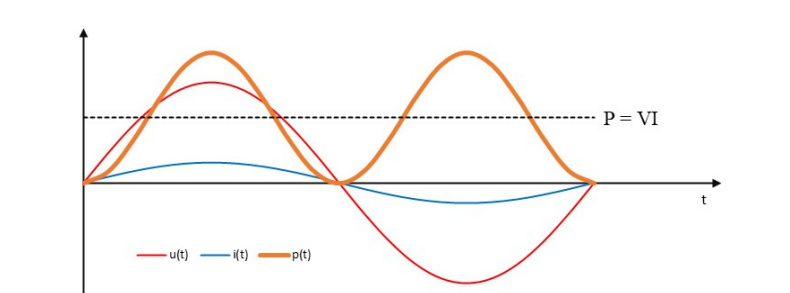
\includegraphics[width=0.8\textwidth]{assets/vermogen.png}
    \caption{Vermogen in functie van tijd.}
    \label{fig:vermogen.png}
\end{figure}

We beginnen met het eenvoudigste geval: een \textbf{zuiver ohmse} $R$ belasting, waarbij spanning
en stroom in fase liggen.

\[p(t) = v(t) \cdot i(t) = V_m \sin(\omega t ) \cdot I_m \sin(\omega t)\]
\[= V_m I_m \sin^2(\omega t)\]
\[\sin^2(x) = \frac{1 - \cos(2x)}{2}\] (uit de goniometrische formules)
\[p(t) = V_m I_m \cdot \frac{1 - \cos(2\omega t)}{2} = \frac{V_m I_m}{2} (1 - \cos(2\omega t))\]

We willen dit uitdrukken in \textbf{effectieve waarden} in plaats van in de piekwaarden $V_m$ en $I_m$,
want dat zijn de waarden die je meet.

\[V_{\text{eff}} = \frac{V_m}{\sqrt{2}} \quad\Longleftrightarrow\quad V_m = \sqrt{2}\,V_{\text{eff}}\]
\[I_{\text{eff}} = \frac{I_m}{\sqrt{2}} \quad\Longleftrightarrow\quad I_m = \sqrt{2}\,I_{\text{eff}}\]
\[\frac{V_m I_m}{2} = \frac{\sqrt{2}\,V_{\text{eff}} \cdot \sqrt{2}\,I_{\text{eff}}}{2} = V_{\text{eff}} I_{\text{eff}}\]

Ingevuld geeft dat:
\[p(t) = V_{\text{eff}} I_{\text{eff}}\left(1 - \cos(2\omega t)\right)\]

Twee dingen vallen op. Het \textbf{gemiddelde} van $p(t)$ is $V_{\text{eff}}I_{\text{eff}}$, want de cosinusterm
heeft gemiddelde nul. En $p(t)$ wordt hier \textbf{nooit negatief}: een weerstand geeft geen
energie terug. Bij een spoel of condensator is dat wél zo, en dat is precies waar $Q$ vandaan komt.

Afhankelijk van het circuit kan het zijn dat de stroom voorloopt of achterloopt op de spanning.

\begin{figure}[ht]
    \centering
    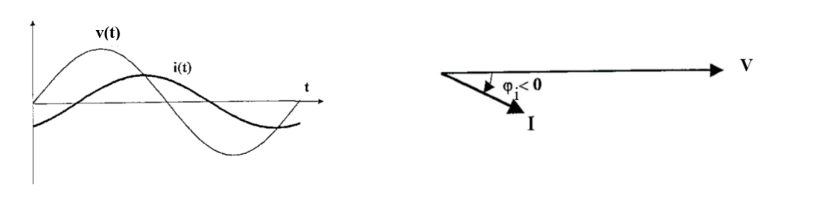
\includegraphics[width=0.8\textwidth]{assets/stroomachtervoltage.png}
    \caption{Stroom die achterloopt op de spanning.}
    \label{fig:stroomachtervoltage.png}
\end{figure}

Welk vermogen wordt er nu verbruikt in het circuit?

Voor een algemene belasting met fasehoek $\phi$ (bv.\ een $RL$- of $RC$-keten) luidt het \textbf{ogenblikkelijk vermogen}:
\[p(t) = v(t) \cdot i(t) = V_m \sin(\omega t) \cdot I_m \sin(\omega t - \phi)\]
\[p(t) = V_{\text{eff}} I_{\text{eff}} \cos\phi \cdot (1 - \cos 2\omega t) + V_{\text{eff}} I_{\text{eff}} \sin\phi \cdot \sin 2\omega t\]
\[\boxed{p(t) = P \cdot (1 - \cos 2\omega t) + Q \cdot \sin 2\omega t}\]

Hierin zien we direct de fysische betekenis van $P$ en $Q$:
\begin{itemize}
    \item Het eerste deel $P(1 - \cos 2\omega t)$ is \textbf{unidirectioneel} (altijd $\ge 0$): dit is het vermogen dat permanent in de ohmse weerstand in warmte of arbeid wordt omgezet (met gemiddelde $P$).
    \item Het tweede deel $Q\sin 2\omega t$ is \textbf{puur oscillerend} met frequentie $2\omega$ en gemiddelde nul: dit vermogen pendelt continu heen en weer tussen bron en het magnetische/elektrische veld van de spoel/condensator.
\end{itemize}

\frm{Actief vermogen}{P = V_{\text{eff}} I_{\text{eff}} \cos \phi}{Met P het actieve vermogen in Watt, $V_{\text{eff}}$ de effectieve spanning in Volt, $I_{\text{eff}}$ de effectieve stroom in
    Ampère en $\phi$ de fasehoek tussen spanning en stroom in graden of radialen.}


Het schijnbaar vermogen is het vermogen dat de bron moet leveren, maar dat niet allemaal nuttig
wordt gebruikt. Het is wat je krijgt als je gewoon de gemeten spanning met de gemeten stroom
vermenigvuldigt, zonder je iets van de fasehoek aan te trekken. Dat is dus een \textbf{grootte},
geen fasor --- vandaar de modulusstrepen.

\frm{Schijnbaar vermogen (grootte)}{|\underline{S}| = V_{\text{eff}} \cdot I_{\text{eff}}}
{Met $|\underline{S}|$ de grootte van het schijnbaar vermogen in Volt-Ampère (VA), $V_{\text{eff}}$
    de effectieve spanning in Volt en $I_{\text{eff}}$ de effectieve stroom in Ampère.
    Dit is de \emph{lengte} van de vermogendriehoek, niet het complexe vermogen zelf.}


Het reactief vermogen is het vermogen dat gebruikt wordt door de spoel of condensator om een magnetisch of elektrisch veld op te bouwen.

Dit vermogen wordt dus niet gebruikt door normale belastingen zoals een lamp of een motor,
maar wordt wel door de bron geleverd. Het is dus een soort van ``verlies'' dat je moet betalen, maar dat je niet nuttig kan gebruiken.


\frm{reactief vermogen}{Q = V_{\text{eff}} I_{\text{eff}} \sin \phi}{Met Q het reactief vermogen in Volt-Ampère reactief (VAR), $V_{\text{eff}}$
    de effectieve spanning in Volt, $I_{\text{eff}}$ de effectieve stroom in Ampère en $\phi$ de fasehoek tussen spanning en stroom in graden of radialen.}

\begin{figure}[htbp]
    \centering
    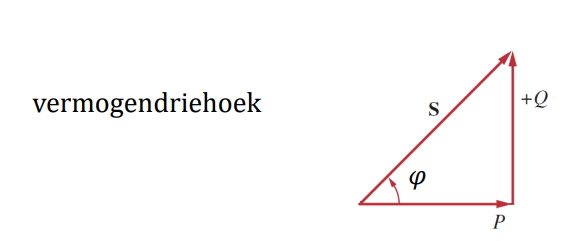
\includegraphics[width=0.6\textwidth]{assets/Vermogendriehoek.png}
    \caption{Vermogendriehoek die de relatie toont tussen actief vermogen P, reactief vermogen Q en schijnbaar vermogen S.}
    \label{fig:Vermogendriehoek.png}
\end{figure}

\frm{Vermogendriehoek}{\underline{S} = P + jQ \qquad\text{met}\qquad |\underline{S}| = \sqrt{P^2 + Q^2}}
{Met $\underline{S}$ het complexe vermogen in VA, $P$ het actieve vermogen in W en $Q$ het reactief
    vermogen in VAR. $P$ is de horizontale zijde, $Q$ de verticale, $|\underline{S}|$ de schuine zijde.}

Omdat het een rechthoekige driehoek is, ligt de fasehoek meteen vast zodra je $P$ en $Q$ kent. Je
hebt de spanning en de stroom er dan niet meer bij nodig:

\frm{Fasehoek uit $P$ en $Q$}{\tan\phi = \frac{Q}{P} \qquad\Longrightarrow\qquad \phi = \arctan\!\left(\frac{Q}{P}\right)}
{Met $\phi$ de fasehoek tussen spanning en stroom. Let op de volgorde: $Q$ staat \textbf{boven},
    $P$ onder --- de overstaande zijde gedeeld door de aanliggende. Het teken van $Q$ geeft meteen ook
    het teken van $\phi$: $Q > 0$ is inductief (naijlend), $Q < 0$ capacitief (voorijlend).}

\frm{Arbeidsfactor}{\text{arbeidsfactor} = \cos \phi = \frac{P}{|\underline{S}|} = \frac{P}{\sqrt{P^2+Q^2}}}
{De verhouding tussen het actieve vermogen $P$ en de grootte van het schijnbaar vermogen
    $|\underline{S}|$. Het geeft aan welk deel van wat de bron levert daadwerkelijk nuttig werk wordt.}

\subsubsection{Complex vermogen}

De drie vermogens hierboven bereken je het snelst in één keer, als \keyterm{complex vermogen}.

\frm{Complex vermogen}{\underline{S} = \underline{V} \cdot \underline{I}^{*} = P + jQ}
{Met $\underline{S}$ het complex vermogen in VA, $\underline{V}$ de spanningsfasor in V,
    $\underline{I}^{*}$ de \emph{complex toegevoegde} van de stroomfasor in A, $P$ het actief
    vermogen in W en $Q$ het reactief vermogen in VAR. Werk je met effectieve waarden in de fasoren,
    dan komt $\underline{S}$ er meteen goed uit; werk je met piekwaarden, dan moet er nog een factor
    $\tfrac12$ voor.}

\textbf{Waar komt dat vandaan?} Neem de spanningsfasor en de stroomfasor in effectieve waarden:
\[\underline{V} = V_{\text{eff}}\angle\phi_V \qquad\qquad \underline{I} = I_{\text{eff}}\angle\phi_I\]

\stapreden{Neem de complex toegevoegde van de stroom. Dat keert alleen het teken van de hoek om:}
\[\underline{I}^{*} = I_{\text{eff}}\angle(-\phi_I)\]

\stapreden{Vermenigvuldig. Bij een product in polaire vorm vermenigvuldig je de groottes en tel je de hoeken op:}
\[\underline{S} = \underline{V}\,\underline{I}^{*}
    = V_{\text{eff}} I_{\text{eff}} \,\angle\,(\phi_V - \phi_I)
    = V_{\text{eff}} I_{\text{eff}} \,\angle\,\phi\]

\stapreden{De grootte van dit product is precies het schijnbaar vermogen, en de hoek is precies de faseverschuiving tussen spanning en stroom:}
\[|\underline{S}| = V_{\text{eff}} I_{\text{eff}} \qquad\qquad \arg(\underline{S}) = \phi = \phi_V - \phi_I\]

\stapreden{Schrijf hetzelfde getal nu in rechthoekige vorm:}
\[\underline{S} = |\underline{S}|\cos\phi + j\,|\underline{S}|\sin\phi
    = \underbrace{V_{\text{eff}} I_{\text{eff}}\cos\phi}_{P}
    \;+\; j\,\underbrace{V_{\text{eff}} I_{\text{eff}}\sin\phi}_{Q}
    \;=\; P + jQ\]

Daarmee klopt de cirkel: $P = V_{\text{eff}} I_{\text{eff}}\cos\phi$ en
$Q = V_{\text{eff}} I_{\text{eff}}\sin\phi$ zijn geen aparte definities die je uit het hoofd moet
leren, het zijn gewoon het re\"ele en het imaginaire deel van hetzelfde complexe getal
$\underline{S}$. En $|\underline{S}| = V_{\text{eff}} I_{\text{eff}}$ is de \emph{lengte} ervan ---
dus zonder hoek, en dus niet zomaar optelbaar met een ander schijnbaar vermogen.

Waarom die complex toegevoegde? Je wil de hoek \emph{tussen} $\underline{V}$ en
$\underline{I}$, dus $\phi = \phi_V - \phi_I$. Bij een gewone vermenigvuldiging tellen de hoeken
op ($\phi_V + \phi_I$), en dat is niet wat je zoekt. Door de toegevoegde te nemen keer je het teken
van $\phi_I$ om, en dan geeft de vermenigvuldiging precies $\phi_V - \phi_I$. Vergeet je de ster,
dan krijg je een verkeerde $\phi$ en dus een verkeerde $P$ en $Q$.

\begin{examenbox}[Meerdere belastingen samen]
    Hangen er meerdere belastingen op dezelfde bron, dan tel je \textbf{$P$ en $Q$ apart} op:
    \[P_T = P_1 + P_2 + \dots \qquad Q_T = Q_1 + Q_2 + \dots \qquad \underline{S}_T = P_T + jQ_T\]
    \[\cos\phi_T = \frac{P_T}{|\underline{S}_T|} = \frac{P_T}{\sqrt{P_T^2 + Q_T^2}}\]
    \belangrijk{Twee klassieke fouten:} $|\underline{S}_T| \neq |S_1| + |S_2|$, en
    $\cos\phi_T$ is \textbf{niet} het gemiddelde van de arbeidsfactoren. Schijnbare vermogens
    zijn vectoren; alleen $P$ en $Q$ zijn scalair optelbaar.
\end{examenbox}

Het teken van $Q$ vertelt je meteen wat voor last je hebt:
\begin{itemize}
    \item $Q > 0$: \textbf{inductief} (naijlend), de stroom loopt achter op de spanning;
    \item $Q < 0$: \textbf{capacitief} (voorijlend), de stroom loopt voor op de spanning;
    \item $Q = 0$: zuiver ohms, of de keten is in resonantie.
\end{itemize}

\subsubsection{Vermogen rechtstreeks uit stroom en impedantie}

Ken je de stroom door een tak en de impedantie ervan, dan hoef je de spanning niet eens te
berekenen:

\frm{Vermogen per tak}{P = I^2 R \quad , \quad Q = I^2 X}
{Met $P$ het actief vermogen in W, $Q$ het reactief vermogen in VAR, $I$ de effectieve stroom door
    de tak in A, $R$ het reële deel en $X$ het imaginaire deel van de takimpedantie in $\Omega$.}

Dit is vaak de \textbf{snelste} weg bij ongebalanceerde 3-fase oefeningen: je berekent per tak de
fasestroom en telt daarna gewoon alle $I^2R$ en $I^2X$ op.

\begin{examenbox}[Eindcontrole die je altijd moet doen]
    Alleen \textbf{weerstanden} verbruiken actief vermogen. Spoelen en condensatoren slaan
    energie op en geven ze weer af, dus hun gemiddeld actief vermogen is nul. Daarom moet altijd
    gelden:
    \[P_{\text{bron}} = \sum_{\text{takken}} I^2 R\]
    Klopt dat niet, dan zit er ergens een rekenfout. Dit kost je tien seconden en redt je oefening.
\end{examenbox}

\begin{oefening}[Voorbeeldberekening: Vermogens en impedantie]
    \textbf{Opgave:} Gegeven $\underline{V} = 110\angle 85^\circ\text{ V}$ en $\underline{I} = 0{,}4\angle 15^\circ\text{ A}$. Bepaal $S, P, Q, \cos\phi$ en $\underline{Z}$.

    \textbf{Oplossing:}

    Eerst het faseverschil, want daar hangt al de rest van af:
    \[\phi = \phi_V - \phi_I = 85^\circ - 15^\circ = 70^\circ \qquad (\text{stroom ijlt na, dus inductief})\]

    Het schijnbaar vermogen is gewoon het product van de twee groottes:
    \[|\underline{S}| = V_{\text{eff}} \cdot I_{\text{eff}} = 110 \cdot 0{,}4 = \mathbf{44}\ \text{VA}\]

    Actief en reactief vermogen zijn de projecties daarvan:
    \[P = |\underline{S}| \cos\phi = 44 \cdot 0{,}342 = \mathbf{15{,}05}\ \text{W}\]
    \[Q = |\underline{S}| \sin\phi = 44 \cdot 0{,}9397 = \mathbf{41{,}35}\ \text{VAR} \qquad (\text{inductief})\]

    De arbeidsfactor volgt uit dezelfde driehoek:
    \[\cos\phi = \frac{P}{|\underline{S}|} = \frac{15{,}05}{44} = \mathbf{0{,}342} \qquad (\text{naijlend})\]

    En de impedantie is de deling van de twee fasoren:
    \[\underline{Z} = \frac{\underline{V}}{\underline{I}}
        = \frac{110\angle 85^\circ}{0{,}4\angle 15^\circ}
        = \mathbf{275\angle 70^\circ}\ \Omega
        = 94{,}06 + j258{,}4\ \Omega\]
\end{oefening}

\begin{examenbox}[Geometrie in het fasordiagram]
    In veel examenoefeningen zijn de fasoren niet rechtstreeks via algebraïsche formules gegeven, maar via gemeten lengtes (ampèremeters) of spanningen. De ontbrekende hoeken los je dan direct op met de goniometrische driehoeksregels:
\end{examenbox}

\frm{Cosinusregel}{c^2 = a^2 + b^2 - 2ab \cos \theta}{Met $a, b, c$ de zijden van de fasordriehoek en $\theta$ de overstaande hoek van $c$.}
\frm{Sinusregel}{\frac{a}{\sin A} = \frac{b}{\sin B} = \frac{c}{\sin C}}{Met $A, B, C$ de hoeken tegenover de respectievelijke zijden $a, b, c$.}

\begin{figure}[H]
    \centering
    \begin{tikzpicture}[scale=1.3, line cap=round, line join=round]
        % Vertices (scalene triangle)
        \coordinate (A) at (0,0);
        \coordinate (B) at (4.0,0);
        \coordinate (C) at (1.3,2.4);

        % Triangle
        \draw[thick] (A) -- (B) -- (C) -- cycle;
        \fill (A) circle (0.03);
        \fill (B) circle (0.03);
        \fill (C) circle (0.03);

        % Vertex labels
        \node[red, font=\small, below left]  at (A) {$A$};
        \node[red, font=\small, below right] at (B) {$B$};
        \node[red, font=\small, above]      at (C) {$C$};

        % Side labels (a opposite A, b opposite B, c opposite C)
        \path (B) -- (C) node[midway, right,  font=\small, text=blue] {$a$};
        \path (A) -- (C) node[midway, left,   font=\small, text=blue] {$b$};
        \path (A) -- (B) node[midway, below,  font=\small, text=blue] {$c$};

        % Angle marker at C (theta)
        \pic[draw=red, angle radius=7mm, angle eccentricity=1.25] {angle = A--C--B};
        \node[red, font=\small] at ($(C)+(0.1,-0.28)$) {$\theta$};
    \end{tikzpicture}
    \caption{Driehoek met zijden $a$, $b$, $c$ tegenover hoeken $A$, $B$, $C$. Voor de cosinusregel geldt (met $\theta = \angle C$): $c^2 = a^2 + b^2 - 2ab\cos\theta$. De sinusregel: $\frac{a}{\sin A} = \frac{b}{\sin B} = \frac{c}{\sin C}$.}
    \label{fig:triangle-rules}
\end{figure}
\FloatBarrier

\subsection{Arbeidsfactorcorrectie}

Een installatie met veel motoren heeft een slechte $\cos\phi$: ze trekt veel reactief vermogen.
Dat vermogen doet geen nuttig werk, maar moet wél door de kabels getransporteerd worden. Daardoor
is de stroom groter dan nodig, en dus ook het $I^2R$-verlies in het net.

\textbf{De oplossing:} zet een condensator parallel over de installatie. Die levert het reactief
vermogen \emph{ter plaatse}, zodat het net het niet meer moet aanvoeren.

\begin{figure}[ht]
    \centering
    \begin{tikzpicture}[scale=1.0, line width=0.8pt]
        \draw[->, thick] (0,0) -- (6.6,0) node[right, font=\small] {$P$};
        \draw[->, thick] (0,0) -- (0,3.6) node[above, font=\small] {$Q$};
        % oude driehoek
        \draw[schoolRed, very thick] (0,0) -- (4.6,0) -- (4.6,3.0) -- cycle;
        \node[schoolRed, font=\small] at (2.2,1.9) {$S$};
        \node[schoolRed, font=\small] at (5.0,1.6) {$Q$};
        % nieuwe driehoek
        \draw[schoolGreen, very thick] (0,0) -- (4.6,0) -- (4.6,1.1) -- cycle;
        \node[schoolGreen, font=\small] at (2.4,0.35) {$S'$};
        \node[schoolGreen, font=\small] at (5.0,0.55) {$Q'$};
        % Qc
        \draw[<->, schoolBlue, very thick] (4.15,1.1) -- (4.15,3.0);
        \node[schoolBlue, font=\small] at (3.75,2.05) {$Q_C$};
        % hoeken
        \node[font=\scriptsize] at (0.95,0.62) {$\phi_1$};
        \node[font=\scriptsize] at (1.25,0.15) {$\phi_2$};
        \node[font=\small] at (2.3,-0.35) {$P$ blijft gelijk};
    \end{tikzpicture}
    \caption{Arbeidsfactorcorrectie. Het actief vermogen $P$ verandert niet; de condensator duwt
        alleen $Q$ omlaag, waardoor $S$ (en dus de stroom) kleiner wordt.}
    \label{fig:pf-correctie}
\end{figure}
\FloatBarrier

\frm{Reactief vermogen van de condensator}{|Q_C| = P\left(\tan|\phi_1| - \tan|\phi_2|\right)}
{Met $|Q_C|$ het reactief vermogen dat de condensator moet leveren in VAR, $P$ het actief vermogen
    van de installatie in W, $\phi_1$ de huidige fasehoek en $\phi_2$ de gewenste fasehoek.}

\textbf{Waar die formule vandaan komt.} Lees ze rechtstreeks af van de twee driehoeken in
figuur~\ref{fig:pf-correctie}, die dezelfde horizontale zijde $P$ delen.

\stapreden{In elke rechthoekige vermogendriehoek is $Q$ de overstaande zijde en $P$ de aanliggende:}
\[\tan\phi = \frac{Q}{P} \qquad\Longrightarrow\qquad Q = P\tan\phi\]

\stapreden{Dat geldt zowel vóór als na de correctie, en $P$ verandert niet (een condensator zet geen actief vermogen om):}
\[Q_1 = P\tan\phi_1 \qquad\qquad Q_2 = P\tan\phi_2\]

\stapreden{De condensator moet precies het verschil leveren:}
\[|Q_C| = Q_1 - Q_2 = P\tan\phi_1 - P\tan\phi_2 = \boxed{P\left(\tan\phi_1 - \tan\phi_2\right)}\]

Je hoeft dus nooit de stroom of de impedantie te kennen: $P$ en de twee arbeidsfactoren volstaan.
Is je last \emph{capacitief} en wil je corrigeren, dan doe je exact hetzelfde maar plaats je een
\textbf{spoel} parallel, met $L = V^2/(\omega Q_L)$.

\frm{Benodigde capaciteit}{C = \frac{|Q_C|}{V^2 \omega} = \frac{I_C}{V \omega}}
{Met $C$ de capaciteit in F, $|Q_C|$ het reactief vermogen in VAR, $V$ de effectieve netspanning in
    V, $\omega = 2\pi f$ de pulsatie in rad/s en $I_C$ de stroom door de condensator in A.}

\textbf{Waar die tweede formule vandaan komt.} De condensator staat over de volle netspanning, dus
\[I_C = \frac{|Q_C|}{V} \qquad\text{en}\qquad I_C = \frac{V}{X_C} = V\omega C\]
Stel je die twee gelijk, dan valt $I_C$ weg en hou je $C = |Q_C|/(V^2\omega)$ over.

\begin{examenbox}
    Er bestaat een \textbf{tweede variant} van deze vraag: \textit{een installatie draait op vollast
        en men wil er een machine met vermogen $P'$ bijzetten \textbf{zonder} dat de stroom stijgt.}
    Dan ligt $S$ vast in plaats van $P$, en wordt het:
    \[\cos\phi_2 = \frac{P + P'}{S} \qquad\text{en}\qquad |Q_C| = S\left(\sin|\phi_1| - \sin|\phi_2|\right)\]
    \textbf{Waarom hier $\sin$ en niet $\tan$?} Omdat het werkpunt nu langs een \emph{cirkel} met
    straal $S$ beweegt in plaats van langs een verticale lijn. Het onderscheid tussen beide gevallen
    is precies wat gevraagd wordt.
\end{examenbox}

\begin{waarschuwing}[Niet overcompenseren]
    Ga niet tot $\cos\phi = 1$. Bij lichte last wordt de installatie dan \textbf{capacitief}
    (overcompensatie), met overspanning tot gevolg. In de praktijk mikt men op $0{,}95$ tot $0{,}98$.
\end{waarschuwing}

\subsection{Resonantie}
Een keten is in resonantie als de inductieve en capacitieve reactanties gelijk zijn.
\[\omega L = \frac{1}{\omega C}\]
\[\omega^2 = \frac{1}{LC}\]
\[\omega = \frac{1}{\sqrt{LC}}\]
\[\omega = 2 \pi f\]
\[\boxed{f_0 = \frac{1}{2\pi \sqrt{LC}}}\]

\frm{Resonatie frequentie}{f_0 = \frac{1}{2\pi \sqrt{LC}}}{Met $f_0$ de resonantiefrequentie in Hertz,
    L de inductantie in Henry en C de capaciteit in Farad.}

Het is dus afhankelijk van de frequentie. Je kunt dus bij een bepaalde frequentie resonantie bekomen
maar bij een andere frequentie niet.

\begin{waarschuwing}[De wortelformule geldt niet altijd]
    Die formule geldt alleen voor een \textbf{zuivere} serie- of parallelschakeling van $L$ en
    $C$. Zodra er een weerstand \emph{binnen} de parallelschakeling zit, verandert de effectieve
    reactantie en klopt ze niet meer.

    \textbf{De algemene voorwaarde is altijd:}
    \[\text{Im}\{\underline{Z}_{tot}\} = 0\]
    Reken dus eerst $\underline{Z}_{tot}$ uit, zet het imaginaire deel op nul, en los op naar wat
    gevraagd wordt ($\omega$, $L$ of $C$).
\end{waarschuwing}

\textbf{Voorbeeld waarom dat verschil maakt.} Neem een weerstand van $5\,\Omega$ parallel met
$j5\,\Omega$, in serie met een condensator, bij $\omega = 100$~rad/s. De parallelschakeling geeft
\[\underline{Z}_p = \frac{5 \cdot j5}{5 + j5} = 2{,}5 + j2{,}5\ \Omega\]
De reactantie is dus $2{,}5\,\Omega$ en niet $5\,\Omega$. Resonantie vraagt
$1/(\omega C) = 2{,}5$, dus $C = 4$~mF. Had je blind $1/\sqrt{LC}$ gebruikt, dan zat je fout.
\emph{(Deze vraag stond op het examen van 15/01/2026.)}

Wat gebeurt er links en rechts van de piek?
\begin{itemize}
    \item $\omega < \omega_0$: bij een \textbf{serie}kring capacitief, bij een
          \textbf{parallel}kring inductief;
    \item $\omega = \omega_0$: zuiver ohms, $\phi = 0$, spanning en stroom in fase;
    \item $\omega > \omega_0$: net omgekeerd.
\end{itemize}
\belangrijk{Kijk dus eerst naar de topologie} voor je antwoordt of een zone inductief of capacitief is.

\frm{Parallelresonantie met reële spoel}{\omega_0 = \sqrt{\frac{1}{LC} - \left(\frac{R_L}{L}\right)^2} \qquad , \qquad R_p = \frac{L}{C R_L}}
{Voor een tak met een reële spoel ($R_L$ in serie met $L$) parallel aan een ideale condensator $C$.
    Bij resonantie is de totale impedantie maximaal en zuiver reëel: $\underline{Z}_{\text{tot}} = R_p$ (de \textbf{dynamische weerstand}).
    De stroom door de spoel en condensator is $Q$ keer groter dan de bronstroom (\textbf{stroomopslingering}):
    $I_L \approx I_C \approx Q \cdot I_{\text{bron}}$ met kwaliteitsfactor $Q = \frac{\omega_0 L}{R_L}$.}

\textbf{Waar die twee formules vandaan komen.} Ze zien er willekeurig uit, maar ze volgen allebei
uit dezelfde ene voorwaarde: het imaginaire deel moet nul zijn. Omdat de twee takken
\emph{parallel} staan, reken je hier het makkelijkst met $1/\underline{Z}$ per tak --- die mag je
namelijk gewoon optellen.

\stapreden{De spoeltak, met de noemer reëel gemaakt door met de complex toegevoegde te vermenigvuldigen:}
\[\frac{1}{R_L + j\omega L}
    = \frac{R_L - j\omega L}{R_L^2 + (\omega L)^2}\]

\stapreden{De condensatortak is puur imaginair:}
\[\frac{1}{-j/(\omega C)} = j\omega C\]

\stapreden{Samentellen en het imaginaire deel apart zetten:}
\[\frac{1}{\underline{Z}_{tot}} = \underbrace{\frac{R_L}{R_L^2 + (\omega L)^2}}_{\text{re\"eel}}
    \;+\; j\underbrace{\left(\omega C - \frac{\omega L}{R_L^2 + (\omega L)^2}\right)}_{\text{imaginair}}\]

\stapreden{Resonantie betekent dat het imaginaire deel nul is:}
\[\omega C = \frac{\omega L}{R_L^2 + (\omega L)^2}
    \qquad\Longrightarrow\qquad
    R_L^2 + \omega^2L^2 = \frac{L}{C}\]

\stapreden{Oplossen naar $\omega$:}
\[\omega^2 = \frac{1}{LC} - \frac{R_L^2}{L^2}
    \qquad\Longrightarrow\qquad
    \boxed{\omega_0 = \sqrt{\frac{1}{LC} - \left(\frac{R_L}{L}\right)^2}}\]

\stapreden{En de dynamische weerstand is wat er van $1/\underline{Z}_{tot}$ overblijft, want het imaginaire deel is nu weg. Vul de gevonden voorwaarde $R_L^2 + (\omega_0 L)^2 = L/C$ meteen in:}
\[\frac{1}{\underline{Z}_{tot}} = \frac{R_L}{R_L^2 + (\omega_0 L)^2} = \frac{R_L}{L/C} = \frac{R_L C}{L}
    \qquad\Longrightarrow\qquad
    \boxed{R_p = \underline{Z}_{tot}(\omega_0) = \frac{L}{C R_L}}\]

Twee dingen vallen daaraan op. Ten eerste: hoe \emph{kleiner} de spoelweerstand $R_L$, hoe
\emph{groter} $R_p$ --- een betere spoel geeft dus een scherpere kring en een kleinere bronstroom.
Ten tweede: staat er $R_L = 0$, dan valt de correctieterm weg en krijg je gewoon
$\omega_0 = 1/\sqrt{LC}$ terug, precies zoals bij de ideale kring.

\begin{figure}[ht]
    \centering
    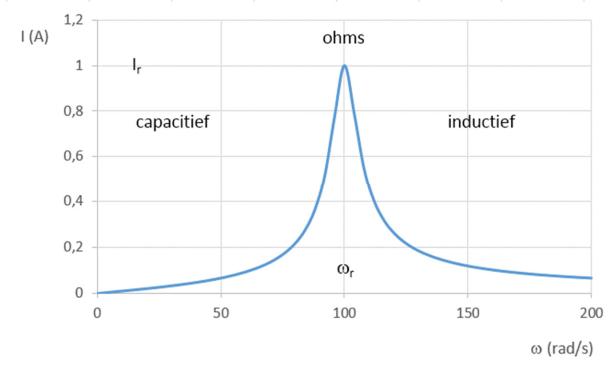
\includegraphics[width=0.7\textwidth]{assets/resonatie.png}
    \caption{Resonantie in een RLC-seriekring. Bij de resonantiefrequentie $f_0$ zijn de inductieve en capacitieve reactanties gelijk, waardoor de totale impedantie minimaal is en de stroom maximaal.}
    \label{fig:resonatie.png}
\end{figure}
\FloatBarrier

\subsubsection{Serie versus parallel: de stroom doet net het omgekeerde}

Dit is de valkuil die op het examen terugkomt. Serie- en parallelresonantie gebeuren allebei wanneer
$\text{Im}\{\underline{Z}\} = 0$, maar het gevolg is tegengesteld:

\begin{center}
    \begin{tabular}{@{}p{34mm}p{44mm}p{44mm}@{}}
        \toprule
                                  & \textbf{Serieresonantie}                          & \textbf{Parallelresonantie}                        \\
        \midrule
        Totale impedantie         & \textbf{minimaal} ($\underline{Z} = R$)           & \textbf{maximaal} ($\underline{Z} = R_p$)          \\[1mm]
        Bronstroom                & \textbf{maximaal}                                 & \textbf{minimaal}                                  \\[1mm]
        Bijnaam                   & spanningsopslingering over $L$ en $C$             & stroomopslingering \emph{binnen} de kring          \\[1mm]
        $\omega < \omega_0$       & capacitief                                        & inductief                                          \\[1mm]
        $\omega > \omega_0$       & inductief                                         & capacitief                                         \\
        \bottomrule
    \end{tabular}
\end{center}

Bij een parallelkring met een re\"ele spoel ($R$ in serie met $L$) is de bronstroom bij resonantie
niet nul, maar wel zo klein mogelijk:
\[\underline{I}_r = \frac{V R}{(\omega L)^2} = \frac{V R C}{L} = \frac{V}{R_p}\]
Met een \emph{ideale} spoel ($R = 0$) zou de bronstroom exact nul worden: de spoel en de condensator
wisselen dan onderling energie uit zonder dat de bron er iets aan hoeft bij te dragen.

\begin{figure}[htbp]
    \centering
    \begin{tikzpicture}[x=2.1cm, y=0.9cm, >=latex]
        % serie: stroom maximaal
        \begin{scope}
            \draw[->, gray] (0,0) -- (2.5,0) node[right, font=\scriptsize, black] {$f$};
            \draw[->, gray] (0,0) -- (0,2.6) node[above, font=\scriptsize, black] {$I$};
            \draw[ultra thick, schoolBlue, smooth, samples=80, domain=0.12:2.35]
                plot (\x, {2.2/sqrt(1+16*((\x/1.1)-(1.1/\x))^2)});
            \draw[dashed, gray!70] (1.1,0) -- (1.1,2.3);
            \node[font=\scriptsize, below] at (1.1,-0.06) {$f_0$};
            \node[font=\scriptsize\bfseries, anchor=north, align=center] at (1.25,-0.45) {seriekring:\\stroom \textbf{maximaal}};
        \end{scope}
        % parallel: stroom minimaal
        \begin{scope}[shift={(3.4,0)}]
            \draw[->, gray] (0,0) -- (2.5,0) node[right, font=\scriptsize, black] {$f$};
            \draw[->, gray] (0,0) -- (0,2.6) node[above, font=\scriptsize, black] {$I$};
            \draw[ultra thick, schoolRed, smooth, samples=80, domain=0.45:2.35]
                plot (\x, {0.35 + 2.0*abs((\x/1.1)-(1.1/\x))/2.6});
            \draw[dashed, gray!70] (1.1,0) -- (1.1,2.3);
            \node[font=\scriptsize, below] at (1.1,-0.06) {$f_0$};
            \node[font=\scriptsize, schoolRed, right] at (1.30,0.22) {$I_r = VRC/L$};
            \draw[schoolRed, thin] (1.28,0.26) -- (1.12,0.38);
            \node[font=\scriptsize\bfseries, anchor=north, align=center] at (1.25,-0.45) {parallelkring:\\stroom \textbf{minimaal}};
        \end{scope}
    \end{tikzpicture}
    \caption{De bronstroom in functie van de frequentie. Links een seriekring: bij $f_0$ valt de
        reactantie weg, blijft alleen $R$ over en piekt de stroom. Rechts een parallelkring: daar is
        de impedantie bij $f_0$ juist het \emph{grootst}, dus zakt de bronstroom naar een minimum.}
    \label{fig:resonantie-serie-parallel}
\end{figure}
\FloatBarrier


\section{Hoofdstuk 3: Elektrische netwerken}

De boodschap van dit hoofdstuk is eenvoudig: \textbf{alle netwerkanalyse die je vorig jaar bij
    Elektrische Netwerken leerde, werkt onveranderd op wisselstroom}. Serie en parallel, spannings- en
stroomdeling, knooppuntanalyse, Thévenin en Norton --- allemaal identiek.

Het enige verschil is dat je nu met \textbf{complexe} impedanties $\underline{Z}$ rekent in
plaats van met reële weerstanden $R$. Laat je daardoor niet afschrikken: de regels blijven dezelfde,
alleen je rekenmachine moet in complexe modus staan.

Wat wél nieuw is, zijn de \emph{werkwijzen} verderop in dit hoofdstuk: wanneer je achterwaarts
rekent met een correctiefactor, wanneer je knooppuntanalyse gebruikt, en hoe je een oefening aanpakt
waarin je alleen de \emph{groottes} van stromen kent.

\frm{Belastingen in serie}{Z_{totaal} = Z_1 + Z_2 + ... + Z_n}{Met $Z_{totaal}$ de totale impedantie in Ohm en $Z_1, Z_2, ..., Z_n$ de individuele impedanties in Ohm.}

\frm{Belastingen in parallel}{\frac{1}{Z_{totaal}} = \frac{1}{Z_1} + \frac{1}{Z_2} + ... + \frac{1}{Z_n}}{Met $Z_{totaal}$ de totale impedantie in Ohm en $Z_1, Z_2, ..., Z_n$ de individuele impedanties in Ohm.}

In parallel:
\[Z_{totaal} = \frac{1}{\frac{1}{Z_1} + \frac{1}{Z_2}} = \frac{Z_1 Z_2}{Z_1 + Z_2}\]

\frm{Brontransformatie (Thévenin $\leftrightarrow$ Norton)}{\underline{V}_{\text{th}} = \underline{I}_{\text{no}} \cdot \underline{Z}_{\text{th}} \qquad , \qquad \underline{Z}_{\text{th}} = \underline{Z}_{\text{no}}}
{Een reële spanningsbron ($\underline{V}_{\text{th}}$ in serie met $\underline{Z}_{\text{th}}$) is
    volledig equivalent aan een reële stroombron ($\underline{I}_{\text{no}}$ parallel aan $\underline{Z}_{\text{no}}$).
    Let op het pijlteken van de stroombron: de stroom wijst naar de positieve pool van de spanningsbron.}

Zorg dat je niet verward geraakt omdat capaciteiten en inductanties imaginaire impedanties zijn.
Je gebruikt gewoon dezelfde regels als bij DC netwerken.


\begin{examenbox}
    Zorg dat je de slides van dit hoofdstuk goed bekijkt.
    Thevenin en Norton komen hier terug aan bod.
    Als je vorig jaar elektrische netwerken goed begreep zou dit ook moeten lukken.
\end{examenbox}

\subsection{Spanningsdeling en stroomdeling}

Deze twee gebruik je in bijna elke 1-fase oefening, dus ze moeten er vlot in zitten.

\frm{Spanningsdeling (serie)}{\underline{V}_1 = \underline{V} \cdot \frac{\underline{Z}_1}{\underline{Z}_1 + \underline{Z}_2}}
{Met $\underline{V}_1$ de spanning over $\underline{Z}_1$ in V, $\underline{V}$ de totale spanning
    over beide impedanties in V, en $\underline{Z}_1,\underline{Z}_2$ de twee serie-impedanties in $\Omega$.}

\frm{Stroomdeling (parallel)}{\underline{I}_1 = \underline{I} \cdot \frac{\underline{Z}_2}{\underline{Z}_1 + \underline{Z}_2}}
{Met $\underline{I}_1$ de stroom door $\underline{Z}_1$ in A, $\underline{I}$ de totale stroom die
    zich splitst in A, en $\underline{Z}_1,\underline{Z}_2$ de twee parallelle impedanties in $\Omega$.}

\begin{waarschuwing}[Let op welke impedantie in de teller staat]
    Bij \textbf{spanningsdeling} staat in de teller de \textbf{eigen} impedantie.
    Bij \textbf{stroomdeling} staat in de teller de impedantie van de \textbf{andere} tak.

    Dat is logisch: door de tak met de \emph{kleinste} impedantie loopt de \emph{grootste} stroom,
    dus de breuk moet klein worden als je eigen impedantie groot is.
\end{waarschuwing}

\begin{oefening}[Voorbeeld uit slides: Parallelschakeling van twee takken (RL en RC)]
    \textbf{Opgave:}
    Een bron met spanning $\underline{V} = 200\angle 0^\circ\text{ V}$ ($f = 50\text{ Hz}$, $\omega = 314\text{ rad/s}$) voedt twee parallelle takken:
    \begin{itemize}
        \item \textbf{Tak 1 (inductief):} weerstand $R_1 = 50\,\Omega$ in serie met spoel $L = 0{,}318\text{ H}$.
        \item \textbf{Tak 2 (capacitief):} weerstand $R_2 = 80\,\Omega$ in serie met condensator $C = 159\,\mu\text{F}$.
    \end{itemize}
    Bereken de takimpedanties, takstromen, deelspanningen, totale stroom $\underline{I}_{\text{tot}}$ en totale impedantie $\underline{Z}_{\text{tot}}$.

    \begin{center}
        \begin{circuitikz}[scale=0.85, transform shape]
            \draw (0,0) to[sV={$200\angle 0^\circ$~V}, i<^=$\underline{I}_{\text{tot}}$] (0,4.0);
            \draw (0,4.0) node[circ]{} -- (5.6,4.0);
            \draw (2.8,4.0) node[circ]{} to[R, l_={$R_1 = 50\,\Omega$}, i>^=$\underline{I}_1$] (2.8,2.2)
                  to[L, l_={$L = 0{,}318$~H}] (2.8,0);
            \draw (5.6,4.0) to[R, l={$R_2 = 80\,\Omega$}, i>^=$\underline{I}_2$] (5.6,2.2)
                  to[C, l={$C = 159\,\mu$F}] (5.6,0) node[circ]{};
            \draw (0,0) -- (5.6,0);
            \draw (0,0) node[ground]{};
        \end{circuitikz}
    \end{center}

    \textbf{Oplossing:}
    \begin{enumerate}
        \item \textbf{Takimpedanties:}
              \begin{itemize}
                  \item Tak 1: $X_L = \omega L = 314 \cdot 0{,}318 = 100\,\Omega \implies \underline{Z}_1 = 50 + j100\,\Omega = 111{,}8\angle 63{,}4^\circ\,\Omega$.
                  \item Tak 2: $X_C = -\frac{1}{\omega C} = -\frac{1}{314 \cdot 159 \cdot 10^{-6}} = -20\,\Omega \implies \underline{Z}_2 = 80 - j20\,\Omega = 82{,}5\angle -14{,}0^\circ\,\Omega$.
              \end{itemize}
        \item \textbf{Takstromen (wet van Ohm):}
              \[\underline{I}_1 = \frac{\underline{V}}{\underline{Z}_1} = \frac{200\angle 0^\circ}{111{,}8\angle 63{,}4^\circ} = 1{,}79\angle -63{,}4^\circ\text{ A} = 0{,}80 - j1{,}60\text{ A}\]
              \[\underline{I}_2 = \frac{\underline{V}}{\underline{Z}_2} = \frac{200\angle 0^\circ}{82{,}5\angle -14{,}0^\circ} = 2{,}42\angle +14{,}0^\circ\text{ A} = 2{,}35 + j0{,}59\text{ A}\]
        \item \textbf{Deelspanningen:}
              \begin{itemize}
                  \item Tak 1: $V_{R1} = 50 \cdot 1{,}79 = 89{,}5\text{ V}$ en $V_L = 100 \cdot 1{,}79 = 179\text{ V}$ (merk op: $\sqrt{89{,}5^2 + 179^2} = 200\text{ V}$).
                  \item Tak 2: $V_{R2} = 80 \cdot 2{,}42 = 193{,}6\text{ V}$ en $V_C = 20 \cdot 2{,}42 = 48{,}4\text{ V}$ (merk op: $\sqrt{193{,}6^2 + 48{,}4^2} = 200\text{ V}$).
              \end{itemize}
        \item \textbf{Totale stroom en vervangingsimpedantie:}
              \[\underline{I}_{\text{tot}} = \underline{I}_1 + \underline{I}_2 = (0{,}80 + 2{,}35) + j(-1{,}60 + 0{,}59) = 3{,}15 - j1{,}01\text{ A} = \mathbf{3{,}31\angle -17{,}8^\circ\text{ A}}\]
              \[\underline{Z}_{\text{tot}} = \frac{\underline{V}}{\underline{I}_{\text{tot}}} = \frac{200\angle 0^\circ}{3{,}31\angle -17{,}8^\circ} = \mathbf{60{,}4\angle +17{,}8^\circ\,\Omega} = 57{,}5 + j18{,}5\,\Omega\]
    \end{enumerate}
\end{oefening}

\begin{oefening}[Sadiku Probleem 10.7: Brontransformatie en Stroomdeling]
    \textbf{Opgave:}
    Een spanningsbron $\underline{V}_s = 60\angle 53{,}1^\circ\text{ V}$ staat in serie met impedanties $(4 - j3)\,\Omega$ en $(2 + j)\,\Omega$.
    Hierachter staat een parallelle tak met impedantie $j5\,\Omega$, gevolgd door een belasting $\underline{Z}_L = 1 - j2\,\Omega$.
    Bepaal de stroom $\underline{I}_o$ door de belasting via opeenvolgende brontransformatie.

    \begin{center}
        \begin{circuitikz}[scale=0.85, transform shape]
            \draw (0,0) to[sV={$60\angle 53{,}1^\circ$~V}] (0,3.4);
            \draw (0,3.4) to[generic={$4-j3\,\Omega$}] (2.8,3.4)
                  to[generic={$2+j\,\Omega$}] (5.6,3.4) node[circ]{};
            \draw (5.6,3.4) to[generic={$j5\,\Omega$}] (5.6,0);
            \draw (5.6,3.4) -- (8.4,3.4) to[generic={$\underline{Z}_L = 1-j2\,\Omega$}, i>^=$\underline{I}_o$] (8.4,0) node[circ]{};
            \draw (0,0) -- (8.4,0);
            \draw (0,0) node[ground]{};
        \end{circuitikz}
    \end{center}

    \textbf{Oplossing:}
    \begin{enumerate}
        \item \textbf{Serie-impedantie bij de bron:}
              $\underline{Z}_1 = (4 - j3) + (2 + j) = 6 - j2\,\Omega = 6{,}325\angle -18{,}43^\circ\,\Omega$.
        \item \textbf{Omzetting naar Norton-stroombron:}
              \[\underline{I}_{\text{no}} = \frac{\underline{V}_s}{\underline{Z}_1} = \frac{60\angle 53{,}1^\circ}{6{,}325\angle -18{,}43^\circ} = 9{,}487\angle 71{,}53^\circ\text{ A}\]
        \item \textbf{Parallelschakeling $\underline{Z}_1 \parallel j5\,\Omega$:}
              \[\underline{Z}_p = \frac{(6 - j2) \cdot j5}{(6 - j2) + j5} = \frac{10 + j30}{6 + j3} = \frac{31{,}62\angle 71{,}57^\circ}{6{,}708\angle 26{,}57^\circ} = 4{,}714\angle 45{,}0^\circ\,\Omega = 3{,}333 + j3{,}333\,\Omega\]
        \item \textbf{Stroomdeling naar $\underline{Z}_L = 1 - j2\,\Omega$:}
              \[\underline{I}_o = \underline{I}_{\text{no}} \cdot \frac{\underline{Z}_p}{\underline{Z}_p + \underline{Z}_L} = 9{,}487\angle 71{,}53^\circ \cdot \frac{3{,}333 + j3{,}333}{(3{,}333 + 1) + j(3{,}333 - 2)} = 9{,}487\angle 71{,}53^\circ \cdot \frac{4{,}714\angle 45{,}0^\circ}{4{,}333 + j1{,}333}\]
              Met $4{,}333 + j1{,}333 = 4{,}533\angle 17{,}10^\circ\,\Omega$ vinden we:
              \[\underline{I}_o = \frac{9{,}487 \cdot 4{,}714}{4{,}533} \angle (71{,}53^\circ + 45{,}0^\circ - 17{,}10^\circ) = \mathbf{9{,}87\angle 99{,}4^\circ\text{ A}}\]
    \end{enumerate}
\end{oefening}

\subsection{Een net oplossen: welke methode kies je?}

Er zijn verschillende werkwijzen, en de keuze hangt af van het aantal bronnen en de netwerktopologie.

\subsubsection{Methode 1: achterwaarts rekenen met een correctiefactor}

Gebruik dit bij \textbf{één bron} en een net dat een ketting is van serie- en
parallelverbindingen. Vooruit rekenen zou een stelsel geven; achteruit rekenen is één rechte lijn.

\begin{theorie}[Werkwijze]
    \begin{enumerate}
        \item \textbf{Kies} \emph{achteraan} in het net zelf een waarde, bijvoorbeeld
              $\underline{V}_b = 200\angle 0^\circ$~V over de laatste tak. Die neem je meteen als
              referentie (hoek $0^\circ$).
        \item Reken van achter naar voor: takstromen met de wet van Ohm, samenvoegen met KCL,
              spanningsvallen erbij optellen tot je aan de bron komt. Alles wat je zo vindt noem je
              \emph{berekend}.
        \item Je komt uit op een bronspanning $\underline{V}_{\text{berekend}}$, die
              natuurlijk niet gelijk is aan de werkelijke bronspanning.
        \item Bereken de \textbf{correctiefactor}
              \[\underline{k} = \frac{\underline{V}_{\text{werkelijk}}}{\underline{V}_{\text{berekend}}}\]
        \item Vermenigvuldig \textbf{alle} tussenresultaten met $\underline{k}$.
    \end{enumerate}
\end{theorie}

\begin{figure}[htbp]
    \centering
    \begin{circuitikz}[scale=0.88, transform shape]
        \draw (0,0) node[circ]{} node[below]{$A$}
              to[sV={$230$~V / 50~Hz}] (0,3.6) node[circ]{} node[above]{$C$};
        \draw (0,3.6) to[R, l={$R_1 = 4\,\Omega$}, i>^=$\underline{I}_1$] (4.0,3.6)
              node[circ]{} node[above]{$B$};
        \draw (4.0,3.6) -- (6.6,3.6);
        \draw (4.0,3.6) to[L, l_={$X_L = 100\,\Omega$}, i>^=$\underline{I}_2$] (4.0,0);
        \draw (6.6,3.6) to[R, l_={$R_2 = 50\,\Omega$}, i>^=$\underline{I}_3$] (6.6,0) node[circ]{};
        \draw (0,0) -- (6.6,0);
        \draw[<->, thick, schoolBlue] (8.4,3.6) -- (8.4,0);
        \node[font=\footnotesize, schoolBlue, right, align=left] at (8.55,1.8) {$\underline{V}_b$\\\scriptsize (gezocht)};
        \draw[dashed, gray!70] (6.6,3.6) -- (8.4,3.6);
        \draw[dashed, gray!70] (6.6,0) -- (8.4,0);
        \draw (0,0) node[ground]{};
    \end{circuitikz}
    \caption{Het net uit de cursus. Je zoekt $\underline{V}_b$ over de verbruikers, maar de bron
        staat aan de \emph{andere} kant van de lijnweerstand $R_1$. Vooruit rekenen zou een stelsel
        geven; achterwaarts rekenen is \'e\'en rechte lijn --- vandaar de omweg via een gekozen waarde
        en een correctiefactor.}
    \label{fig:methode1-net}
\end{figure}
\FloatBarrier

\begin{oefening}[Voorbeeld uit slides: achterwaarts rekenen met een correctiefactor]
    \textbf{Opgave:}
    Een netwerk wordt gevoed met $V_{\text{net}} = 230\text{ V} / 50\text{ Hz}$.
    Een leidingweerstand $R_1 = 4\,\Omega$ staat in serie met de parallelcombinatie van een verbruiker $R_2 = 50\,\Omega$ en een spoel met $X_L = 100\,\Omega$.
    Zoek de werkelijke spanning $\underline{V}_2$ over de verbruikers en de bronstroom $\underline{I}_{\text{bron}}$.

    \textbf{Oplossing:} (zie het schema in figuur~\ref{fig:methode1-net})
    \begin{enumerate}
        \item \textbf{Kies zelf een waarde achteraan:} $\underline{V}_b = 200\angle 0^\circ$~V, meteen als referentie.
        \item \textbf{Takstromen achteraan:}
              \[\underline{I}_3 = \frac{200\angle 0^\circ}{50} = 4\text{ A} \qquad,\qquad \underline{I}_2 = \frac{200\angle 0^\circ}{j100} = -j2\text{ A}\]
              $\underline{I}_3$ ligt in fase met $\underline{V}_b$ (weerstand), $\underline{I}_2$ ijlt $90^\circ$ na (spoel).
        \item \textbf{Totale stroom met KCL:} $\underline{I}_1 = 4 - j2\text{ A} = 4{,}472\angle -26{,}57^\circ\text{ A}$.
        \item \textbf{Spanningsval over de lijn en de bijhorende bronspanning:}
              \[\underline{V}_{R1} = R_1 \cdot \underline{I}_1 = 4 \cdot (4 - j2) = 16 - j8\text{ V}\]
              \[\underline{V}_{\text{berekend}} = \underline{V}_b + \underline{V}_{R1} = 200 + (16 - j8) = 216 - j8\text{ V} = 216{,}15\angle -2{,}12^\circ\text{ V}\]
        \item \textbf{Correctiefactor $\underline{k}$:}
              \[\underline{k} = \frac{\underline{V}_{\text{werkelijk}}}{\underline{V}_{\text{berekend}}} = \frac{230\angle 0^\circ}{216{,}15\angle -2{,}12^\circ} = 1{,}0641\angle +2{,}12^\circ\]
        \item \textbf{Alles vermenigvuldigen met $\underline{k}$:}
              \[\underline{V}_b = \underline{k} \cdot 200\angle 0^\circ = \mathbf{212{,}8\angle 2{,}12^\circ\text{ V}}\]
              \[\underline{I}_1 = \underline{k} \cdot 4{,}472\angle -26{,}57^\circ = \mathbf{4{,}76\angle -24{,}45^\circ\text{ A}}\]
    \end{enumerate}
    De lijn ``kost'' dus ongeveer $17$~V, ruim $7\%$ spanningsval --- in de praktijk te veel, want de
    norm laat meestal $5\%$ toe.
\end{oefening}

\begin{examenbox}[EXAMENVRAAG:]
    \textit{Waarom hoef je bij deze methode de hoeken niet apart te corrigeren?}

    Omdat de keten \textbf{lineair} is. Elk resultaat heeft de vorm
    $\underline{X} = \underline{H}\cdot\underline{V}_b$, waarbij $\underline{H}$ alleen van de
    impedanties afhangt. Vervang je $\underline{V}_b$ door $\underline{k}\,\underline{V}_b$, dan wordt
    élke spanning en élke stroom met dezelfde factor $\underline{k}$ vermenigvuldigd.

    Is $\underline{k}$ reëel, dan verandert er niets aan de hoeken: het hele fasordiagramma wordt
    gewoon groter of kleiner. Is $\underline{k}$ complex, dan draait het hele diagramma over
    $\arg(\underline{k})$, maar de
    \textbf{onderlinge} hoeken blijven gelijk. En die onderlinge hoeken zijn precies wat de
    arbeidsfactoren en de vermogens bepalen. Je hoeft dus nooit hoek per hoek te corrigeren.
\end{examenbox}

Kijk wel eerst \emph{waar} de gegeven waarde staat. Staat de gegeven spanning binnenin het
net (bijvoorbeeld ``de spanning over de spoel is 200~V'' of een voltmeteraflezing), dan is dat al je
referentie: reken gewoon van daaruit naar voor, zonder correctiestap.

\subsubsection{Methode 2: knooppuntanalyse (KCL)}

Gebruik dit zodra er \textbf{meerdere bronnen} zijn, of wanneer het net geen zuivere
serie-parallelstructuur heeft.

\begin{theorie}[Werkwijze]
    \begin{enumerate}
        \item Zet alles om naar het frequentiedomein ($\underline{Z}_L = j\omega L$,
              $\underline{Z}_C = -j/(\omega C)$).
        \item Kies één knoop als \textbf{aarde}. Kies bij voorkeur de knoop waar de meeste takken
              samenkomen, of de knoop waarop een bron rechtstreeks aansluit --- dan ligt die
              knoopspanning meteen vast.
        \item Tel de onbekende knoopspanningen: dat is het aantal vergelijkingen dat je nodig hebt.
        \item Schrijf per onbekende knoop de KCL op: de som van alle \emph{uitgaande} stromen is nul.
              Elke tak levert een term $(\underline{V}_{\text{knoop}} - \underline{V}_{\text{buur}})/\underline{Z}$.
              Een stroombron die \emph{in} de knoop duwt, komt er met een minteken bij.
        \item Los het stelsel op met je rekenmachine in complexe modus.
        \item Bereken daarna de gevraagde takstromen met de wet van Ohm.
    \end{enumerate}
\end{theorie}

\begin{figure}[htbp]
    \centering
    \begin{circuitikz}[scale=0.88, transform shape]
        \draw (0,0) to[sV={$\underline{V}_{s1}$}] (0,3.6);
        \draw (0,3.6) to[generic={$\underline{Z}_1$}] (3.2,3.6) node[circ]{};
        \node[font=\small, above, schoolBlue] at (3.2,3.8) {knoop $\underline{V}_A$};
        \draw (3.2,3.6) to[generic={$\underline{Z}_3$}] (6.4,3.6) node[circ]{};
        \node[font=\small, above, schoolBlue] at (6.4,3.8) {knoop $\underline{V}_B$};
        \draw (3.2,3.6) to[generic={$\underline{Z}_2$}] (3.2,0);
        \draw (6.4,3.6) to[generic={$\underline{Z}_4$}] (6.4,0);
        \draw (6.4,3.6) -- (9.0,3.6) to[I={$\underline{I}_{s2}$}] (9.0,0) node[circ]{};
        \draw (0,0) -- (9.0,0);
        \node[font=\small, below, schoolRed] at (4.5,-0.15) {referentieknoop (aarde), $\underline{V} = 0$};
        \draw (0,0) node[ground]{};
    \end{circuitikz}
    \caption{Waar knooppuntanalyse voor dient. Dit net is g\'e\'en ketting van serie- en
        parallelverbindingen (er zijn twee bronnen), dus achterwaarts rekenen werkt niet. Kies de
        onderste rail als referentie; dan blijven er twee onbekende knoopspanningen
        $\underline{V}_A$ en $\underline{V}_B$ over, en dus twee KCL-vergelijkingen. In knoop $A$:
        $\frac{\underline{V}_A - \underline{V}_{s1}}{\underline{Z}_1} + \frac{\underline{V}_A}{\underline{Z}_2}
        + \frac{\underline{V}_A - \underline{V}_B}{\underline{Z}_3} = 0$.}
    \label{fig:kcl-opzet}
\end{figure}
\FloatBarrier

\begin{examenbox}
    \textbf{Controleer altijd met KCL} in elke knoop nadat je de takstromen hebt. Het kost je een
    halve minuut en het vindt bijna elke rekenfout. Doe daarnaast ook de vermogensbalans
    $P_{\text{bron}} = \sum I^2R$.
\end{examenbox}

\subsubsection{Methode 3: Superpositie bij bronnen met verschillende frequenties}

Wanneer een lineaire keten meerdere onafhankelijke bronnen bevat met \textbf{verschillende frequenties}
($\omega_1 \neq \omega_2$), is de fasormethode niet direct toepasbaar op het hele circuit omdat fasors
slechts geldig zijn voor één specifieke frequentie.

\begin{theorie}[Werkwijze bij superpositie]
    \begin{enumerate}
        \item Schakel telkens \textbf{één bron tegelijk} in (andere spanningsbronnen kortsluiten, stroombronnen openen).
        \item Bepaal voor elke afzonderlijke bron de respons in het fasordomein bij de bijhorende pulsatie $\omega_i$.
        \item Zet elk fasor-deelresultaat om naar een \textbf{tijdsfunctie} (cosinus/sinus).
        \item Tel alle deelresultaten pas op in het \textbf{tijdsdomein}:
              \[v_{\text{totaal}}(t) = v_{(1)}(t) + v_{(2)}(t) + \dots + v_{(n)}(t)\]
    \end{enumerate}
\end{theorie}

\begin{oefening}[Voorbeeld uit slides: Superpositie met DC en meerdere AC-frequenties]
    \textbf{Opgave:}
    Bepaal de spanning $v_o(t)$ in een keten met:
    \begin{itemize}
        \item DC-spanningsbron $V_1 = 5\text{ V}$ ($\omega_1 = 0\text{ rad/s}$)
        \item AC-spanningsbron $v_2(t) = 10\cos(2t)\text{ V}$ ($\omega_2 = 2\text{ rad/s}$)
        \item AC-stroombron $i_3(t) = 2\sin(5t)\text{ A}$ ($\omega_3 = 5\text{ rad/s}$)
    \end{itemize}
    geschakeld in het net hieronder, met $L = 2$~H, $C = 0{,}1$~F en twee weerstanden van
    $1\,\Omega$ en $4\,\Omega$. De gezochte spanning $v_o$ staat over de $1\,\Omega$.

    \begin{center}
        \begin{circuitikz}[scale=0.82, transform shape]
            \draw (0,0) to[sV={$10\cos 2t$~V}] (0,3.0);
            \draw (0,3.0) to[L, l={$2$~H}] (2.6,3.0) node[circ]{};
            \draw (2.6,3.0) to[I={$2\sin 5t$~A}] (2.6,0) node[circ]{};
            \draw (2.6,3.0) to[R, l={$1\,\Omega$}, v^>={$v_o$}] (5.8,3.0) node[circ]{};
            \draw (5.8,3.0) to[C, l_={$0{,}1$~F}] (5.8,0) node[circ]{};
            \draw (5.8,3.0) to[R, l={$4\,\Omega$}] (8.8,3.0);
            \draw (8.8,3.0) to[battery1, l_={$5$~V}] (8.8,0);
            \draw (0,0) -- (8.8,0);
            \draw (0,0) node[ground]{};
        \end{circuitikz}
    \end{center}

    \textbf{Oplossing:}
    \begin{enumerate}
        \item \textbf{Deelrespons DC ($\omega_1 = 0$):}
              Op DC is de condensator een open keten ($Z_C = \infty$) en de spoel een kortsluiting ($Z_L = 0$).
              De $5$~V staat dan over $4\,\Omega + 1\,\Omega$ in serie, dus $I = 1$~A en
              $V_{o,1} = 1\,\Omega \cdot 1\text{ A} = 1\text{ V}$.
        \item \textbf{Deelrespons $v_2(t)$ ($\omega_2 = 2\text{ rad/s}$):}
              $\underline{V}_2 = 10\angle 0^\circ\text{ V}$, $\underline{Z}_L = j\omega L = j(2)(2) = j4\,\Omega$, $\underline{Z}_C = \frac{1}{j(2)(0{,}1)} = -j5\,\Omega$.
              Uit spanningsdeling: $\underline{V}_{o,2} = 2{,}498\angle -30{,}8^\circ\text{ V} \implies v_{o,2}(t) = 2{,}498\cos(2t - 30{,}8^\circ)\text{ V}$.
        \item \textbf{Deelrespons $i_3(t)$ ($\omega_3 = 5\text{ rad/s}$):}
              $i_3(t) = 2\cos(5t - 90^\circ)\text{ A} \implies \underline{I}_3 = 2\angle -90^\circ\text{ A}$.
              $\underline{Z}_L = j\omega L = j(5)(2) = j10\,\Omega$, $\underline{Z}_C = \frac{1}{j(5)(0{,}1)} = -j2\,\Omega$.
              Uit stroomdeling: $\underline{V}_{o,3} = 2{,}33\angle -80{,}0^\circ\text{ V} \implies v_{o,3}(t) = 2{,}33\cos(5t - 80{,}0^\circ)\text{ V} = 2{,}33\sin(5t + 10^\circ)\text{ V}$.
        \item \textbf{Totale tijdsoplossing:}
              \[\mathbf{v_o(t) = 1 + 2{,}498\cos(2t - 30{,}8^\circ) + 2{,}33\sin(5t + 10^\circ)\text{ V}}\]
    \end{enumerate}
\end{oefening}

\subsection{Thévenin equivalent en Maximale vermogenoverdracht}

\begin{oefening}[Sadiku Probleem 10.8: Thévenin equivalent in AC]
    \textbf{Opgave:}
    Bepaal het Thévenin-equivalent $(\underline{V}_{\text{th}}, \underline{Z}_{\text{th}})$ gezien vanaf klemmen $a-b$ van een netwerk met een spanningsbron $\underline{V}_s = 120\angle 75^\circ\text{ V}$ over een tak $(6 + j2)\,\Omega$ parallel met $-j4\,\Omega$, in serie met $10\,\Omega$.

    \begin{center}
        \begin{circuitikz}[scale=0.85, transform shape]
            \draw (0,0) to[sV={$120\angle 75^\circ$~V}] (0,3.4);
            \draw (0,3.4) to[generic={$6+j2\,\Omega$}] (3.4,3.4) node[circ]{};
            \draw (3.4,3.4) to[C, l_={$-j4\,\Omega$}] (3.4,0);
            \draw (3.4,3.4) to[R, l={$10\,\Omega$}] (6.8,3.4);
            \draw (6.8,3.4) -- (7.6,3.4) node[circ]{} node[above]{$a$};
            \draw (3.4,0) -- (7.6,0) node[circ]{} node[below]{$b$};
            \draw (0,0) -- (3.4,0);
            \node[font=\scriptsize, schoolRed, align=center, right] at (7.8,1.7) {open klemmen:\\hier loopt geen stroom,\\dus geen val over $10\,\Omega$};
            \draw (0,0) node[ground]{};
        \end{circuitikz}
    \end{center}

    \textbf{Oplossing:}
    \begin{enumerate}
        \item \textbf{Thévenin-impedantie $\underline{Z}_{\text{th}}$ (deactiveer de spanningsbron):}
              De bron wordt kortgesloten. De tak $(6 + j2)\,\Omega$ staat parallel met $-j4\,\Omega$:
              \[\underline{Z}_p = (6 + j2) \parallel (-j4) = \frac{(6 + j2)(-j4)}{6 + j2 - j4} = \frac{8 - j24}{6 - j2} = 2{,}4 - j3{,}2\,\Omega\]
              Hier staat de serieweerstand $10\,\Omega$ mee in serie:
              \[\underline{Z}_{\text{th}} = 10 + \underline{Z}_p = \mathbf{12{,}4 - j3{,}2}\ \Omega\]
        \item \textbf{Thévenin-openklemspanning $\underline{V}_{\text{th}}$:}
              Omdat er aan klemmen $a-b$ geen stroom loopt door de serieweerstand van $10\,\Omega$, is $\underline{V}_{\text{th}}$ gelijk aan de spanning over de parallelle condensator $-j4\,\Omega$ via spanningsdeling:
              \[\underline{V}_{\text{th}} = \underline{V}_s \cdot \frac{-j4}{(6 + j2) - j4} = 120\angle 75^\circ \cdot \frac{4\angle -90^\circ}{6{,}325\angle -18{,}43^\circ} = \mathbf{75{,}89\angle 3{,}43^\circ\text{ V}}\]
    \end{enumerate}
\end{oefening}

\frm{Maximale vermogenoverdracht in AC}{\underline{Z}_L = \underline{Z}_{\text{th}}^* = R_{\text{th}} - jX_{\text{th}} \qquad \Longrightarrow \qquad P_{\text{max}} = \frac{|\underline{V}_{\text{th}}|^2}{4 R_{\text{th}}}}
{Voor maximale overdracht van \textbf{actief vermogen} aan een wisselstroombelasting $\underline{Z}_L = R_L + jX_L$ moet de belastingsimpedantie de \textbf{complex geconjugeerde} zijn van de Thévenin-impedantie $\underline{Z}_{\text{th}} = R_{\text{th}} + jX_{\text{th}}$.
    De reactanties heffen elkaar dan op ($X_L = -X_{\text{th}}$), waardoor totale resonantie optreedt.
    \newline
    \textbf{Speciaal geval (zuiver ohmse belasting $R_L$):} kan je geen reactantie kiezen, dan is
$X_L = 0$ en treedt het maximum op wanneer
\[R_L = |\underline{Z}_{\text{th}}| = \sqrt{R_{\text{th}}^2 + X_{\text{th}}^2}
    \qquad\Longrightarrow\qquad
    P_{L,\max} = \frac{V_{\text{th}}^2}{2\left(R_{\text{th}} + |\underline{Z}_{\text{th}}|\right)}\]
Dat maximum ligt altijd \emph{lager} dan wat je met een aangepaste complexe belasting haalt: je kan
de reactantie van de bron nu immers niet wegcompenseren.}

\subsubsection{Waar die twee voorwaarden vandaan komen}

Je hoeft dit niet als bewijs te kunnen reproduceren, maar als je de afleiding \'e\'en keer volgt,
hoef je $\underline{Z}_L = \underline{Z}_{\text{th}}^{*}$ nooit meer uit het hoofd te leren --- je
ziet dan gewoon waarom het zo moet zijn.

\stapreden{Vervang alles door het Th\'evenin-equivalent en zet er een belasting $\underline{Z}_L = R_L + jX_L$ op. De stroom volgt uit de wet van Ohm:}
\[\underline{I}_L = \frac{\underline{V}_{\text{th}}}{\underline{Z}_{\text{th}} + \underline{Z}_L}
    \qquad\Longrightarrow\qquad
    I_L = \frac{V_{\text{th}}}{\sqrt{(R_{\text{th}}+R_L)^2 + (X_{\text{th}}+X_L)^2}}\]

\stapreden{Alleen de weerstand van de last zet vermogen om, dus:}
\[P_L = R_L\,I_L^2 = \frac{V_{\text{th}}^2\,R_L}{(R_{\text{th}}+R_L)^2 + (X_{\text{th}}+X_L)^2}\]

\stapreden{\textbf{Eerst $X_L$.} Die staat alleen in de noemer, en wel in een kwadraat. De breuk is dus het grootst wanneer dat kwadraat het kleinst is, en dat is nul:}
\[\frac{\partial P_L}{\partial X_L}
    = \frac{-2V_{\text{th}}^2 R_L (X_{\text{th}}+X_L)}{\left[(R_{\text{th}}+R_L)^2 + (X_{\text{th}}+X_L)^2\right]^2} = 0
    \qquad\Longrightarrow\qquad \boxed{X_L = -X_{\text{th}}}\]

Fysisch: de twee reactanties heffen elkaar op, de keten komt in resonantie en de stroom loopt weer
in fase met de spanning. Elke restreactantie zou een stuk van de spanning ``vasthouden'' zonder er
vermogen mee te leveren.

\stapreden{\textbf{Dan $R_L$}, met $X_{\text{th}}+X_L$ nu al nul:}
\[P_L = \frac{V_{\text{th}}^2\,R_L}{(R_{\text{th}}+R_L)^2}
    \qquad\Longrightarrow\qquad
    \frac{\partial P_L}{\partial R_L}
    = V_{\text{th}}^2\,\frac{(R_{\text{th}}+R_L)^2 - 2R_L(R_{\text{th}}+R_L)}{(R_{\text{th}}+R_L)^4} = 0\]

\stapreden{De teller nul stellen en delen door $(R_{\text{th}}+R_L)$:}
\[(R_{\text{th}}+R_L) - 2R_L = 0 \qquad\Longrightarrow\qquad \boxed{R_L = R_{\text{th}}}\]

\stapreden{Samen geven die twee precies de complex toegevoegde, en het maximum zelf volgt door in te vullen:}
\[\underline{Z}_L = R_{\text{th}} - jX_{\text{th}} = \underline{Z}_{\text{th}}^{*}
    \qquad\qquad
    P_{L,\max} = \frac{V_{\text{th}}^2 R_{\text{th}}}{(2R_{\text{th}})^2} = \frac{V_{\text{th}}^2}{4R_{\text{th}}}\]

\begin{waarschuwing}[Dit is geen rendement van 100\,\%]
    Bij aanpassing staat er evenveel weerstand in de bron als in de last, dus de bron verstookt
    \emph{evenveel} vermogen als ze afgeeft: het rendement is $50\%$. Je maximaliseert hier het
    \textbf{afgegeven} vermogen, niet de effici\"entie. In een energienet wil je precies het
    omgekeerde ($R_{\text{th}} \ll R_L$); aanpassing gebruik je bij signalen en antennes, waar het
    om het vermogen zelf gaat en niet om de energiefactuur.
\end{waarschuwing}

\subsection{Werken met enkel de grootte van stromen}

Soms geeft het examen je alleen \textbf{ampèremeteraflezingen}: drie stroomgrootten zonder
hoeken. Dat lijkt te weinig informatie, maar dat is het niet.

Vormen die drie stromen samen een KCL-knoop ($\underline{I}_1 = \underline{I}_2 + \underline{I}_3$),
dan vormen hun fasoren een \textbf{gesloten driehoek}. Met de cosinusregel haal je de
ontbrekende hoeken eruit.

\begin{theorie}[Werkwijze]
    \begin{enumerate}
        \item Kies één van de drie stromen als referentie, bijvoorbeeld
              $\underline{I}_1 = |I_1|\angle 0^\circ$.
        \item Pas de cosinusregel toe. De hoek $\theta$ \emph{tussen} $\underline{I}_1$ en
              $\underline{I}_2$ staat in de driehoek tegenover de zijde $|I_3|$:
              \[\cos\theta = \frac{|I_1|^2 + |I_2|^2 - |I_3|^2}{2|I_1||I_2|}\]
        \item Doe hetzelfde voor de tweede hoek, of gebruik dat de drie hoeken samen $180^\circ$ zijn.
        \item Ken je fysisch welke stroom voor- en welke naijlt, gebruik dat om de \emph{tekens}
              van de hoeken te bepalen.
        \item \textbf{Controleer} door de twee fasoren op te tellen: je moet de derde terugkrijgen.
    \end{enumerate}
\end{theorie}

\textbf{Hoe weet je welk teken?} Een condensatortak laat de stroom \textbf{voorijlen} (hoek
positief t.o.v.\ de spanning), een spoeltak laat hem \textbf{naijlen}. Staan beide takken over
dezelfde spanning, dan liggen hun stromen aan weerszijden van die spanning.

\subsection{Een fasordiagramma tekenen}

Bijna elke oefening vraagt dit, en er staan punten op. Twee regels:

\begin{itemize}
    \item \textbf{Spanningen teken je kop-staart.} Begin in een knoop, teken de spanningsval over
          de eerste tak, zet de staart van de volgende pijl aan de kop van de vorige, enzovoort.
          De pijl van begin- tot eindpunt is dan de totale spanning. Zo vallen de knooppunten samen
          met de hoekpunten van je diagramma, en die kan je benoemen --- dat wordt vaak expliciet
          gevraagd.
    \item \textbf{Stromen teken je allemaal vanuit één punt}, als een waaier.
\end{itemize}

Gebruik twee verschillende schalen, één voor spanningen en één voor stromen (bijvoorbeeld
$1:40$ voor V en $1:2$ voor A), en \textbf{schrijf ze bij het diagramma}. Zonder schaal is een
diagramma niet controleerbaar en verlies je punten. Neem je geodriehoek en passer mee: het moet op
schaal zijn, niet uit de losse hand.

\begin{oefening}[Voorbeeld uit slides: het fasordiagramma van het net van methode 1]
    \textbf{Opgave:} teken het fasordiagramma van alle spanningen en stromen van het net uit
    figuur~\ref{fig:methode1-net}, met de knooppunten $A$, $B$ en $C$ erbij.

    \textbf{Gegeven uit de berekening:}
    \[\underline{V}_b = 200\angle 0^\circ\ \text{V} \quad
      \underline{I}_3 = 4\angle 0^\circ\ \text{A} \quad
      \underline{I}_2 = 2\angle -90^\circ\ \text{A} \quad
      \underline{I}_1 = 4{,}47\angle -26{,}57^\circ\ \text{A}\]
    \[\underline{V}_{R1} = R_1\underline{I}_1 = 17{,}9\angle -26{,}57^\circ\ \text{V} \qquad
      \underline{V} = 216{,}15\angle -2{,}12^\circ\ \text{V}\]

    \textbf{Werkwijze:}
    \begin{enumerate}
        \item Zet $\underline{V}_b$ langs de re\"ele as --- dat is je referentie. De staart noem je
              $A$, de kop $B$. Dat zijn meteen twee knooppunten uit het schema.
        \item Hang $\underline{V}_{R1}$ \textbf{kop-staart} aan $B$. De kop daarvan is knooppunt $C$.
              De pijl van $A$ naar $C$ is dan vanzelf de bronspanning $\underline{V}$ --- je hoeft die
              niet apart te tekenen, hij \emph{volgt} uit de constructie (KVL).
        \item Teken alle stromen als een waaier vanuit \'e\'en punt. $\underline{I}_3$ ligt in fase met
              $\underline{V}_b$ (weerstand), $\underline{I}_2$ staat er $90^\circ$ onder (spoel), en
              $\underline{I}_1$ is hun som.
        \item Schrijf de twee schalen erbij.
    \end{enumerate}
\end{oefening}

\begin{figure}[htbp]
    \centering
    \begin{tikzpicture}[x=1.25cm, y=1.25cm, >=latex]
        \draw[->, gray!60] (-0.7,0) -- (7.0,0) node[right, font=\scriptsize, black] {Re};
        \draw[->, gray!60] (0,-1.7) -- (0,0.9) node[above, font=\scriptsize, black] {Im};

        % ---- spanningen: kop-staart A -> B -> C ----
        \draw[->, ultra thick, schoolBlue] (0,0) -- (5.0,0);
        \node[font=\small, schoolBlue, above] at (3.4,0.16) {$\underline{V}_b = 200\angle 0^\circ$~V};
        \draw[->, ultra thick, schoolTeal] (5.0,0) -- (5.40,-0.20);
        \draw[schoolTeal, thin] (5.28,-0.17) -- (5.75,-0.62);
        \node[font=\scriptsize, schoolTeal, right] at (5.77,-0.66) {$\underline{V}_{R1} = 17{,}9$~V};
        \draw[->, ultra thick, schoolRed] (0,0) -- (5.40,-0.20);
        \draw[schoolRed, thin] (2.7,-0.10) -- (2.7,-0.92);
        \node[font=\small, schoolRed, right] at (2.74,-1.00) {$\underline{V} = 216{,}15\angle -2{,}12^\circ$~V};

        \node[circle, fill=black, inner sep=1.3pt, label={[font=\small]above left:$A$}] at (0,0) {};
        \node[circle, fill=black, inner sep=1.3pt, label={[font=\small]above:$B$}] at (5.0,0) {};
        \node[circle, fill=black, inner sep=1.3pt, label={[font=\small]above right:$C$}] at (5.40,-0.20) {};

        % ---- stromen: waaier vanuit A, eigen schaal ----
        \draw[->, very thick, schoolOrange] (0,0) -- (1.0,0);
        \node[font=\scriptsize, schoolOrange, above right] at (1.02,0.02) {$\underline{I}_3 = 4\angle 0^\circ$~A};
        \draw[->, very thick, schoolOrange] (0,0) -- (0,-0.5);
        \node[font=\scriptsize, schoolOrange, left] at (-0.08,-0.30) {$\underline{I}_2 = 2\angle -90^\circ$~A};
        \draw[->, very thick, schoolPurple] (0,0) -- (1.0,-0.5);
        \node[font=\scriptsize, schoolPurple, anchor=north east] at (0.98,-0.60) {$\underline{I}_1 = 4{,}47\angle -26{,}57^\circ$~A};

        \node[font=\scriptsize, anchor=north west, align=left, draw=gray!40, inner sep=1.6mm]
             at (3.9,-1.25) {schaal spanningen: $1\text{ cm} = 40$~V\\schaal stromen: $1\text{ cm} = 4$~A};
    \end{tikzpicture}
    \caption{Het fasordiagramma van hetzelfde net. De spanningen staan \textbf{kop-staart}
        ($A \to B \to C$), zodat de knooppunten uit het schema samenvallen met de hoekpunten van het
        diagramma; de bronspanning $\underline{V}$ is dan gewoon de pijl van $A$ naar $C$. De stromen
        staan als een \textbf{waaier} vanuit \'e\'en punt. Merk op hoe klein $\underline{V}_{R1}$ is
        tegenover $\underline{V}_b$ --- dat is de spanningsval over de lijn, en precies daarom is de
        hoek van $\underline{V}$ maar $-2{,}12^\circ$.}
    \label{fig:fasordiagramma-voorbeeld}
\end{figure}
\FloatBarrier

\section{Hoofdstuk 4: Driefasige wisselstromen}

Stel je drie bronnen voor die elk 120 graden verschil hebben
met elkaar.

\begin{examenbox}[Wat ``de voeding'' in het labo betekent]
    Spreekt een opgave over de labovoeding, dan bedoelt men een driefasig net met een
    \textbf{lijnspanning $V_L = 400$~V} en een \textbf{fasespanning $V_f = 230$~V} ten opzichte van
    de aarding. Controleer dus altijd of een gegeven spanning de lijn- of de fasespanning is:
    $400/\sqrt3 = 230$.
\end{examenbox}

\[V_1 = V_m \sin(\omega t)\]
\[V_2 = V_m \sin(\omega t - 120^\circ)\]
\[V_3 = V_m \sin(\omega t + 120^\circ)\]

$V_m$ is gelijk voor alle drie de fasen.

\begin{conceptbox}[Waarom gebruiken we 3-fasige systemen?]
    In de industrie en energiedistributie gebruikt men universeel driefasige wisselstroom vanwege
    drie doorslaggevende voordelen:
    \begin{enumerate}
        \item \textbf{Constant ogenblikkelijk vermogen:} In een 1-fase net oscilleert $p(t)$ met $2\omega$.
              In een evenwichtig 3-fase net heffen de pulsaties van de 3 fasen elkaar exact op:
              \[p_{\text{totaal}}(t) = p_1(t) + p_2(t) + p_3(t) = 3 P_{\text{fase}} = \text{constant}\]
              Hierdoor leveren 3-fase generatoren en motoren een perfect constant mechanisch koppel zonder trillingen.
        \item \textbf{Drastische koper- en kabelbesparing:} Om hetzelfde totale vermogen te transporteren over
              een bepaalde afstand bij een gegeven lijnspanning en toelaatbaar leidingverlies, heeft een 3-fase
              net tot \textbf{$25\%$ à $50\%$ minder geleidermateriaal} nodig dan equivalente 1-fase leidingen.
        \item \textbf{Ronddraaiend magnetisch draaiveld:} Drie symmetrische fasewikkelingen die fysiek $120^\circ$
              verschoven in de stator liggen, wekken vanzelf een continu roterend magnetisch draaiveld op. Dit
              maakt extreem robuuste, betrouwbare en zelfstartende asynchrone kooiankermotoren mogelijk.
    \end{enumerate}
\end{conceptbox}

\begin{figure}[ht]
    \centering
    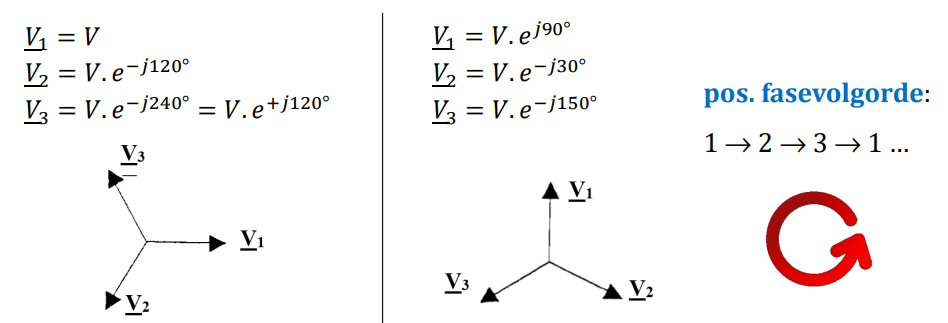
\includegraphics[width=0.8\textwidth]{assets/3-fase.png}
    \caption{Driefasig spanningssysteem dat de drie fasen toont met een faseverschil van 120 graden tussen elke fase.}
    \label{fig:3-fase.png}
\end{figure}

\begin{figure}[ht]
    \centering
    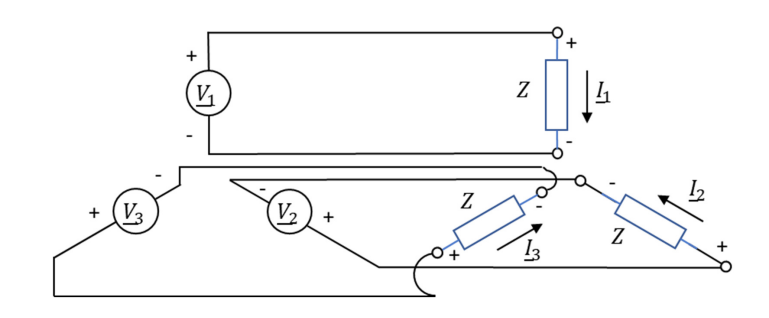
\includegraphics[width=0.45\textwidth]{assets/circuit3-fase.png}
    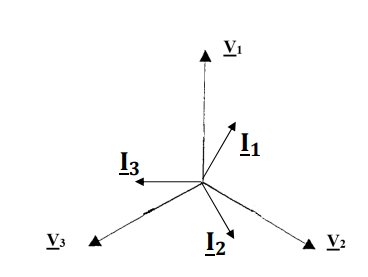
\includegraphics[width=0.45\textwidth]{assets/fasors3fase.png}
    \caption{Driefasig circuit met drie fasen die elk 120 graden uit fase zijn.}
    \label{fig:circuit3-fase.png}
\end{figure}
\FloatBarrier

Of de stroom voor- of naijlt op de spanning, hangt af van de belasting. In de figuur ijlt de
stroom \emph{na}, dus de belasting is inductief.
\newline

Zo'n systeem met drie losse bronnen heeft zes draden nodig. Hoe krijgen we dat aantal omlaag?
\textbf{We kunnen een ster- of driehoekconfiguratie gebruiken.}

\subsection{Sterconfiguratie}

\begin{figure}[ht]
    \centering
    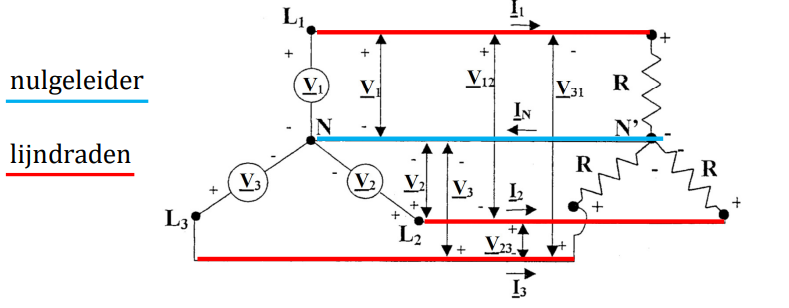
\includegraphics[width=1\textwidth]{assets/ster.png}
    \caption{Sterconfiguratie van een driefasig systeem waarbij elke fase verbonden is met een gemeenschappelijk nulpunt
        \textbf{De nulgeleider}.}
    \label{fig:ster.png}
\end{figure}

\begin{conceptbox}
    \begin{description}
        \item[Lijnspanning] $V_L$: de spanning tussen twee lijnen onderling.
        \item[Fasespanning] $V_f$: de spanning van één lijn ten opzichte van het sterpunt (de nulgeleider).
        \item[Lijnstroom] $I_L$: de stroom door een lijndraad.
        \item[Fasestroom] $I_f$: de stroom door één fase van de bron of van de belasting.
    \end{description}
\end{conceptbox}

We nemen aan dat de belasting gelijk is voor elke fase.

\subsubsection{Relatie tussen stromen en spanningen}
Omdat de belasting gelijk is voor elke fase zijn de fasestromen (de stromen door de weerstanden)
en de fasespanningen (de spanningen tegenover de nulgeleider) ook gelijk.

\[\vec{I_{L1}} = \vec{I_{f1}}\]
\[\vec{I_{L2}} = \vec{I_{F2}}\]
\[\vec{I_{L3}} = \vec{I_{F3}}\]

\[I_N = I_{f1} + I_{f2} + I_{f3}\]
Bij evenwichtige belastingen is de som van de fasestromen nul dus:
\[\vec{I_N} = 0 = I_{f1}+ I_{f2} + I_{f3}\]

\begin{wrapfigure}{r}{0.4\textwidth}
    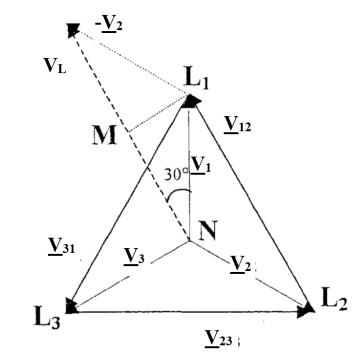
\includegraphics[width=0.4\textwidth]{assets/fasors.png}
\end{wrapfigure}


Deze figuur lijkt eerst verwarrend maar het geeft ons de
relaties tussen de spanningen.
Dit zijn de fasors van de bronspanningen met de lijnspanningen.
We weten uit het schema dat:
\[V_{12} = V_{1} - V_{2}\]
\[V_{23} = V_{2} - V_{3}\]
\[V_{31} = V_{3} - V_{1}\]


\textbf{Waar komt $\sqrt{3}$ vandaan?} $M\!N$ is de helft van de lijnspanning:
\[2\,M\!N = V_{L1} \qquad\text{met}\qquad M\!N = V_{f1}\cos(30^\circ)\]
\[V_{L1} = 2 V_{f1} \cos(30^\circ) = \sqrt{3}\, V_{f1}\]


\textbf{En waar komt de $30^\circ$ vandaan?} De twee fasespanningen liggen $120^\circ$ uit
elkaar. Trek je twee even lange vectoren onder $120^\circ$ van elkaar af, dan ligt het
resultaat precies \textbf{in het midden} tussen beide --- dus $60^\circ$ van elk. Ten
opzichte van $V_{f1}$ zelf is dat een draaiing van $30^\circ$.
\[\vec{V}_L = \sqrt{3}\,\vec{V}_f \angle 30^\circ\]
De $120^\circ$ is dus de hoek \emph{tussen de fasespanningen}; de lijnspanning zelf is maar
$30^\circ$ gedraaid.


Deze relaties gelden alleen voor \textbf{evenwichtige belastingen}.
\frm{Relatie lijn- en fasespanning \& stromen in sterconfiguratie}
{\vec{V_L} = \sqrt{3} \cdot \vec{V_f}\angle 30^\circ \quad , \quad \vec{I_L} = \vec{I_f}}
{Met $\vec{V_L}$ de lijnspanning in Volt, $\vec{V_f}$ de fasespanning in Volt,
    $\vec{I_L}$ de lijnstroom in Ampère en $\vec{I_f}$ de fasestroom in Ampère.}

In de voorbeelden hieronder kijken we enkel naar de \emph{groottes}; de hoekverschuiving van
$30^\circ$ laten we weg omdat er niets mee gevraagd wordt. Zodra je met vermogens of fasehoeken
rekent, moet ze er wél bij.

Voorbeeld: Je hebt een 3-fase stersysteem met een fasespanning van $230 V$.
Wat is de lijnspanning?
\[\vec{V_L} = \sqrt{3} \cdot \vec{V_f} = \sqrt{3} \cdot 230 V = 398.37 V\]


Nog een voorbeeld: Je hebt een 3-fase stersysteem met een lijnstroom van $10 A$.
Wat is de fasestroom?
\[\vec{I_L} = \vec{I_f} = 10 A\]


Nog een laatste: Je hebt een 3-fase stersysteem met een lijnspanning van $400 V$. Je hebt een fasestroom van $5\,\text{A}\angle 30^\circ$.
Wat is de fasespanning? Wat is de lijnstroom? De impedantie van elke fase?
\[\vec{V_L} = 400 V\]
\[\vec{V_f} = \frac{\vec{V_L}}{\sqrt{3}} = \frac{400 V}{\sqrt{3}} = 230.94 V\]
\[\vec{I_L} = \vec{I_f} = 5\,\text{A}\angle 30^\circ\]
\[\vec{Z_f} = \frac{\vec{V_f}}{\vec{I_f}} = \frac{230.94\,\text{V}}{5\,\text{A}\angle 30^\circ} = 46.19 \angle -30^\circ\ \Omega = 40 - j23.09\ \Omega\]


\subsection{Driehoekconfiguratie}
Bij een driehoekconfiguratie zijn de belastingen en bronnen verbonden in een driehoek.

Snelle herhaling van de definities:
\begin{conceptbox}
    \begin{description}
        \item[Lijnspanning] $V_L$: de spanning tussen twee lijnen onderling.
        \item[Fasespanning] $V_f$: de spanning over één tak van de driehoek. Hier is er geen
              sterpunt, dus $V_f = V_L$.
        \item[Lijnstroom] $I_L$: de stroom door een lijndraad.
        \item[Fasestroom] $I_f$: de stroom door één tak van de driehoek.
    \end{description}
\end{conceptbox}

\begin{figure}[ht]
    \centering
    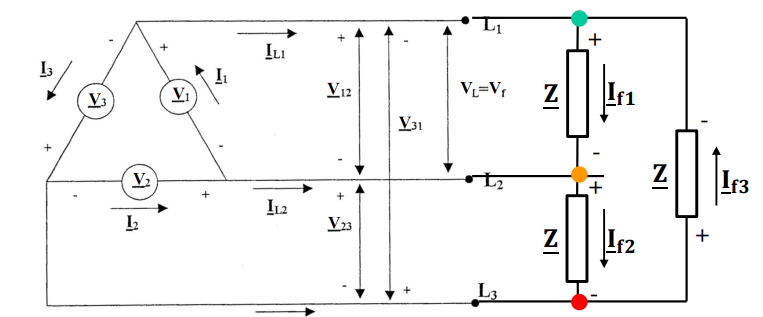
\includegraphics[width=1\textwidth]{assets/driehoek 3fasesyteem.png}
    \caption{Driehoekconfiguratie van een driefasig systeem.}
    \label{fig:driehoek 3fasesyteem.png}
\end{figure}

Elke bron staat hier rechtstreeks tussen twee lijnen. De fasespanning \emph{is} dus de
lijnspanning:
\[\vec{V_{L1}} = \vec{V_{f1}}\]
\[\vec{V_{L2}} = \vec{V_{f2}}\]
\[\vec{V_{L3}} = \vec{V_{f3}}\]

Zijn de belastingen gelijk, dan loopt er \textbf{geen circulatiestroom} rond in de driehoek
zelf: de drie bronspanningen heffen elkaar op ($\vec{V}_1 + \vec{V}_2 + \vec{V}_3 = 0$), dus er is
geen netto spanning die zo'n stroom kan drijven.

Als we de wet van Kirchhoff toepassen op de knooppunten krijgen we:
\[\vec{I_{L1}} = \vec{I_{f1}} - \vec{I_{f3}}\]
\[\vec{I_{L2}} = \vec{I_{f2}} - \vec{I_{f1}}\]
\[\vec{I_{L3}} = \vec{I_{f3}} - \vec{I_{f2}}\]

Analoog aan de sterconfiguratie maar nu voor de stromen:

Deze relaties gelden alleen voor \textbf{evenwichtige belastingen}.

\frm{Relatie lijn- en fasestromen \& spanningen in driehoekconfiguratie}
{\vec{I_L} = \sqrt{3} \cdot \vec{I_f}\angle -30^\circ \quad , \quad \vec{V_L} = \vec{V_f}}
{Met $\vec{I_L}$ de lijnstroom in Ampère, $\vec{I_f}$ de fasestroom in Ampère,
    $\vec{V_L}$ de lijnspanning in Volt en $\vec{V_f}$ de fasespanning in Volt.}

\begin{waarschuwing}[De 30 graden zijn geen detail]
    De factor $\sqrt{3}$ onthoudt iedereen, de \textbf{hoekverschuiving van $30^\circ$} niet.
    Vergeet je die, dan zit je $30^\circ$ fout op je fasehoek, en dus op je arbeidsfactor en je
    vermogens.

    \textbf{Waar komt die $30^\circ$ vandaan?} De lijnstroom is het \emph{verschil} van twee
    fasestromen die $120^\circ$ uit elkaar liggen. Trek je twee even lange vectoren onder
    $120^\circ$ van elkaar af, dan is het resultaat $\sqrt{3}$ keer zo lang en $30^\circ$ gedraaid.
    Teken het één keer en je vergeet het nooit meer.

    Reken het desnoods na met KCL in hoekpunt $A$, met $\underline{I}_{AB} = I_f\angle 0^\circ$ als
    referentie en $\underline{I}_{CA} = I_f\angle 120^\circ$:
    \[\underline{I}_A = \underline{I}_{AB} - \underline{I}_{CA}
        = I_f\left(1\angle 0^\circ - 1\angle 120^\circ\right)
        = I_f\left[(1 + j0) - \left(-\tfrac{1}{2} + j\tfrac{\sqrt3}{2}\right)\right]
        = I_f\left(\tfrac{3}{2} - j\tfrac{\sqrt3}{2}\right)\]
    Die laatste factor heeft grootte $\sqrt{(3/2)^2 + (\sqrt3/2)^2} = \sqrt{3}$ en hoek
    $\arctan\frac{-\sqrt3/2}{3/2} = -30^\circ$, dus
    $\underline{I}_A = \sqrt3\,I_f\angle -30^\circ$. De $\sqrt3$ en de $30^\circ$ komen dus uit
    dezelfde ene aftrekking --- daarom kan je ze ook niet los van elkaar onthouden.

    \textbf{Het teken hangt af van de fasevolgorde:}
    \begin{itemize}
        \item positieve volgorde ($abc$): $\vec{I_L} = \sqrt{3}\,\vec{I_f}\angle -30^\circ$ en
              $\vec{V_L} = \sqrt{3}\,\vec{V_f}\angle +30^\circ$;
        \item negatieve volgorde ($acb$): beide tekens draaien om.
    \end{itemize}
    Op het examen staat de volgorde er altijd bij --- lees ze.
\end{waarschuwing}

\begin{figure}[ht]
    \centering
    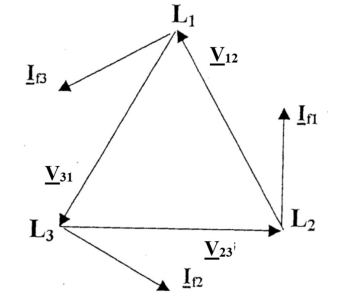
\includegraphics[width=0.4\textwidth]{assets/fasorsindriehoek.png}
    
\includegraphics[width=0.4\textwidth]{assets/image4.png}
    \caption{Fasordiagram van de driehoekconfiguratie: relatie tussen lijn- en fasestromen.}
    \label{fig:fasorsindriehoek.png}
\end{figure}

\subsection{Omzetting ster- naar driehoekconfiguratie}

Je kunt een sterconfiguratie omzetten naar een driehoekconfiguratie en omgekeerd. Bij een
\textbf{evenwichtige} last is dat één simpele factor 3; bij een onevenwichtige last heb je de
algemene formules verderop nodig.

\frm{Delta naar Ster en omgekeerd}{\underline{Z}_Y = \frac{\underline{Z}_\Delta}{3} \quad , \quad \underline{Z}_\Delta = 3\,\underline{Z}_Y}{Met $\underline{Z}_Y$ de impedantie van de equivalente
    Y-verbonden belasting in Ohm en $\underline{Z}_\Delta$ de impedantie van de $\Delta$-verbonden belasting in Ohm.}

\textbf{Waarom precies een factor 3?} Het idee achter elke ster-driehoekomzetting is dit: de twee
schakelingen moeten van \emph{buitenaf} niet te onderscheiden zijn. Meet je tussen twee klemmen,
dan moet je in beide gevallen dezelfde impedantie zien. Voor een evenwichtige last volstaat één
zo'n meting.

\stapreden{\textbf{Ster.} Meet je tussen klem 1 en klem 2, dan loop je via het sterpunt door twee takken in serie (de derde tak hangt er los bij en trekt geen stroom):}
\[\underline{Z}_{12,Y} = \underline{Z}_Y + \underline{Z}_Y = 2\,\underline{Z}_Y\]

\stapreden{\textbf{Driehoek.} Tussen dezelfde twee klemmen zie je nu de tak 1--2 rechtstreeks, parallel met de twee andere takken die samen in serie staan:}
\[\underline{Z}_{12,\Delta} = \underline{Z}_\Delta \parallel \left(\underline{Z}_\Delta + \underline{Z}_\Delta\right)
    = \frac{\underline{Z}_\Delta \cdot 2\underline{Z}_\Delta}{\underline{Z}_\Delta + 2\underline{Z}_\Delta}
    = \frac{2\underline{Z}_\Delta^2}{3\underline{Z}_\Delta} = \frac{2}{3}\,\underline{Z}_\Delta\]

\stapreden{Beide gelijkstellen:}
\[2\,\underline{Z}_Y = \frac{2}{3}\,\underline{Z}_\Delta
    \qquad\Longrightarrow\qquad
    \boxed{\underline{Z}_\Delta = 3\,\underline{Z}_Y}\]

Dat verklaart meteen ook de ster-driehoekstarter: schakel dezelfde motorwikkelingen van ster naar
driehoek en hun impedantie wordt drie keer kleiner, dus trekken ze drie keer meer stroom en drie
keer meer vermogen. In ster start de motor zacht, in driehoek draait hij op vol vermogen.

Als de belastingen niet evenwichtig zijn, moet je de volgende formules gebruiken (die volgen uit
precies dezelfde eis, maar dan voor alle drie de klemmenparen tegelijk):


\begin{figure}[ht]
    \centering
    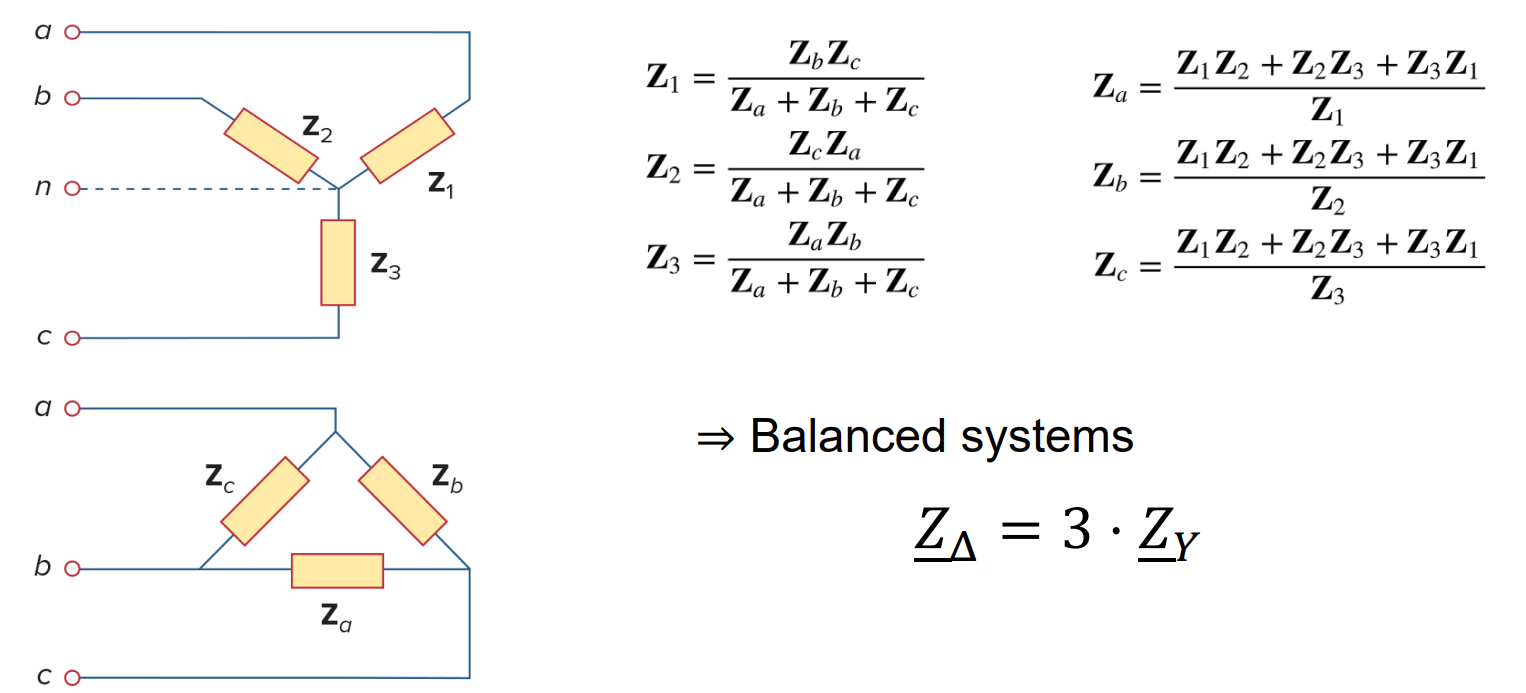
\includegraphics[width=0.8\textwidth]{assets/omzettingster en driehoek.png}
    \caption{Omzetting ster- naar driehoekconfiguratie en omgekeerd.}
    \label{fig:omzettingster en driehoek.png}
\end{figure}

Noem de drie \emph{driehoek}impedanties $Z_1$, $Z_2$ en $Z_3$, en de drie bijhorende
\emph{ster}impedanties $Z_a$, $Z_b$ en $Z_c$.

\frm{Omzetting driehoek- naar sterconfiguratie}
{Z_a = \frac{Z_{1} Z_{3}}{Z_{1} + Z_{2} + Z_{3}} \quad , \quad
    Z_b = \frac{Z_{1} Z_{2}}{Z_{1} + Z_{2} + Z_{3}} \quad , \quad
    Z_c = \frac{Z_{2} Z_{3}}{Z_{1} + Z_{2} + Z_{3}}}
{Met $Z_a, Z_b, Z_c$ de sterimpedanties in $\Omega$ en $Z_1, Z_2, Z_3$ de driehoekimpedanties in
    $\Omega$. Ezelsbruggetje: in de teller staat het \textbf{product van de twee driehoektakken die
        aan dat sterpunt raken}, in de noemer de \textbf{som van alle drie}.}

\frm {Omzetting ster- naar driehoekconfiguratie}
{Z_{1} = \frac{Z_{a} Z_{b} + Z_{b} Z_{c} + Z_{c} Z_{a}}{Z_{c}} \quad , \quad
    Z_{2} = \frac{Z_{a} Z_{b} + Z_{b} Z_{c} + Z_{c} Z_{a}}{Z_{a}} \quad , \quad
    Z_{3} = \frac{Z_{a} Z_{b} + Z_{b} Z_{c} + Z_{c} Z_{a}}{Z_{b}}}
{Met dezelfde symbolen. De teller is telkens \emph{dezelfde} som; enkel de noemer wisselt: de
    sterimpedantie die \textbf{tegenover} die driehoektak ligt.}

\begin{examenbox}
    Is de belasting \textbf{evenwichtig}, dan vereenvoudigen beide formules tot
    \[Z_\Delta = 3 Z_Y\]
    en dat is de vorm die je op het examen bijna altijd nodig hebt. De algemene formules hierboven
    heb je enkel bij een \emph{ongebalanceerde} last.
\end{examenbox}



Hieronder een voorbeeld oefening uitgewerkt.
\begin{figure}[ht]
    \centering
    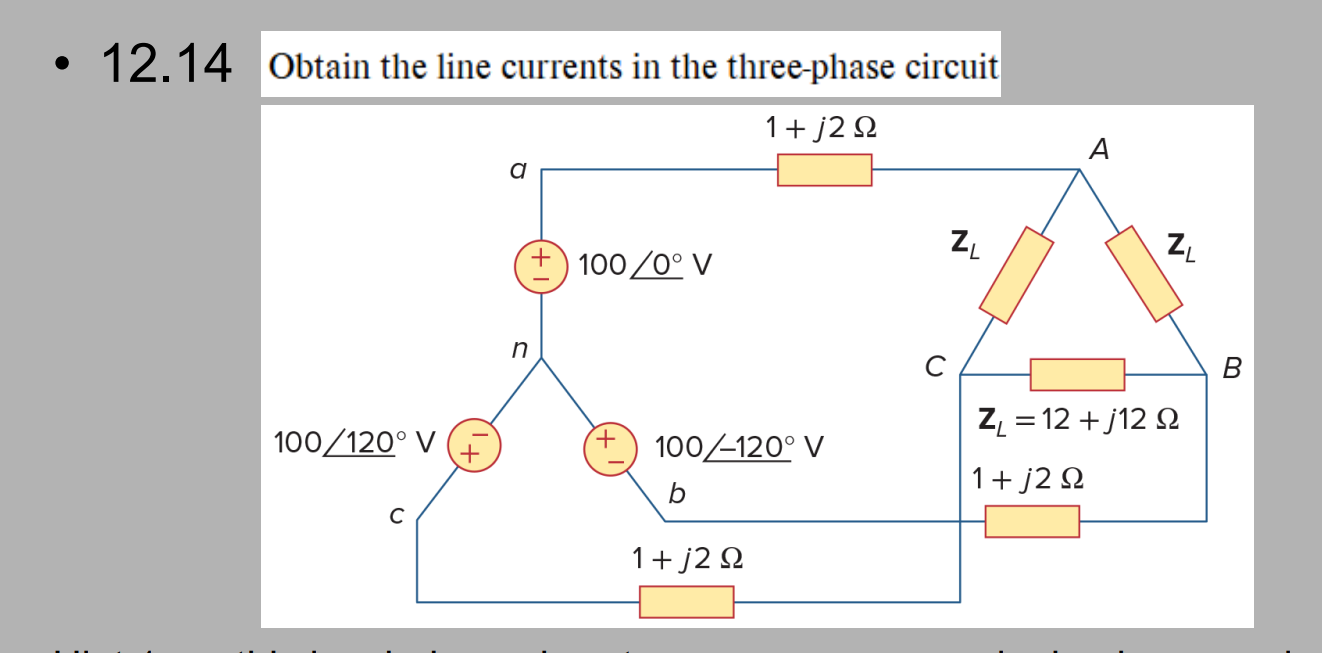
\includegraphics[width=0.8\textwidth]{assets/vboefening.png}
    \caption{Schema van het 3-fase systeem met transmissielijn en Delta-belasting uit de voorbeeldoefening.}
    \label{fig:vboefening.png}
\end{figure}
\FloatBarrier
\begin{oefenblok}


    \textbf{Uitgewerkt voorbeeld: 3-fase systeem met transmissielijn en Delta-belasting}

    We hebben een evenwichtig 3-fase systeem met de volgende kenmerken:

    \begin{description}
        \item[Bron]: Evenwichtige Y-verbonden bron met positieve fasevolgorde (abc)
              \begin{align*}
                  \vec{V}_{an} & = 100\angle{0^\circ} \text{ V}    \\
                  \vec{V}_{bn} & = 100\angle{-120^\circ} \text{ V} \\
                  \vec{V}_{cn} & = 100\angle{120^\circ} \text{ V}
              \end{align*}
        \item[Lijnimpedantie]: $\vec{Z}_{\text{lijn}} = 1 + j2 \text{ } \Omega$ per fase
        \item[Belasting]: Evenwichtige $\Delta$-verbonden belasting met $\vec{Z}_{\Delta} = 12 + j12 \text{ } \Omega$ per fase
    \end{description}

    \textbf{Stap 1: Delta-belasting omzetten naar equivalente Ster-belasting}

    Voor een evenwichtige belasting is de impedantie van de equivalente Y-verbonden belasting ($\vec{Z}_Y$)
    één derde van de $\Delta$-verbonden belasting impedantie ($\vec{Z}_\Delta$):

    $$\vec{Z}_Y = \frac{\vec{Z}_\Delta}{3} = \frac{12 + j12}{3} = 4 + j4 \text{ } \Omega$$

    \textbf{Stap 2: Eenfase equivalent circuit analyseren (fase 'a')}

    Nu kunnen we het eenfase equivalent circuit voor fase 'a' analyseren. Dit bestaat uit de bronspanning $\vec{V}_{an}$
    in serie met de lijnimpedantie $\vec{Z}_{\text{lijn}}$ en de equivalente belastingsimpedantie $\vec{Z}_Y$.

    \textbf{Bereken de totale impedantie per fase:}

    Omdat $\vec{Z}_{\text{lijn}}$ en $\vec{Z}_Y$ in serie staan:

    $$\vec{Z}_{\text{totaal}} = \vec{Z}_{\text{lijn}} + \vec{Z}_Y = (1 + j2) + (4 + j4) = 5 + j6 \text{ } \Omega$$

    \textbf{Omzetten naar poolcoördinaten:}

    \begin{align*}
        |\vec{Z}| & = \sqrt{5^2 + 6^2} = \sqrt{61} \approx 7.81 \text{ } \Omega \\
        \theta    & = \tan^{-1}\left(\frac{6}{5}\right) \approx 50.19^\circ
    \end{align*}

    $$\vec{Z}_{\text{totaal}} \approx 7.81\angle{50.19^\circ} \text{ } \Omega$$

    \textbf{Stap 3: Bereken lijnstroom $\vec{I}_a$}

    Met behulp van de wet van Ohm voor het eenfase equivalent circuit:

    $$\vec{I}_a = \frac{\vec{V}_{an}}{\vec{Z}_{\text{totaal}}} = \frac{100\angle{0^\circ}}{7.81\angle{50.19^\circ}} = 12.80\angle{-50.19^\circ} \text{ A}$$

    \textbf{Stap 4: Bepaal $\vec{I}_b$ en $\vec{I}_c$}

    Omdat het systeem evenwichtig is met positieve fasevolgorde (abc), hebben de lijnstromen dezelfde magnitude
    (12.80 A) maar zijn ze faseverschoven met $-120^\circ$ en $+120^\circ$ ten opzichte van $\vec{I}_a$:

    $$\vec{I}_b = 12.80\angle{-50.19^\circ - 120^\circ} = 12.80\angle{-170.19^\circ} \text{ A}$$

    $$\vec{I}_c = 12.80\angle{-50.19^\circ + 120^\circ} = 12.80\angle{69.81^\circ} \text{ A}$$
    \textbf{Eindantwoord}

    De drie lijnstromen zijn:

    \begin{align*}
        \vec{I}_a & = 12.80\angle{-50.19^\circ} \text{ A}  \\
        \vec{I}_b & = 12.80\angle{-170.19^\circ} \text{ A} \\
        \vec{I}_c & = 12.80\angle{69.81^\circ} \text{ A}
    \end{align*}
\end{oefenblok}

\begin{figure}[ht]
    \centering
    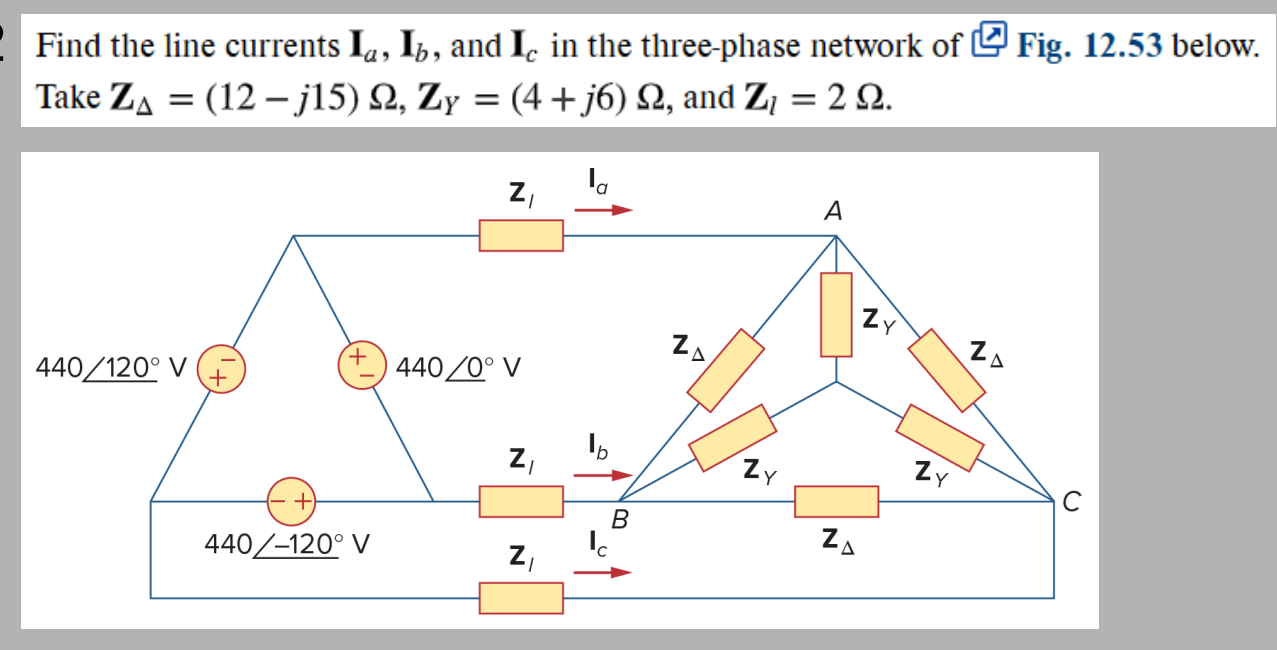
\includegraphics[width=0.8\textwidth]{assets/vboef.png}
    \caption{Schema van het 3-fase systeem met Delta-bron en gemengde Ster/Delta-belasting uit de voorbeeldoefening.}
    \label{fig:vboef.png}
\end{figure}


\begin{oefenblok}

    \begin{description}
        \item[Bron]: Delta-verbonden bron met $\vec{V}_{ab} = 440\angle{0^\circ}$ V. Dit is positieve fasevolgorde (abc).
        \item[Lijnimpedantie]: $\vec{Z}_l = 2 \text{ } \Omega$
        \item[Belastingen]:
              \begin{itemize}
                  \item Belasting 1 (Ster): $\vec{Z}_Y = 4 + j6 \text{ } \Omega$
                  \item Belasting 2 (Delta): $\vec{Z}_\Delta = 12 - j15 \text{ } \Omega$
              \end{itemize}
    \end{description}

    \textbf{Strategie}: We zetten het hele circuit om naar een eenfase equivalent. Daarvoor moeten we de Delta-bron omzetten naar een Ster-bron en de Delta-belasting naar een Ster-belasting.

    \textbf{Stap 1: Delta-belasting omzetten naar equivalente Ster-belasting}

    We gebruiken de "Deel door 3" regel om de Delta-belasting ($\vec{Z}_\Delta$) om te zetten naar een equivalente Ster-belasting ($\vec{Z}_{\Delta \to Y}$):

    $$\vec{Z}_{\Delta \to Y} = \frac{\vec{Z}_\Delta}{3} = \frac{12 - j15}{3} = 4 - j5 \text{ } \Omega$$

    Nu hebben we aan de belastingskant effectief twee Ster-impedanties in parallel:
    \begin{itemize}
        \item Originele $\vec{Z}_Y = 4 + j6 \text{ } \Omega$
        \item Omgezette $\vec{Z}_{\Delta \to Y} = 4 - j5 \text{ } \Omega$
    \end{itemize}

    \textbf{Stap 2: Bereken de equivalente belastingsimpedantie ($\vec{Z}_p$)}

    Omdat deze twee equivalente Ster-belastingen in parallel staan, gebruiken we de product-over-som formule:

    $$\vec{Z}_p = \frac{\vec{Z}_Y \cdot \vec{Z}_{\Delta \to Y}}{\vec{Z}_Y + \vec{Z}_{\Delta \to Y}}$$

    \textbf{Teller (Product):}
    $$(4+j6)(4-j5) = 16 - j20 + j24 + 30 = 46 + j4$$

    \textbf{Noemer (Som):}
    $$(4+j6) + (4-j5) = 8 + j1$$

    \textbf{Deling:}
    $$\vec{Z}_p = \frac{46 + j4}{8 + j1}$$

    Vermenigvuldig boven en onder met de geconjugeerde ($8 - j1$):

    $$\vec{Z}_p = \frac{(46 + j4)(8 - j1)}{(8 + j1)(8 - j1)} = \frac{368 - j46 + j32 + 4}{65} = \frac{372 - j14}{65}$$

    $$\vec{Z}_p \approx 5.723 - j0.215 \text{ } \Omega$$

    \textbf{Stap 3: Zet de bron om naar Ster}

    Het probleem geeft de lijnspanning $\vec{V}_{ab} = 440\angle{0^\circ}$ V. Voor het eenfase equivalent hebben we de fase-naar-nul spanning $\vec{V}_{an}$.

    Bij positieve fasevolgorde is de fasespanningsgrootte gedeeld door $\sqrt{3}$, en de hoek verschoven met $-30^\circ$:

    $$\vec{V}_{an} = \frac{440}{\sqrt{3}}\angle{(0^\circ - 30^\circ)} \approx 254.03\angle{-30^\circ} \text{ V}$$
    \textbf{Stap 4: Bereken totale impedantie en lijnstroom $\vec{I}_a$}

    Nu hebben we een simpele lus met bronspanning $\vec{V}_{an}$, lijnimpedantie $\vec{Z}_l$ en equivalente belastingsimpedantie $\vec{Z}_p$.

    \textbf{Totale impedantie:}
    $$\vec{Z}_{totaal} = \vec{Z}_l + \vec{Z}_p = 2 + (5.723 - j0.215) = 7.723 - j0.215 \text{ } \Omega$$

    \textbf{Omzetten naar poolcoördinaten:}

    Magnitude: $\sqrt{7.723^2 + 0.215^2} \approx 7.726$

    Hoek: $\tan^{-1}\left(\frac{-0.215}{7.723}\right) \approx -1.59^\circ$

    $$\vec{Z}_{totaal} = 7.726\angle{-1.59^\circ} \text{ } \Omega$$

    \textbf{Bereken $\vec{I}_a$ met wet van Ohm:}

    $$\vec{I}_a = \frac{\vec{V}_{an}}{\vec{Z}_{totaal}} = \frac{254.03\angle{-30^\circ}}{7.726\angle{-1.59^\circ}}$$

    $$\vec{I}_a = 32.88\angle{(-30^\circ - (-1.59^\circ))} = 32.88\angle{-28.41^\circ} \text{ A}$$

    \textbf{Stap 5: Bepaal $\vec{I}_b$ en $\vec{I}_c$}

    Pas de $120^\circ$ faseverschuiving toe voor een evenwichtig positief systeem:
    $$\vec{I}_a = 32.88\angle{-28.41^\circ} \text{ A}$$

    $$\vec{I}_b = 32.88\angle{(-28.41^\circ - 120^\circ)} = 32.88\angle{-148.41^\circ} \text{ A}$$

    $$\vec{I}_c = 32.88\angle{(-28.41^\circ + 120^\circ)} = 32.88\angle{91.59^\circ} \text{ A}$$

    \textbf{Samenvatting van de stappen}

    \begin{enumerate}
        \item Zet $\Delta$-belasting om naar Y-belasting (deel door 3)
        \item Combineer parallelle belastingen (product over som)
        \item Zet bronlijnspanning om naar fasespanning (deel door $\sqrt{3}$, verschuif $-30^\circ$)
        \item Tel lijnimpedantie op
        \item Gebruik wet van Ohm
    \end{enumerate}

\end{oefenblok}






\subsection{3-fase vermogen}

In een 3-fase systeem is het totale vermogen de som van de vermogens in elke fase.
\newline
\textbf{Belangrijk:} in de vermogensformules is $\phi$ de fasehoek \textbf{tussen spanning en stroom van de belasting} (arbeidsfactorhoek / impedantiehoek). Dit is \textbf{niet} het $120^\circ$ faseverschil tussen de drie bronspanningen.
\frm{Totaal vermogen in 3-fase systeem}{P_{totaal} = \sum_{n=1}^{3} P_{fase} = 3 \cdot P_{fase}}
{Met $P_{totaal}$ het totale actieve vermogen in Watt en $P_{fase}$ het actieve vermogen per fase in Watt.}


met gelijke belastingen in elke fase:
\[P_{totaal} = 3 \cdot P_{fase}\]
Met het vermogen per fase:
\frm{Vermogen per fase in 3-fase systeem}{P_{fase} = V_f \cdot I_f \cdot \cos \phi}
{Met $P_{fase}$ het actieve vermogen per fase in Watt, $V_f$ de fasespanning in Volt,
    $I_f$ de fasestroom in Ampère en $\phi$ de fasehoek tussen $V_f$ en $I_f$ (dus tussen spanning en stroom van de belasting) in graden of radialen.}

Als we de relaties tussen lijn- en fasespanningen voor ster- en driehoekconfiguraties invullen krijgen we:

\begin{figure}[ht]
    \centering
    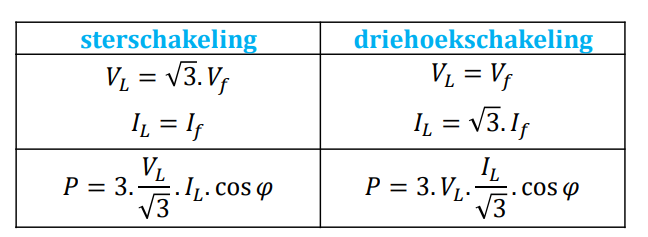
\includegraphics[width=0.8\textwidth]{assets/totaalvermogen.png}
    \caption{Totaal vermogen in een 3-fase systeem voor zowel ster- als driehoekconfiguraties. In beide gevallen is het totale actieve vermogen $P_{totaal} = \sqrt{3} V_L I_L \cos \phi$, waarbij $\phi$ de fasehoek is tussen spanning en stroom van de belasting (arbeidsfactorhoek), niet het $120^\circ$ faseverschil tussen de fasen.}
    \label{fig:totaalvermogen.png}
\end{figure}

\frm{Totaal vermogen in 3-fase systeem}{P_{totaal} = \sqrt{3} V_L \cdot I_L \cdot \cos \phi}
{Met $P_{totaal}$ het totale actieve vermogen in Watt, $V_L$ de lijnspanning in Volt,
    $I_L$ de lijnstroom in Ampère en $\phi$ de fasehoek tussen spanning en stroom van de belasting (arbeidsfactorhoek) in graden of radialen.}


\subsection{2-wattmethode}
Bij gelijke belastingen is het totale vermogen simpelweg $P_{totaal} = 3 \cdot P$.
Zijn de belastingen niet gelijk, dan kunnen we het totale vermogen niet meer op die manier berekenen
en gebruiken we in plaats daarvan de 2-wattmethode.

De voor de hand liggende aanpak zou zijn: \'e\'en wattmeter per fase, alle drie gemeten tegenover
hetzelfde referentiepunt $O$, en dan $P_{totaal} = P_1 + P_2 + P_3$. Dat werkt altijd, maar het kan
met \'e\'en meter minder --- en dat is precies wat de 2-wattmethode doet.

\begin{figure}[H]
    \centering
    \begin{tikzpicture}[
        wm/.style={draw=schoolBlue!80, fill=schoolBlue!8, line width=0.8pt,
                   minimum width=9mm, minimum height=6mm, inner sep=0pt, font=\scriptsize\bfseries},
        last/.style={draw, thick, minimum width=17mm, minimum height=25mm, align=center,
                     font=\scriptsize},
        spoel/.style={schoolRed, thick, dashed}
      ]
      % ================= drie wattmeters =================
      \begin{scope}
        \node[font=\footnotesize\bfseries, anchor=south] at (2.4,2.85) {drie wattmeters};
        \foreach \y/\lbl/\w/\sx in {2.2/$L_1$/W$_1$/1.10, 1.3/$L_2$/W$_2$/1.40, 0.4/$L_3$/W$_3$/1.70} {
            \draw (0.15,\y) node[left, font=\scriptsize] {\lbl} -- (0.95,\y);
            \node[wm] at (1.4,\y) {\w};
            \draw (1.85,\y) -- (3.3,\y);
            \draw[spoel] (\sx,{\y-0.30}) -- (\sx,-0.55);
        }
        \draw[spoel] (1.10,-0.55) -- (1.70,-0.55);
        \node[circle, fill=schoolRed, inner sep=1.3pt] at (1.40,-0.55) {};
        \node[font=\scriptsize, schoolRed, below] at (1.40,-0.68) {$O$};
        \node[last, anchor=west] at (3.3,1.3) {driefasige\\last\\(willekeurig)};
        \node[font=\scriptsize, anchor=north, align=center] at (2.4,-1.15)
             {$P_{tot} = P_1 + P_2 + P_3$\\\emph{werkt altijd}};
      \end{scope}
      % ================= twee wattmeters =================
      \begin{scope}[shift={(7.6,0)}]
        \node[font=\footnotesize\bfseries, anchor=south] at (2.4,2.85) {twee wattmeters};
        \draw (0.15,2.2) node[left, font=\scriptsize] {$L_1$} -- (0.95,2.2);
        \node[wm] at (1.4,2.2) {W$_1$};
        \draw (1.85,2.2) -- (3.3,2.2);
        \draw (0.15,1.3) node[left, font=\scriptsize] {$L_2$} -- (3.3,1.3);
        \draw (0.15,0.4) node[left, font=\scriptsize] {$L_3$} -- (0.95,0.4);
        \node[wm] at (1.4,0.4) {W$_2$};
        \draw (1.85,0.4) -- (3.3,0.4);
        \draw[spoel] (1.40,1.90) -- (1.40,1.30);
        \draw[spoel] (1.40,0.70) -- (1.40,1.30);
        \node[circle, fill=schoolRed, inner sep=1.3pt] at (1.40,1.30) {};
        \node[last, anchor=west] at (3.3,1.3) {driefasige\\last\\(willekeurig)};
        \node[font=\scriptsize, anchor=north, align=center] at (2.4,-1.15)
             {$P_{tot} = P_1 + P_2$\\\emph{drie draden, ook bij onevenwicht}};
      \end{scope}
      % legende
      \node[font=\scriptsize, anchor=north, align=center] at (5.0,-2.05)
           {\textcolor{schoolRed}{\rule[0.35ex]{4mm}{0.6pt}\hspace{0.6mm}\rule[0.35ex]{2mm}{0.6pt}}\;
            = spanningsspoel (meet t.o.v.\ de referentie)};
    \end{tikzpicture}
    \caption{Links de voor de hand liggende aanpak: \'e\'en wattmeter per lijn, en alle drie de
        spanningsspoelen naar hetzelfde punt $O$. Rechts de 2-wattmethode: de stroomspoelen zitten in
        twee lijnen, en de derde lijn ($L_2$) is de gemeenschappelijke referentie voor beide
        spanningsspoelen. Die derde lijn krijgt dus \emph{geen} wattmeter --- dat is de hele
        besparing.}
    \label{fig:wattmeters-2-vs-3}
\end{figure}
\FloatBarrier
\FloatBarrier

\begin{waarschuwing}[Wanneer twee wattmeters níet volstaan]
    De 2-wattmethode werkt bij \textbf{drie draden}: een driehoek, of een ster \emph{zonder}
    nulgeleider. Ze werkt ook bij onevenwicht --- dat is juist haar sterkte.

    Ze werkt \belangrijk{niet} zodra er een \textbf{nulgeleider is waar stroom door loopt}
    (vierdraads en onevenwichtig). De afleiding steunt erop dat $\underline{I}_1 + \underline{I}_2 +
    \underline{I}_3 = 0$, en die som is dan niet meer nul. In dat geval heb je wel degelijk
    \textbf{drie} wattmeters nodig.
\end{waarschuwing}

\begin{figure}[ht]
    \centering
    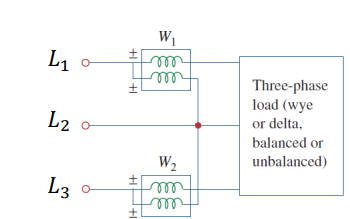
\includegraphics[width=0.6\textwidth]{assets/2-wattmethode.png}
    \caption{2-wattmethode voor het meten van het totale actieve vermogen in een 3-fase systeem met ongelijke belastingen. Door twee wattmeters aan te sluiten op specifieke lijnen, kunnen we het totale vermogen berekenen als $P_{totaal} = P_1 + P_2$.}
    \label{fig:2-wattmethode.png}
\end{figure}
\FloatBarrier

\frm{2-wattmethode}{P_{totaal} = P_1 + P_2}{Met $P_{totaal}$ het totale actieve vermogen in Watt, $P_1$ het vermogen gemeten door wattmeter 1 in Watt en $P_2$ het vermogen gemeten door wattmeter 2 in Watt.}

De wattmeters meten de fasestroom en de lijnspanning.

\[P_1 = V_{12} \cdot I_{f1} \cdot \cos (30^\circ + \phi_1) = V_L \cdot I_L \cdot \cos (30^\circ + \phi_1)\]
\[V_{23} = -V_{32}\]
$V_{32}$ ijlt achter op $V_{3}$ met 30 graden
\[P_2 = V_{32} \cdot I_{f3} \cdot \cos (-30^\circ + \phi_3) = V_L \cdot I_L \cdot \cos (-30^\circ + \phi_3)\]

\begin{figure}[ht]
    \centering
    
\includegraphics[width=0.45\textwidth]{assets/image5.png}
    
\includegraphics[width=0.45\textwidth]{assets/image6.png}
    \caption{Fasordiagrammen bij de afleiding van de 2-wattmethode.}
    \label{fig:image5.png}
\end{figure}

\begin{examenbox}[EXAMENVRAAG: waarom is de nulgeleider misleidend?]
    Omdat men er te makkelijk van uitgaat dat er ``toch geen stroom door loopt''. Dat klopt alleen
    bij een \emph{perfect} evenwichtig systeem. Zodra er onevenwicht is:
    \begin{itemize}
        \item loopt er wél stroom door de nulgeleider, en die kan zelfs groter zijn dan je verwacht;
        \item verschuift het sterpunt van de last (\textbf{centrumpuntverschuiving}) als de
              nulgeleider ontbreekt of onderbroken raakt, waardoor de ene fase te veel spanning
              krijgt en de andere te weinig;
        \item raakt de nulgeleider overbelast zonder dat iemand het merkt: er zit geen automaat op en
              er is geen zichtbare indicatie;
        \item stapelen bij niet-lineaire belastingen (schakelende voedingen, ledverlichting) de
              \textbf{harmonischen} zich juist \emph{op} in de nulgeleider in plaats van weg te
              vallen.
    \end{itemize}
\end{examenbox}

\frm{Totale vermogen in 2-wattmethode}{P_{totaal} = 3V_f \cdot I_f \cos{\theta}  =\sqrt{3} V_L \cdot I_L \cos{\theta}
}{Met $P_{totaal}$ het totale actieve vermogen in Watt, $V_L$ de lijnspanning in Volt,
    $I_f$ de fasestroom in Ampère, $V_f$ de fasespanning in Volt,
    $I_L$ de lijnstroom in Ampère en $\theta$ de hoek tussen de spanning en stroom}

Het reactief vermogen kan je ook berekenen met de 2-wattmethode.
\[Q_{totaal} = \sqrt{3}(P_2 - P_1)\]
\[Q_{totaal} = V_L \cdot I_L \cdot \cos(30^\circ + \phi_1) - V_L \cdot I_L \cdot \cos(-30^\circ + \phi_3)\]
\[Q_{totaal} = V_L \cdot I_L [\cos(30^\circ + \phi_1) - \cos(-30^\circ + \phi_3)]\]
\[Q_{totaal} = \sqrt{3} V_L \cdot I_L \sin{\theta}\]

\frm{reactief vermogen in 2-wattmethode}{Q_{totaal} = \sqrt{3}(P_2 - P_1) = \sqrt{3} V_L \cdot I_L \sin{\theta}
}{Met $Q_{totaal}$ het totale reactieve vermogen in Volt-Ampère reactief
    (VAR), $P_1$ het vermogen gemeten door wattmeter 1 in Watt en $P_2$ het vermogen gemeten door wattmeter 2 in Watt.}


\begin{waarschuwing}[Alleen $P_1+P_2$ geldt altijd]
    $P_{totaal} = P_1 + P_2$ volgt \textbf{enkel uit KCL} en geldt dus altijd: evenwichtig of
    niet, ster of driehoek.

    De formules voor $Q_{totaal}$, $\theta$ en $S$ hieronder gaan er daarentegen van uit dat de drie
    fasen \textbf{identiek} zijn. Bij een \emph{ongebalanceerde} belasting zijn ze gewoon
    ongeldig --- je krijgt er zelfs verkeerde tekens mee. Bereken $Q$ dan per tak met $Q = I_f^2 X$
    en tel op.
\end{waarschuwing}

\frm{fasehoek}{\theta = tan^{-1}\left(\frac{Q_{totaal}}{P_{totaal}}\right)= tan^{-1}\left(\frac{\sqrt{3}(P_2 - P_1)}{P_1 + P_2}\right)
}
{Met $\theta$ de gemiddelde fasehoek tussen spanning en stroom van de belastingen,
    $Q_{totaal}$ het totale reactieve vermogen in Volt-Ampère reactief (VAR) en $P_{totaal}$ het totale actieve vermogen in Watt.}

Het schijnbaar vermogen wordt berekend als volgt:

$S_{totaal} = P_{totaal} + j Q_{totaal}$

\subsubsection{Wat lees je nu precies af op een wattmeter?}

Een wattmeter heeft twee spoelen: een \textbf{stroomspoel} in serie met de lijn, en een
\textbf{spanningsspoel} tussen die lijn en de referentielijn. Hij geeft het actief vermogen dat bij
dat spanning-stroompaar hoort:

\frm{Aflezing van een wattmeter}{W = \text{Re}\{\underline{V} \cdot \underline{I}^{*}\} = |V||I|\cos(\phi_V - \phi_I)}
{Met $W$ de aflezing in W, $\underline{V}$ de spanning over de spanningsspoel in V en
    $\underline{I}$ de stroom door de stroomspoel in A.}

Bij de standaardopstelling met wattmeters in lijn $a$ en lijn $c$, en lijn $b$ als
gemeenschappelijke referentie, wordt dat:
\[W_1 = \text{Re}\{\underline{V}_{ab}\,\underline{I}_a^{*}\}
    \qquad\qquad
    W_2 = \text{Re}\{\underline{V}_{cb}\,\underline{I}_c^{*}\}\]

\begin{waarschuwing}[De klassiekste fout van het hele vak]
    $\underline{V}_{cb} = -\underline{V}_{bc}$, dus als $\underline{V}_{bc} = V_L\angle -120^\circ$,
    dan is $\underline{V}_{cb} = V_L\angle 60^\circ$ en \textbf{niet} $V_L\angle -120^\circ$.
    Elk jaar sneuvelen hier punten op.
\end{waarschuwing}

\textbf{Waarom volstaan twee wattmeters?} Zonder nulgeleider geldt
$\underline{I}_a + \underline{I}_b + \underline{I}_c = 0$, dus de derde lijnstroom bevat geen extra
informatie. Meet je twee lijnstromen ten opzichte van dezelfde referentielijn, dan zit daar alles in
wat je nodig hebt voor het \emph{totale} actief vermogen.

\textbf{Maar:} één wattmeter meet dan níet het vermogen van één fase. Alleen de \emph{som} heeft
fysische betekenis. Een negatieve aflezing is dus volkomen normaal en geen meetfout.

\begin{theorie}[Interpretatie van wattmeteraflezingen bij evenwichtig net]
    Uit $W_1 = V_L I_L \cos(30^\circ - \phi)$ en $W_2 = V_L I_L \cos(30^\circ + \phi)$ volgt:
    \begin{itemize}
        \item $\phi = 0^\circ$ ($\cos\phi = 1$, zuiver ohms): $W_1 = W_2 > 0$ (beide meters wijzen exact dezelfde positieve waarde aan).
        \item $0^\circ < \phi < 60^\circ$ ($\cos\phi > 0{,}5$): $W_1 > 0$ en $W_2 > 0$ (beide meters wijzen positief aan, met $W_1 > W_2$).
        \item $\phi = 60^\circ$ ($\cos\phi = 0{,}5$): $W_1 = P_{\text{totaal}}$ en $W_2 = 0$ (\textbf{meter 2 staat exact stil op 0 W}!).
        \item $\phi > 60^\circ$ ($\cos\phi < 0{,}5$): $W_1 > 0$ en \textbf{$W_2 < 0$} (meter 2 slaat negatief uit / wijzer slaat terug). Om de waarde af te lezen moet men de spanningsspoel ompolen; $P_{\text{totaal}}$ blijft algebraïsch $W_1 + W_2$.
        \item $\phi = 90^\circ$ ($\cos\phi = 0$, zuiver inductief/capacitief): $W_1 = -W_2 \implies P_{\text{totaal}} = 0$.
    \end{itemize}
\end{theorie}

\subsection{Ongebalanceerde systemen}

Zodra de drie impedanties niet meer gelijk zijn, vervallen bijna alle handige regels. Dit is precies
waarom de examenoefeningen zo vaak ongebalanceerd zijn.

\begin{center}
    \begin{tabular}{@{}p{62mm}p{20mm}p{28mm}@{}}
        \toprule
        \textbf{Regel}                                   & \textbf{Evenwichtig} & \textbf{Ongebalanceerd} \\
        \midrule
        Eén fase uitrekenen en $\pm120^\circ$ draaien    & ja                   & \textbf{nee}            \\
        $I_L = \sqrt{3}\,I_f\angle -30^\circ$ (driehoek) & ja                   & \textbf{nee}            \\
        $\underline{Z}_\Delta = 3\underline{Z}_Y$        & ja                   & \textbf{nee}            \\
        $\underline{I}_N = 0$ in de nulgeleider          & ja                   & \textbf{nee}            \\
        $Q_{tot} = \sqrt{3}(W_2 - W_1)$                  & ja                   & \textbf{nee}            \\
        $P_{tot} = W_1 + W_2$                            & ja                   & \textbf{ja}             \\
        $\underline{I}_a+\underline{I}_b+\underline{I}_c = 0$ (geen nulgeleider)
                                                         & ja                   & \textbf{ja}             \\
        \bottomrule
    \end{tabular}
\end{center}

\frm{Nulpuntsverschuiving (Stelling van Millman)}{\underline{V}_{N'N} = \frac{\underline{V}_{AN}\underline{Y}_a + \underline{V}_{BN}\underline{Y}_b + \underline{V}_{CN}\underline{Y}_c}{\underline{Y}_a + \underline{Y}_b + \underline{Y}_c}}
{Bij een \emph{ongebalanceerde sterbelasting zonder nulgeleider} verschuift het zwevende sterpunt $N'$
    ten opzichte van het nulpunt van de bron $N$. Hierin is $\underline{Y}_a = 1/\underline{Z}_a$
    kortweg het omgekeerde van de takimpedantie, en idem voor $\underline{Y}_b$ en $\underline{Y}_c$.
    De effectieve spanning over elke fasetak van de belasting wordt dan:
    \[\underline{V}_{AN'} = \underline{V}_{AN} - \underline{V}_{N'N} \quad , \quad
        \underline{V}_{BN'} = \underline{V}_{BN} - \underline{V}_{N'N} \quad , \quad
        \underline{V}_{CN'} = \underline{V}_{CN} - \underline{V}_{N'N}\]}

\begin{theorie}[Werkwijze bij een ongebalanceerde driehoek]
    \begin{enumerate}
        \item Schrijf de drie lijnspanningen uit. Bij een driehoek zijn dat meteen de
              fasespanningen: $\underline{V}_{AB}, \underline{V}_{BC}, \underline{V}_{CA}$.
        \item Bereken elke fasestroom \emph{apart} met de wet van Ohm:
              $\underline{I}_{AB} = \underline{V}_{AB}/\underline{Z}_{AB}$, enzovoort.
        \item Haal de lijnstromen eruit met KCL in de hoekpunten:
              \[\underline{I}_a = \underline{I}_{AB} - \underline{I}_{CA} \qquad
                  \underline{I}_b = \underline{I}_{BC} - \underline{I}_{AB} \qquad
                  \underline{I}_c = \underline{I}_{CA} - \underline{I}_{BC}\]
        \item Controleer: $\underline{I}_a + \underline{I}_b + \underline{I}_c = 0$.
        \item Vermogens per tak optellen: $P = \sum I_f^2 R$ en $Q = \sum I_f^2 X$.
        \item Controleer $P$ met de twee wattmeters.
    \end{enumerate}
\end{theorie}

\begin{examenbox}
    Een vaak gestelde bijvraag: \textit{wat als één impedantie \textbf{kortgesloten} wordt?}
    Bij een ster ligt het sterpunt dan vast op het potentiaal van die lijn, en staat over de andere
    takken plots de volle \textbf{lijn}spanning in plaats van de fasespanning. Dat is
    $\sqrt{3}$ keer meer spanning en dus \textbf{3 keer meer vermogen} per tak.
\end{examenbox}

\frm{schijnbaar vermogen in 2-wattmethode}{S = 3 V_f \cdot I_f = 3\frac{V_L^2}{Z} = 3 I_L^2 Z}
{Met $S$ het schijnbaar vermogen in Volt-Ampère (VA), $V_L$ de lijnspanning in Volt,
    $I_f$ de fasestroom in Ampère, $I_L$ de lijnstroom in Ampère en $Z$ de impedantie van de belasting in $\Omega$ .}


\begin{figure}[ht]
    \centering
    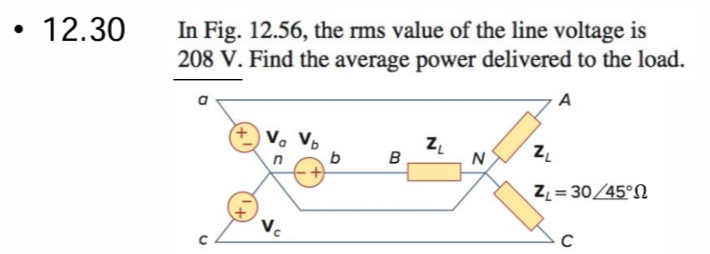
\includegraphics[width=0.8\textwidth]{assets/vboefening 3fase.png}
    \caption{Sterconfiguratie met gelijke belastingen.}
    \label{fig:vboefening 3fase.png}
\end{figure}
\FloatBarrier
\begin{oefenblok}
    \textbf{Uitgewerkt voorbeeld: 3-fase sterconfiguratie met gelijke belastingen}

    \[V_l = 208 V\]
    \[V_f = \frac{V_l}{\sqrt{3}} = \frac{208 V}{\sqrt{3}} = 120.1 V\]
    \[I_f = \frac{V_f}{Z_L} = \frac{120.1 V}{30\angle 45^\circ\ \Omega }\]
    rekenmachine in r<theta modus
    \[I_f = 4.0\angle -45^\circ\ \text{A}\]
    \[P = 3 V_f I_f \cos \phi = 3 \cdot 120.1 V \cdot 4.0 A \cdot \cos 45^\circ = 1021.6 W\]
    \[Q = 3 V_f I_f \sin \phi = 3 \cdot 120.1 V \cdot 4.0 A \cdot \sin 45^\circ = 1021.6 VAR\]
    \[S = P + jQ = 1021.6 W + j 1021.6 VAR = 1445.6 VA\]
\end{oefenblok}

\textbf{Opgave 12.80}

Een evenwichtige driefasige bron voorziet drie belastingen van vermogen. De volgende gegevens zijn bekend:
\begin{itemize}
    \item Belasting 1: $6 \text{ kVA}$ bij $0.83$ pf naijlend
    \item Belasting 2: onbekend
    \item Belasting 3: $8 \text{ kW}$ bij $0.7071$ pf voorijlend
    \item Lijnstroom: $84.6 \text{ A (rms)}$
    \item Lijnspanning aan de belastingen: $208 \text{ V (rms)}$
    \item Gecombineerde belasting arbeidsfactor: $0.8$ naijlend
\end{itemize}

\textbf{Gevraagd:} Bepaal de onbekende belasting (Belasting 2).

\begin{oefenblok}[Bepaling van onbekende belasting met behulp van Complex Vermogen]

    We gebruiken het principe van behoud van complex vermogen. In een systeem met meerdere belastingen geldt:

    $$\mathbf{S}_{\text{totaal}} = \mathbf{S}_1 + \mathbf{S}_2 + \mathbf{S}_3$$

    We kunnen dit herschikken om de onbekende belasting te vinden:

    $$\mathbf{S}_2 = \mathbf{S}_{\text{totaal}} - \mathbf{S}_1 - \mathbf{S}_3$$

    \textbf{Gegeven data}:
    \begin{itemize}
        \item Lijnspanning: $V_L = 208 \text{ V}$
        \item Lijnstroom: $I_L = 84.6 \text{ A}$
        \item Totale arbeidsfactor: $pf = 0.8$ (naijlend)
        \item Belasting 1: $S_1 = 6 \text{ kVA}$ bij $pf_1 = 0.83$ (naijlend)
        \item Belasting 3: $P_3 = 8 \text{ kW}$ bij $pf_3 = 0.7071$ (voorijlend)
        \item Belasting 2: ONBEKEND
    \end{itemize}

    \textbf{Stap 1: Bereken totaal complex vermogen ($\mathbf{S}_{\text{totaal}}$)}

    Schijnbaar vermogen:
    $$S_{\text{totaal}} = \sqrt{3} V_L I_L = \sqrt{3} \times 208 \times 84.6 \approx 30.48 \text{ kVA}$$

    Actief vermogen (met $pf = 0.8$):
    $$P_{\text{totaal}} = S_{\text{totaal}} \times pf = 30.48 \times 0.8 = 24.38 \text{ kW}$$

    Reactief vermogen (met $\sin(\theta) = 0.6$, omdat $0.8^2 + 0.6^2 = 1$):
    $$Q_{\text{totaal}} = S_{\text{totaal}} \times \sin(\theta) = 30.48 \times 0.6 = 18.29 \text{ kVAR}$$

    $$\mathbf{S}_{\text{totaal}} = 24.38 + j18.29 \text{ kVA}$$

    \textbf{Stap 2: Bereken complex vermogen van belasting 1 ($\mathbf{S}_1$)}

    Gegeven: $6 \text{ kVA}$ bij $pf_1 = 0.83$ (naijlend)

    Actief vermogen:
    $$P_1 = 6 \times 0.83 = 4.98 \text{ kW}$$

    Voor reactief vermogen vinden we $\sin(\theta_1)$:
    $$\theta_1 = \cos^{-1}(0.83) \Rightarrow \sin(\theta_1) \approx 0.5578$$
    $$Q_1 = 6 \times 0.5578 = 3.35 \text{ kVAR}$$

    (Positief omdat het naijlend is)

    $$\mathbf{S}_1 = 4.98 + j3.35 \text{ kVA}$$

    \textbf{Stap 3: Bereken complex vermogen van belasting 3 ($\mathbf{S}_3$)}

    Gegeven: $8 \text{ kW}$ bij $pf_3 = 0.7071 = \frac{1}{\sqrt{2}}$ (voorijlend)

    Actief vermogen:
    $$P_3 = 8 \text{ kW}$$

    De arbeidsfactor $0.7071$ komt overeen met $45^\circ$, dus $\tan(45^\circ) = 1$:
    $$Q_3 = P_3 \times \tan(45^\circ) = 8 \times 1 = 8 \text{ kVAR}$$

    \textbf{Let op}: Omdat de arbeidsfactor voorijlend is, is het reactieve vermogen negatief.

    $$\mathbf{S}_3 = 8.0 - j8.0 \text{ kVA}$$

    \textbf{Stap 4: Los op voor onbekende belasting 2 ($\mathbf{S}_2$)}

    Trek de bekende belastingen af van het totale vermogen:

    $$\mathbf{S}_2 = (P_{\text{totaal}} + jQ_{\text{totaal}}) - (P_1 + jQ_1) - (P_3 - jQ_3)$$

    Reëel deel ($P_2$):
    $$P_2 = 24.38 - 4.98 - 8.0 = 11.4 \text{ kW}$$

    Imaginair deel ($Q_2$):
    $$Q_2 = 18.29 - 3.35 - (-8.0) = 18.29 - 3.35 + 8.0 = 22.94 \text{ kVAR}$$

    $$\mathbf{S}_2 = 11.4 + j22.94 \text{ kVA}$$

    \textbf{Stap 5: Bepaal schijnbaar vermogen en arbeidsfactor}

    Schijnbaar vermogen ($S_2$):
    $$S_2 = \sqrt{P_2^2 + Q_2^2} = \sqrt{11.4^2 + 22.94^2} \approx 25.6 \text{ kVA}$$

    Arbeidsfactor ($pf_2$):
    $$pf_2 = \frac{P_2}{S_2} = \frac{11.4}{25.6} \approx 0.445$$

    Omdat het reactieve vermogen ($Q_2$) positief is, is de arbeidsfactor naijlend.

    \textbf{Eindantwoord}

    \textbf{Onbekende belasting 2:}
    \begin{itemize}
        \item Actief vermogen: $P_2 = 11.4 \text{ kW}$
        \item Reactief vermogen: $Q_2 = 22.94 \text{ kVAR}$
        \item Schijnbaar vermogen: $S_2 = 25.6 \text{ kVA}$
        \item Arbeidsfactor: $0.445$ (naijlend)
    \end{itemize}
\end{oefenblok}

\section{Hoofdstuk 5: Elektrische veiligheid}

\begin{examenbox}[EXAMENTIP: dit hoofdstuk zijn gratis punten]
    Veiligheid komt \textbf{gegarandeerd} op het examen: er staat telkens minstens één theorievraag
    over de 5 vitale veiligheidsregels, de MCB-karakteristiek, de werking van de RCD
    (somstroomtransformator), overbelasting versus kortsluiting, of aanraakspanning. Er valt niets
    te rekenen en niets af te leiden --- je kent het of je kent het niet. Dit is dus het goedkoopste
    stuk van de leerstof: een avond studeren staat gelijk aan een zekere score.

    Bovendien is het geen weggegooide moeite. Dezelfde stof komt terug in \textbf{OIS} (Ontwerp van
    een Industriële Sturing) en in \textbf{Distributie van elektrische energie}. Wat je hier leert,
    hoef je daar niet opnieuw te leren.

    De opbouw is:
    \textbf{Gevaren} $\rightarrow$ \textbf{Veilig werken} $\rightarrow$ \textbf{Beveiliging tegen overstroom} $\rightarrow$ \textbf{Bescherming tegen elektrische schokken}.
\end{examenbox}

\subsection{Elektrische gevaren}

Elektriciteit brengt twee fundamentele gevaren met zich mee: risico's voor \textbf{installaties}
(brand, smelten, mechanische vernieling) én voor \textbf{mensen} (elektrocutie, brandwonden, vallen).
Beide categorieën vereisen een specifieke beveiligingstechniek.

\subsubsection{Gevaren voor installaties}

\textbf{Thermische gevaren ($I^2R$).} Elke geleider en contactovergang heeft een ohmse weerstand.
Bij stroomdoorgang wordt elektrisch vermogen omgezet in warmte:
\[P_{\text{verlies}} = I^2 R\]
Bij langdurige overbelasting of een slecht contact stapelt de warmte zich op. Dit tast de
kabelisolatie aan (verbrokkeling, doorslag) en kan leiden tot isolatiebrand. Daarom moeten kabels
correct gedimensioneerd worden volgens de toelaatbare stroomsterkte ($I_z$).

\textbf{Elektrodynamische gevaren (mechanische krachten).} Rond elke stroomvoerende geleider ontstaat
een magnetisch veld. Bij twee evenwijdige geleiders op afstand $d$ oefenen deze velden volgens de
Lorentzkracht een mechanische kracht op elkaar uit:
\[F \sim \frac{\mu_0 \cdot i_1(t) \cdot i_2(t)}{2\pi d}\]
\begin{figure}[H]
    \centering
    \begin{tikzpicture}[x=1cm, y=1cm, >=latex]
        % twee geleiders in doorsnede
        \foreach \x/\lbl/\dir in {0/$i_1$/1, 3.4/$i_2$/1} {
            \draw[fill=schoolOrange!25, draw=schoolOrange!80!black, line width=1pt] (\x,0) circle (0.32);
            \fill[schoolOrange!80!black] (\x,0) circle (0.07);
            \node[font=\small, below=6mm] at (\x,0) {\lbl};
        }
        % veldlijnen
        \foreach \r in {0.62, 0.95, 1.30} {
            \draw[schoolBlue!60, thin] (0,0) circle (\r);
            \draw[schoolBlue!60, thin] (3.4,0) circle (\r);
        }
        \node[font=\scriptsize, schoolBlue!70!black] at (-1.15,1.25) {magnetisch veld};
        % afstand d
        \draw[<->, thick] (0,-1.15) -- (3.4,-1.15) node[midway, below, font=\small] {afstand $d$};
        % krachten (gelijke richting -> aantrekking)
        \draw[->, ultra thick, schoolRed] (0.45,0) -- (1.35,0);
        \draw[->, ultra thick, schoolRed] (2.95,0) -- (2.05,0);
        \node[font=\small, schoolRed, above] at (1.7,0.18) {$F$};
        % toelichting
        \node[font=\scriptsize, anchor=north, align=center] at (1.7,-1.75)
             {stroom in \emph{dezelfde} richting $\rightarrow$ de geleiders trekken elkaar aan\\
              stroom in \emph{tegengestelde} richting $\rightarrow$ ze stoten elkaar af};
    \end{tikzpicture}
    \caption{Twee evenwijdige geleiders in doorsnede. Elke stroom maakt een magnetisch veld, en dat
        veld oefent een kracht uit op de \emph{andere} geleider. De kracht schaalt met het product
        $i_1 i_2$ en dus met het \textbf{kwadraat} van de stroom --- daarom is ze bij normale
        bedrijfsstroom verwaarloosbaar, maar bij een kortsluitpiek van tientallen kiloampères groot
        genoeg om railkokers uit hun steunen te rukken.}
    \label{fig:elektrodynamische-kracht}
\end{figure}
\FloatBarrier

Bij een zware kortsluitstroom (die tot tientallen kiloampères kan pieken) wordt deze kracht
\textbf{evenredig met het kwadraat van de piekstroom ($i_{\text{piek}}^2$)}. Hierdoor kunnen
geleiders en railkokers met enorme kracht naar elkaar toe getrokken of uit elkaar geslagen worden,
wat kasten openscheurt of isolatiesteunen verbrijzelt.

\begin{examenbox}[EXAMENVRAAG:]
    \textit{Waarom is een \textbf{robuuste mechanische verankering} van railkokers en dikke
        vermogenskabels zo cruciaal?}

    Om de enorme \textbf{elektrodynamische krachten} bij kortsluiting op te vangen. De krachten
    schalen met $I_{\text{kortsluit}}^2$; zonder stevige steunen worden geleiders losgerukt, met
    secundaire kortsluitingen en zware schade tot gevolg.
\end{examenbox}

\subsubsection{Directe gevaren voor mensen (elektrische schok)}

Wanneer een menselijk lichaam deel uitmaakt van een gesloten elektrische kring, vloeit er een
lichaamsstroom $I_B$. De directe fysiologische gevolgen zijn:

\begin{itemize}
    \item \textbf{Zenuwstelsel en spieren:} externe elektrische signalen verstoren de neuromusculaire
          sturing. Dit veroorzaakt onwillekeurige contractie van spieren. Bij de \emph{loslaatdrempel}
          ($\approx 10-15\text{ mA}$) kan het slachtoffer de geleider fysiek niet meer loslaten.
          Bij doorgang door de borstkas treedt ademhalingsverlamming op.
    \item \textbf{Hart: ventrikelfibrillatie.} Stroomdoorgang door de hartspier tijdens de kwetsbare
          T-fase van de hartcyclus verstoort het synchrone samentrekken. Het hart gaat chaotisch
          trillen ($>400\text{ slagen/min}$) en pompt geen bloed meer rond. Zonder defibrillatie
          treedt binnen enkele minuten hersendood op.
    \item \textbf{Brandwonden:} joule-opwarming ($I_B^2 R_{\text{weefsel}} t$) veroorzaakt ernstige
          uitwendige én inwendige weefselverbranding. Inwendige brandwonden zijn levensbedreigend
          omdat ze pas uren later tot necrose en orgaanfalen leiden.
    \item \textbf{Elektrolyse en ionisatie:} bij gelijkstroom en langdurige AC worden vloeistoffen
          en celmembranen chemisch ontleed.
\end{itemize}

De ernst van het letsel wordt bepaald door \textbf{zes sleutelfactoren}:
\begin{enumerate}
    \item \textbf{Stroomsterkte $I_B$} --- hoe groter de stroom, hoe zwaarder het effect.
    \item \textbf{Lichaamsimpedantie $Z_B$} --- bepaalt bij een gegeven spanning de stroom
          ($I_B = V/Z_B$). Droge eeltlaag heeft een hoge weerstand ($>2000\,\Omega$), natte of
          beschadigde huid zakt naar $<500-1000\,\Omega$.
    \item \textbf{Frequentie $f$} --- netfrequentie ($50-60\text{ Hz}$) is fysiologisch het
          gevaarlijkst omdat dit nauw aansluit bij de resonantiefrequentie van het menselijk
          zenuwstelsel. Bij hoge frequenties ($>10\text{ kHz}$) treedt minder spierprikkeling op
          (vooral warmte-effect).
    \item \textbf{Blootstellingsduur $t$} --- hoe langer de stroom vloeit, hoe groter de kans dat
          de kwetsbare hartfase geraakt wordt en hoe meer warmte gedissipeerd wordt.
    \item \textbf{Aanraakspanning $V$} --- drijft de stroom door het lichaam en doorbreekt bij
          hogere waarden de huidbarrière.
    \item \textbf{Stroombaan door het lichaam} --- trajecten over het hart (bv.\ linkerhand naar
          voeten, hand naar hand) zijn veel risicovoller dan van voet naar voet.
\end{enumerate}

\begin{waarschuwing}[Niet de spanning maar de stroom doodt!]
    De fysiologische schade hangt direct af van de \textbf{stroom $I_B$} door het lichaam en de
    tijdsduur $t$. Omdat $I_B = V_{\text{aanraak}}/Z_B$, zijn internationale veiligheidsnormen
    primair opgesteld in milliampères (mA) en pas secundair omgerekend naar spanningen (V).
\end{waarschuwing}

\subsubsection{De AC-zonegrafiek (IEC 60479) en de uitschakelkromme}

De norm IEC 60479 beschrijft de fysiologische effecten van wisselstroom ($50/60\text{ Hz}$) in
functie van stroomsterkte $I_B$ en tijdsduur $t$.

\begin{figure}[htbp]
    \centering
    \begin{tikzpicture}[scale=0.95]
        % assen
        \draw[->, thick] (0,0) -- (11,0) node[right] {$I_B$ [mA]};
        \draw[->, thick] (0,0) -- (0,6.4) node[above] {$t$ [ms]};
        % x-ticks
        \foreach \x/\l in {0.6/0.5, 2.4/5, 4.6/50, 6.4/500, 8.6/2000, 10.2/10000}
        \draw (\x,0) -- (\x,-0.12) node[below, font=\scriptsize] {\l};
        % y-ticks
        \foreach \y/\l in {0.8/10, 2.0/100, 3.4/1000, 5.2/10000}
        \draw (0,\y) -- (-0.12,\y) node[left, font=\scriptsize] {\l};
        % zone-grenzen
        \draw[thick, dashed] (0.6,0) -- (0.6,6.0);
        \draw[thick, dashed] (2.4,6.0) -- (2.4,3.0) -- (4.6,0);
        \draw[thick, schoolRed] (5.0,6.0) -- (5.0,3.2) .. controls (5.6,2.4) .. (6.4,1.6) -- (6.4,0);
        \draw[thick, schoolRed, dash pattern=on 3pt off 2pt]
        (7.2,6.0) -- (7.2,3.0) .. controls (7.6,2.2) .. (8.2,1.4) -- (8.2,0);
        \draw[thick, schoolRed, dash pattern=on 1pt off 2pt]
        (8.9,6.0) -- (8.9,2.8) .. controls (9.3,2.0) .. (9.9,1.2) -- (9.9,0);
        % zonelabels
        \node[font=\small\bfseries, schoolGreen] at (0.3,3.2) {\rotatebox{90}{AC-1}};
        \node[font=\small\bfseries, schoolGreen] at (1.5,3.2) {AC-2};
        \node[font=\small\bfseries, schoolOrange] at (3.6,3.6) {AC-3};
        \node[font=\small\bfseries, schoolRed] at (8.6,4.6) {AC-4};
        % curvelabels
        \node[font=\scriptsize] at (0.6,6.25) {a};
        \node[font=\scriptsize] at (2.4,6.25) {b};
        \node[font=\scriptsize, schoolRed] at (5.0,6.25) {$c_1$};
        \node[font=\scriptsize, schoolRed] at (7.2,6.25) {$c_2$};
        \node[font=\scriptsize, schoolRed] at (8.9,6.25) {$c_3$};
        % AC-4 onderverdeling
        \node[font=\tiny, schoolRed] at (6.1,4.6) {\rotatebox{90}{AC-4.1}};
        \node[font=\tiny, schoolRed] at (7.9,4.6) {\rotatebox{90}{AC-4.2}};
        \node[font=\tiny, schoolRed] at (9.6,4.6) {\rotatebox{90}{AC-4.3}};
    \end{tikzpicture}
    \caption{Effect van wisselstroom op het menselijk lichaam volgens IEC 60479 (logaritmische assen).}
    \label{fig:ac-zones}
\end{figure}
\FloatBarrier

\begin{itemize}
    \item \textbf{Zone AC-1 ($I_B < 0{,}5\text{ mA}$):} onder de waarnemingsdrempel (curve a). Geen merkbaar effect.
    \item \textbf{Zone AC-2 ($0{,}5\text{ mA} \le I_B \le \text{curve b}$):} waarneembaar, lichte spiertinteling,
          maar geen schadelijke fysiologische gevolgen.
    \item \textbf{Zone AC-3 (curve b tot $c_1$):} spierverkramping, ademhalingsmoeilijkheden, loslaten niet meer
          mogelijk. Effecten zijn \emph{omkeerbaar} zodra de stroom onderbroken wordt.
    \item \textbf{Zone AC-4 (boven curve $c_1$):} levensgevaar door \belangrijk{ventrikelfibrillatie}, hartstilstand
          en ernstige brandwonden:
          \begin{itemize}
              \item AC-4.1: kans op ventrikelfibrillatie tot $5\%$ (curve $c_1$ tot $c_2$).
              \item AC-4.2: kans op ventrikelfibrillatie tot $50\%$ (curve $c_2$ tot $c_3$).
              \item AC-4.3: kans op ventrikelfibrillatie $>50\%$ (boven curve $c_3$).
          \end{itemize}
\end{itemize}

\begin{figure}[htbp]
    \centering
    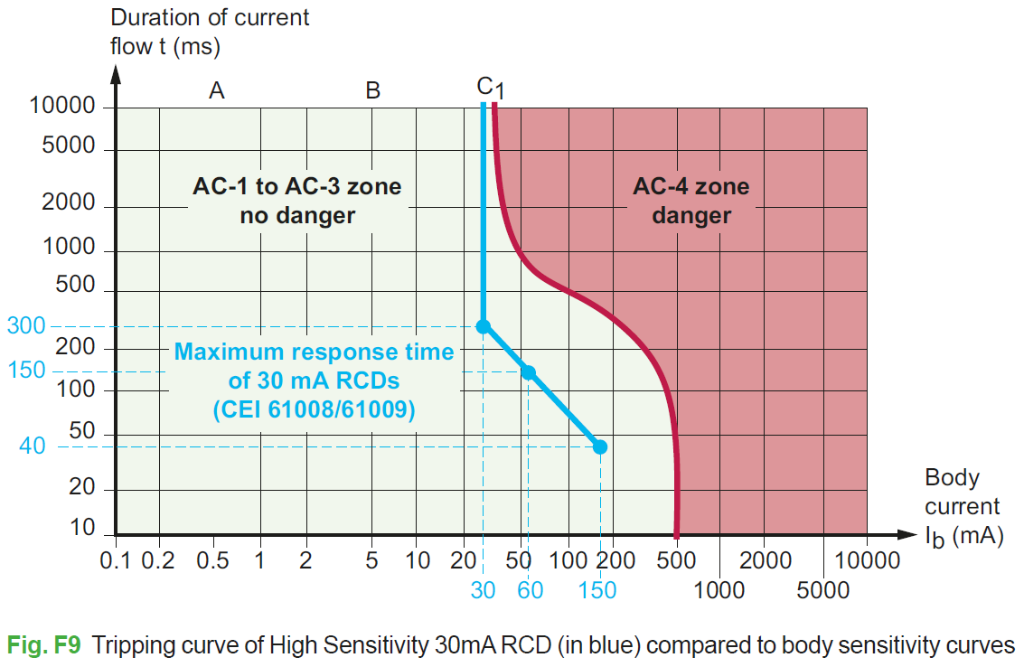
\includegraphics[width=0.75\textwidth]{assets/rcd_tripping_curve.png}
    \caption{Uitschakelkarakteristiek van een hooggewelige $30\text{ mA}$ aardlekschakelaar (in blauw)
        geprojecteerd op de IEC 60479 gevarenzones. De automaat schakelt altijd uit vóór curve $c_1$
        (gevarenzone AC-4) bereikt wordt.}
    \label{fig:rcd-tripping-curve}
\end{figure}
\FloatBarrier

\begin{examenbox}[EXAMENVRAAG:]
    \textit{Benoem de assen van deze grafiek en verklaar waarom de grenzen schuin verlopen.}

    \textbf{Assen:} Horizontaal de \textbf{lichaamsstroom $I_B$} in mA (logaritmisch), verticaal de
    \textbf{duur $t$} in ms (logaritmisch).

    \textbf{Vorm:} De grenslijnen buigen schuin naar beneden omdat een grotere stroom slechts gedurende
    een veel kortere tijd getolereerd kan worden vóór fibrillatie optreedt. Bij zeer korte tijden
    ($<10-30\text{ ms}$) is het gevaar drastisch lager omdat de kans klein is dat de stroom exact in de
    kwetsbare T-golf van de hartslag valt. \textbf{Precies daarom biedt een snelle RCD ($<30\text{ ms}$)
        optimale persoonsbescherming.}
\end{examenbox}

\subsubsection{Van stroom naar aanraakspanning (BB-condities)}

Omdat men in een installatie enkel de spanning kan beheersen, wordt via de conventionele
lichaamsweerstand $Z_B$ de stroomgrens omgerekend naar een \textbf{veilige conventionele aanraakspanningsgrens} ($U_L$):
\[I_B = \frac{U_{\text{aanraak}}}{Z_B}\]

\begin{center}
    \begin{tabular}{@{}llcc@{}}
        \toprule
        \textbf{Code} & \textbf{Omgevingsconditie}                   & \textbf{Grens AC ($U_L$)} & \textbf{Grens DC ($U_L$)} \\
        \midrule
        \textbf{BB1}  & Droge omgeving (normale huid, droge vloer)   & $50\text{ V}$             & $120\text{ V}$            \\
        \textbf{BB2}  & Vochtige omgeving (natte huid, natte voeten) & $25\text{ V}$             & $60\text{ V}$             \\
        \textbf{BB3}  & Ondergedompeld (zwembad, badkuip)            & $12\text{ V}$             & $30\text{ V}$             \\
        \bottomrule
    \end{tabular}
\end{center}

\begin{figure}[htbp]
    \centering
    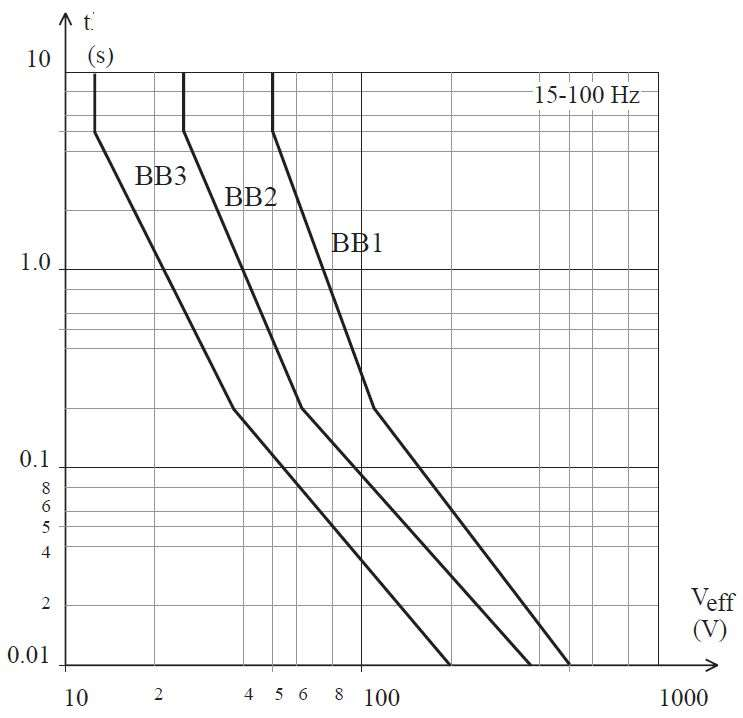
\includegraphics[width=0.65\textwidth]{assets/touch_voltage_curves_bb.png}
    \caption{Maximale uitschakeltijd $t$ in functie van de effectieve aanraakspanning $V_{\text{eff}}$
        voor condities BB1, BB2 en BB3. Links van de knik ($50\text{ V}$ bij BB1, $25\text{ V}$ bij BB2,
        $12\text{ V}$ bij BB3) mag de spanning oneindig lang blijven bestaan.}
    \label{fig:touch-voltage-curves}
\end{figure}
\FloatBarrier

\subsubsection{Rechtstreekse versus onrechtstreekse aanraking}

\begin{itemize}
    \item \textbf{Rechtstreekse aanraking (Direct contact):} een persoon raakt een actieve geleider aan die
          in normale toestand onder spanning staat (bv.\ fasedraad L1).
          \emph{Beveiliging:} isolatie, omhulsels/kasten (IP-graad), afstand/afscherming, en als
          bijkomende bescherming een $30\text{ mA}$ RCD.
    \item \textbf{Onrechtstreekse aanraking (Indirect contact):} een persoon raakt een metalen
          geleidend gestel aan dat \emph{normaal spanningsloos} is, maar door een intern defect
          (isolatiefout) onder spanning is komen te staan.
          \emph{Beveiliging:} aarding van alle gestellen via beschermingsgeleider (PE) gekoppeld aan
          een automatische uitschakeling (RCD of overstroombeveiliging).
\end{itemize}

Figuur~\ref{fig:indirect-contact-slide} toont het geval dat op het examen telkens terugkomt: een
isolatiefout zet het metalen gestel onder spanning, de foutstroom $I_{\text{fault}}$ zoekt zijn weg
via de beschermingsgeleider (PE) naar de aarde, en tussen het gestel en de grond staat de
aanraakspanning $U_z$. Figuur~\ref{fig:indirect-contact-tikz} zet daar het elektrische
vervangingsschema naast, met de weerstanden die je nodig hebt om $U_z$ te berekenen.

\begin{figure}[htbp]
    \centering
    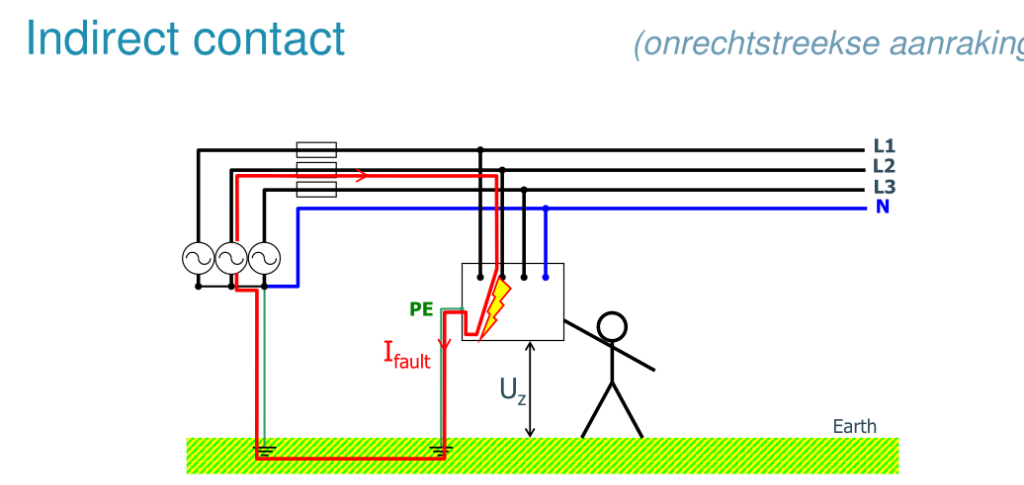
\includegraphics[width=0.88\textwidth]{assets/indirect_contact.png}
    \caption{Onrechtstreekse aanraking: door een isolatiefout staat het gestel onder spanning. De
        foutstroom $I_{\text{fault}}$ loopt via PE naar de aarde; $U_z$ is de aanraakspanning.}
    \label{fig:indirect-contact-slide}
\end{figure}
\FloatBarrier

\begin{figure}[htbp]
    \centering
    \begin{circuitikz}[scale=0.92, transform shape]
        % bron
        \draw (0,0) to[sV={$U_0 = 230$~V}, i<^=$I_f$] (0,3.4);
        % isolatiefout naar het gestel
        \draw (0,3.4) to[R, l_={$R_f$}] (3.2,3.4);
        \node[font=\scriptsize, schoolRed, above] at (1.6,3.72) {isolatiefout};
        \draw (3.2,3.4) -- (6.4,3.4) node[circ]{};
        \node[font=\scriptsize, above, align=center] at (4.8,3.55) {metalen gestel};
        % aardverspreidingsweerstand van de gebruiker
        \draw (6.4,3.4) to[R={$R_A$}] (6.4,0);
        % de persoon
        \draw (6.4,3.4) -- (9.0,3.4) to[R={$R_B$}] (9.0,0) node[circ]{};
        \node[font=\scriptsize, above, align=center] at (9.0,3.55) {persoon};
        % transformatoraarding in de terugweg
        \draw (0,0) to[R={$R_N$}] (3.2,0);
        \draw (3.2,0) -- (9.0,0);
        \node[font=\scriptsize, below] at (5.0,-0.15) {aarde};
        % aanraakspanning
        \draw[<->, thick, schoolBlue] (10.4,3.4) -- (10.4,0);
        \node[font=\footnotesize, schoolBlue, right, align=left] at (10.5,1.7)
             {$U_T = I_f\cdot R_A$\\\scriptsize aanraakspanning};
        \draw[dashed, gray!70] (9.0,3.4) -- (10.4,3.4);
        \draw[dashed, gray!70] (9.0,0) -- (10.4,0);
        \draw (0,0) node[ground]{};
    \end{circuitikz}
    \caption{Vervangingsschema van onrechtstreekse aanraking in een TT-net. De foutstroom $I_f$ loopt
        via het gestel en $R_A$ terug naar de transformatoraarding $R_N$; over $R_A$ staat de
        aanraakspanning $U_T$. De persoon ($R_B \approx 1000\,\Omega$) staat parallel met $R_A$
        ($30\,\Omega$) en verandert de foutstroom dus nauwelijks --- daarom laat je $R_B$ weg bij het
        berekenen van $I_f$, en gebruik je hem pas achteraf om $I_B = U_T/R_B$ te vinden.}
    \label{fig:indirect-contact-tikz}
\end{figure}
\FloatBarrier

\frm{Foutstroom bij indirect contact (TT-net)}{I_f = \frac{U_0}{R_A + R_N + R_f}}
{Met $U_0$ de fasespanning ($230\text{ V}$), $R_A$ de aardverspreidingsweerstand van de gebruiker in $\Omega$, $R_N$ de transformatoraarding in $\Omega$ en $R_f$ de foutweerstand in $\Omega$.}

\frm{Aanraakspanning (foutspanning)}{U_T = I_f \cdot R_A = U_0 \cdot \frac{R_A}{R_A + R_N + R_f}}
{Met $U_T$ de spanning tussen het defecte gestel en de referentie-aarde in V.}

\frm{Veiligheidsvoorwaarde in TT-netten}{R_A \cdot I_{\Delta n} \le U_L \qquad \Longleftrightarrow \qquad R_A \le \frac{U_L}{I_{\Delta n}}}
{Met $I_{\Delta n}$ de nominale aanspreekstroom van de RCD (bv.\ $30\text{ mA}$ of $300\text{ mA}$) en $U_L$ de conventionele grensaanraakspanning ($50\text{ V}$ voor BB1, $25\text{ V}$ voor BB2).}

\begin{oefening}[Waarom een MCB niet volstaat en een RCD strikt noodzakelijk is]
    \textbf{Gegeven (TT-netwerk):} $U_0 = 230\text{ V}$, transformatoraarding $R_N = 10\,\Omega$, aardverspreidingsweerstand $R_A = 30\,\Omega$, isolatiefout $R_f = 0\,\Omega$, kring beveiligd met een MCB $16\text{ A}$ (type C) en een RCD $30\text{ mA}$. Lichaamsweerstand $R_B = 1000\,\Omega$.

    \textbf{Berekening:}
    \begin{enumerate}
        \item \textbf{Foutstroom door de aarding:}
              \[I_f = \frac{230\text{ V}}{30\,\Omega + 10\,\Omega} = \mathbf{5{,}75\text{ A}}\]
        \item \textbf{Aanraakspanning op het toestel:}
              \[U_T = I_f \cdot R_A = 5{,}75\text{ A} \cdot 30\,\Omega = \mathbf{172{,}5\text{ V}} \qquad (\gg 50\text{ V} \text{ levensgevaarlijk!})\]
        \item \textbf{Lichaamsstroom bij aanraking:}
              \[I_B = \frac{U_T}{R_B} = \frac{172{,}5\text{ V}}{1000\,\Omega} = \mathbf{172{,}5\text{ mA}} \qquad (\text{Zone AC-4: dodelijk binnen } <0{,}5\text{ s})\]
        \item \textbf{Reactie van de MCB ($16\text{ A}$ type C):}
              Een automaat van $16\text{ A}$ type C heeft een magnetische drempel van $5 \times 16\text{ A} = \mathbf{80\text{ A}}$. Bij een foutstroom van $5{,}75\text{ A}$ reageert de MCB \belangrijk{nooit}!
        \item \textbf{Reactie van de RCD ($30\text{ mA}$):}
              Omdat $I_f = 5{,}75\text{ A} \gg 30\text{ mA}$, schakelt de RCD \textbf{onmiddellijk uit} ($<30\text{ ms}$), waardoor de spanning wegvalt vóór ventrikelfibrillatie kan optreden.
    \end{enumerate}
\end{oefening}

\subsubsection{Secundaire en indirecte gevaren}

\textbf{Secundaire letsels (vallen/schrikreactie).} De spierreflex na een lichte schok kan leiden tot
vallen van een ladder of contact met draaiende machines. Bij redding: raak het slachtoffer nooit met
blote handen aan zolang de spanning niet is afgeschakeld; gebruik droog isolerend materiaal.

\textbf{De elektrische vlamboog (Arc Flash).} Bij kortsluiting ioniseert de lucht en ontstaat een
plasma van duizenden graden Celsius. De vier gevaren:
\begin{enumerate}
    \item \textbf{Extreem thermisch geweld:} smelten en wegspatten van gloeiend vloeibaar koper.
    \item \textbf{Giftige gassen:} verdampend koper oxideert tot zware toxische rookgassen.
    \item \textbf{Intens UV- en infraroodlicht:} veroorzaakt acute netvliesverbranding (lasogen) en huidverbranding.
    \item \textbf{Akoestische drukgolf (Arc Blast):} plotse luchtuitzetting met knal ($>140\text{ dB}$) die
          trommelvliezen scheurt en personen wegslingert.
\end{enumerate}

\subsection{Veilig werken met elektriciteit}

\subsubsection{De vijf gouden veiligheidsregels}

Bij werkzaamheden aan elektrische installaties moeten de \textbf{vijf procedurestappen} in
\textbf{strikte volgorde} worden toegepast:

\begin{figure}[htbp]
    \centering
    \begin{tikzpicture}[
        node distance=0mm,
        stap/.style={draw=schoolBlue!70, fill=schoolBlue!6, line width=0.8pt, rounded corners=2.5pt,
                     text width=30mm, align=center, inner sep=2.2mm, font=\footnotesize},
        nr/.style={circle, fill=schoolBlue, text=white, font=\scriptsize\bfseries, inner sep=1.3pt},
        pijl/.style={-{Latex[length=2.4mm]}, line width=1.1pt, schoolBlue!80}
      ]
      \node[stap] (s1) at (0,0) {\textbf{Vrijschakelen}\\[0.5mm]\scriptsize\emph{cut-off}};
      \node[stap] (s2) at (3.6,0) {\textbf{Vergrendelen}\\[0.5mm]\scriptsize\emph{lockout}};
      \node[stap] (s3) at (7.2,0) {\textbf{Meten}\\[0.5mm]\scriptsize\emph{verify}};
      \node[stap] (s4) at (10.8,0) {\textbf{Aarden en kortsluiten}\\[0.5mm]\scriptsize\emph{earth}};
      \node[stap] (s5) at (14.4,0) {\textbf{Afbakenen}\\[0.5mm]\scriptsize\emph{delineate}};

      \foreach \a/\b in {s1/s2, s2/s3, s3/s4, s4/s5}
        \draw[pijl] (\a) -- (\b);

      \foreach \n/\lbl in {s1/1, s2/2, s3/3, s4/4, s5/5}
        \node[nr] at ([shift={(-13.5mm,5.2mm)}]\n.north) {\lbl};

      \node[font=\scriptsize\itshape, schoolRed, align=center] at (7.2,-2.0)
           {strikte volgorde --- een stap overslaan maakt alle volgende stappen waardeloos};
    \end{tikzpicture}
    \caption{De vijf gouden regels voor werken aan een elektrische installatie, in de volgorde
        waarin je ze moet uitvoeren.}
    \label{fig:vijf-gouden-regels}
\end{figure}
\FloatBarrier

\begin{figure}[htbp]
    \centering
    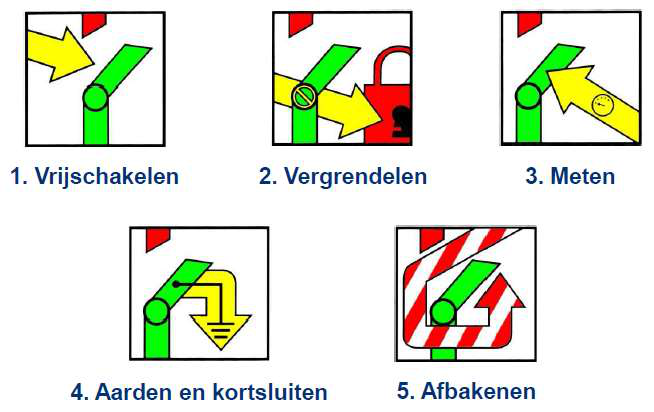
\includegraphics[width=0.62\textwidth]{assets/veilige_vijf_slide.png}
    \caption{Dezelfde vijf stappen zoals ze in de cursus staan (``de Veilige Vijf''). Leer deze
        vijf woorden uit het hoofd --- de vraag op het examen is letterlijk ``geef de vijf gouden
        regels''.}
    \label{fig:veilige-vijf-slide}
\end{figure}
\FloatBarrier

\begin{enumerate}
    \item \textbf{Vrijschakelen.} Alle polen \'en alle mogelijke voedingsbronnen
          scheiden, dus ook noodstroomaggregaten, PV-omvormers en condensatorbatterijen. Een
          condensatorbatterij staat nog onder spanning nadat je de hoofdschakelaar hebt omgelegd.
    \item \textbf{Vergrendelen.} Schakelaars mechanisch vergrendelen met een
          hangslot en een waarschuwingslabel erop. Iemand anders mag jouw kring niet kunnen
          inschakelen terwijl jij eraan werkt.
    \item \textbf{Meten.} Controleer de spanningsloosheid met een goedgekeurde tweepolige
          spanningsaanwijzer, en \belangrijk{het meettoestel testen op een gekende spanningsbron vlak
          v\'o\'or \'en vlak na de meting}. Een stuk meetsnoer dat onderweg breekt geeft anders precies
          hetzelfde beeld als een spanningsloze installatie.
    \item \textbf{Aarden en kortsluiten.} De geleiders onderling en met de aarde verbinden. Verplicht
          bij hoogspanning, aanbevolen bij laagspanning, om inductieve en capacitieve restspanningen
          af te voeren.
    \item \textbf{Afbakenen.} Nabijgelegen delen die nog onder spanning staan fysiek
          afschermen met isolerende doeken of schotten, en de werkzone markeren.
\end{enumerate}

\subsubsection{Regelgeving, keurmerken en uitwendige invloeden}

\begin{itemize}
    \item \textbf{Europese Laagspanningsrichtlijn (LVD 2014/35/EU):} legt fundamentele veiligheidseisen
          op voor elektrisch materiaal tussen $50-1000\text{ V}$ AC en $75-1500\text{ V}$ DC.
    \item \textbf{AREI (Algemeen Reglement op de Elektrische Installaties):} het bindende Belgische
          wetboek voor veilige installaties.
    \item \textbf{Norminstituten:} \textbf{IEC} (mondiaal), \textbf{CENELEC} (Europees) en \textbf{CEBEC/NBN} (België).
\end{itemize}

\begin{figure}[htbp]
    \centering
    \begin{minipage}{0.42\textwidth}
        \centering
        
\includegraphics[width=\textwidth]{assets/keurmerken_certificaten.png}
        \caption{Officiële keurmerken (CE, CEBEC, VDE, KEMA, IEC, UL).}
        \label{fig:keurmerken}
    \end{minipage}\hfill
    \begin{minipage}{0.54\textwidth}
        \centering
        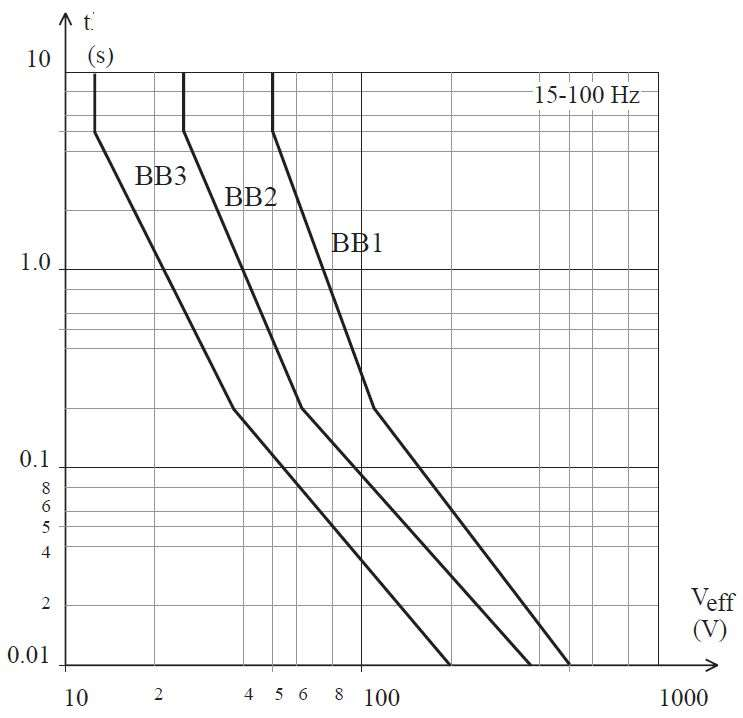
\includegraphics[width=\textwidth]{assets/iec_voltage_ranges.png}
        \caption{IEC spanningsbereiken (AC \& DC).}
        \label{fig:iec-voltage-ranges}
    \end{minipage}
\end{figure}
\FloatBarrier

\textbf{Uitwendige invloeden (AREI-codering):} elektrische apparatuur moet bestand zijn tegen de
omgeving waarin ze geplaatst wordt. Dit wordt aangeduid met een 2-lettercode:
\begin{itemize}
    \item \textbf{Eerste letter (Categorie):}
          \begin{itemize}
              \item \textbf{A} = Milieu/omgeving (bv.\ \textbf{AA}: temperatuur, \textbf{AD}: aanwezigheid van water, \textbf{AE}: stof, \textbf{AG}: mechanische schokken).
              \item \textbf{B} = Personen (bv.\ \textbf{BA}: bekwaamheid van personen --- BA1 gewone mensen, BA4 gewaarschuwd, BA5 bevoegd/vakmensen; \textbf{BB}: lichaamsweerstand/vocht; \textbf{BC}: contact met aardpotentiaal).
              \item \textbf{C} = Gebouwconstructie (bv.\ \textbf{CA}: brandbare bouwmaterialen, \textbf{CB}: evacuatiemogelijkheden/hoogbouw).
          \end{itemize}
    \item \textbf{Cijfer (Klasse):} geeft de graad van zwaarte aan (bv.\ AD1 = droog, AD4 = spatwater, AD7 = onderdompeling).
\end{itemize}

\begin{figure}[htbp]
    \centering
    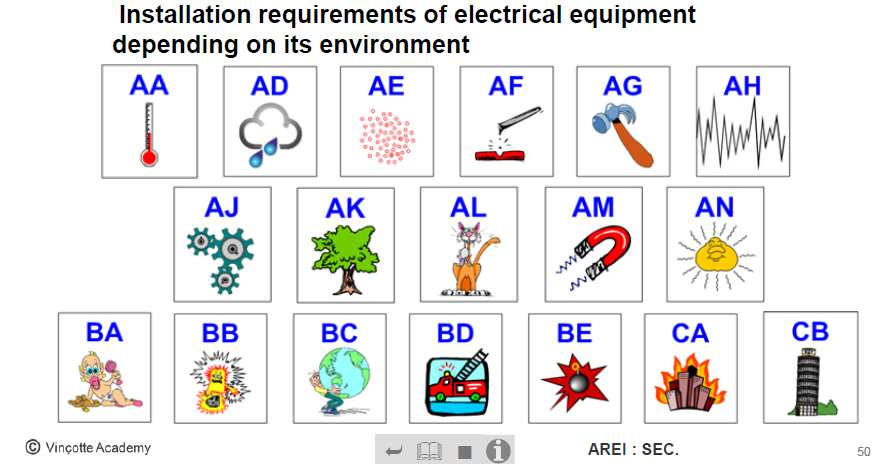
\includegraphics[width=0.85\textwidth]{assets/external_influences.jpeg}
    \caption{Overzicht van de uitwendige invloedscodes volgens AREI / Vinçotte.}
    \label{fig:external-influences}
\end{figure}
\FloatBarrier

\subsubsection{Spanningsklassen volgens IEC}

\begin{center}
    \begin{tabular}{@{}lcc@{}}
        \toprule
        \textbf{Spanningsbereik}                 & \textbf{Wisselspanning (AC)}      & \textbf{Gelijkspanning (DC)} \\
        \midrule
        \textbf{Hoogspanning (HV)}               & $> 1000\text{ V}_{\text{eff}}$    & $> 1500\text{ V}$            \\
        \textbf{Laagspanning (LV)}               & $50 - 1000\text{ V}_{\text{eff}}$ & $120 - 1500\text{ V}$        \\
        \textbf{Zeer lage spanning (ELV / ZLVS)} & $\le 50\text{ V}_{\text{eff}}$    & $\le 120\text{ V}$           \\
        \bottomrule
    \end{tabular}
\end{center}

\subsection{Bescherming tegen overstroom}

\subsubsection{Overbelasting versus kortsluiting}

Een overstroom is elke stroom die hoger is dan de nominale stroom $I_n$ van de kring. We maken een
fundamenteel onderscheid tussen overbelasting en kortsluiting:

\begin{center}
    \begin{tabular}{@{}p{24mm}p{48mm}p{50mm}@{}}
        \toprule
                               & \textbf{Overbelasting (Overload)}                                   & \textbf{Kortsluiting (Short-circuit)}                                        \\
        \midrule
        \textbf{Oorzaak}       & Te veel verbruikers aangesloten of mechanisch geblokkeerde motor.   & Foutieve verbinding met verwaarloosbare impedantie tussen actieve geleiders. \\[1mm]
        \textbf{Stroompad}     & De stroom volgt de \emph{normale geleiders}.                        & De stroom neemt een \emph{abnormaal kort pad}.                               \\[1mm]
        \textbf{Grootte}       & Typisch $1{,}1$ tot $5 \times I_n$.                                 & Tot tientallen of honderden malen $I_n$ ($>10-100 \times I_n$).              \\[1mm]
        \textbf{Gevaar}        & Trage thermische degradatie van de kabelisolatie, brand op termijn. & Explosie, vlamboog, elektrodynamische vernieling van installatiedelen.       \\[1mm]
        \textbf{Detectie}      & \textbf{Thermisch} (bimetaal dat opwarmt).                          & \textbf{Magnetisch} (elektromagnetische spoel).                              \\[1mm]
        \textbf{Uitschakeling} & \textbf{Vertraagd} (invers-tijd: seconden tot minuten).             & \textbf{Quasi ogenblikkelijk} ($<10-20\text{ ms}$).                          \\
        \bottomrule
    \end{tabular}
\end{center}

\begin{figure}[htbp]
    \centering
    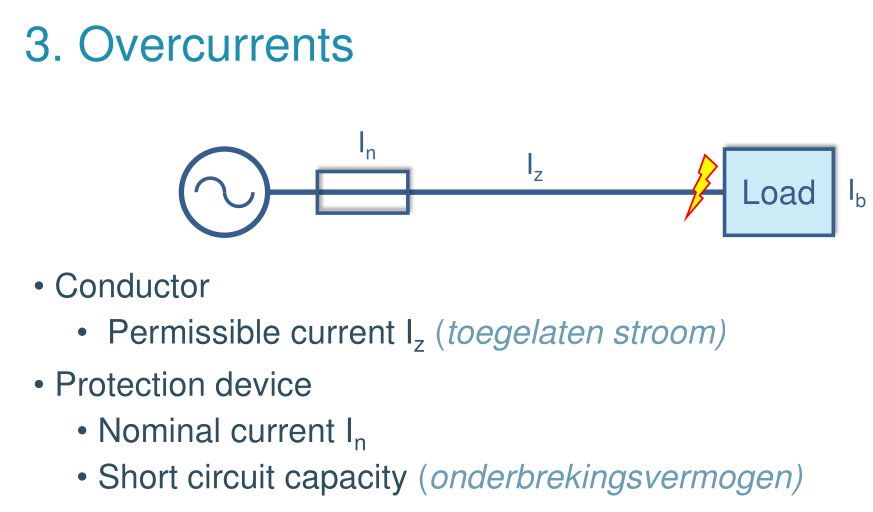
\includegraphics[width=0.72\textwidth]{assets/overcurrents_in_iz_ib.png}
    \caption[Relatie van de ontwerpstromen]{Relatie van de ontwerpstromen voor kabelbeveiliging: $I_b \le I_n \le I_z$.}
    \label{fig:overcurrents}
\end{figure}
\FloatBarrier

\frm{Dimensioneringsregel kabelbeveiliging}{I_b \le I_n \le I_z \qquad\text{en}\qquad I_2 \le 1{,}45 \cdot I_z}
{Met $I_b$ de ontwerpstroom van de belasting, $I_n$ de nominale stroom van de automaat, $I_z$ de toelaatbare continue kabelstroom en $I_2$ de conventionele aanspreekstroom ($1{,}45\,I_n$).}

\frm{Thermische kortsluitvastheid (Adiabatische formule)}{I_{\text{ks}}^2 t \le k^2 S^2 \qquad \Longrightarrow \qquad S_{\text{min}} = \frac{I_{\text{ks}} \sqrt{t}}{k}}
{Met $I_{\text{ks}}$ de kortsluitstroom in A, $t$ de uitschakeltijd van de automaat in s, $S$ de koperdoorsnede in $\text{mm}^2$ en $k$ de materiaalconstante ($k = 115$ voor koper met PVC-isolatie, $k = 143$ voor koper met XLPE-isolatie).}

\begin{theorie}[Stappenplan: Keuze en dimensionering van kabel en automaat]
    \begin{enumerate}
        \item \textbf{Bepaal de bedrijfsstroom $I_b$:} $I_b = \frac{P}{U\cos\phi}$ (1-fase) of $I_b = \frac{P}{\sqrt{3}U\cos\phi}$ (3-fase).
        \item \textbf{Kies de nominale automaatstroom $I_n$:} Neem de eerstvolgende standaardwaarde $I_n \ge I_b$ (bv.\ $16\text{ A}, 20\text{ A}, 25\text{ A}, 32\text{ A}$).
        \item \textbf{Kies de kabeldoorsnede $S$ zodat $I_z \ge I_n$:} volgens de AREI-tabel (bv.\ $1{,}5\text{ mm}^2 \to 16\text{ A}$, $2{,}5\text{ mm}^2 \to 20\text{ A}$, $4\text{ mm}^2 \to 25\text{ A}$, $6\text{ mm}^2 \to 32\text{ A}$).
        \item \textbf{Controleer de kortsluitvastheid:} bereken $S_{\text{min}} = \frac{I_{\text{ks}}\sqrt{t}}{k}$ en controleer dat $S \ge S_{\text{min}}$.
        \item \textbf{Controleer het spanningsverlies $\Delta U$:} $\Delta U = 2 \cdot \frac{\rho \cdot L \cdot I_b}{S}$ (1-fase) en zorg dat $\Delta U \le 3\%$ ($6{,}9\text{ V}$).
    \end{enumerate}
\end{theorie}

\subsubsection{Smeltzekeringen}

De oudste vorm van overstroombeveiliging is de \textbf{smeltzekering}: een dun geleiderdraadje in
een porseleinen of glazen patroon dat doorsmelt zodra $I^2t$ te groot wordt. Ze zijn goedkoop,
uiterst snel bij zware kortsluitstromen en hebben een hoog schakelvermogen. Nadeel is dat je ze na
elke fout moet vervangen, dat er geen thermische en magnetische zone apart instelbaar is, en dat
iemand er een te zware zekering in kan draaien.

\begin{figure}[htbp]
    \centering
    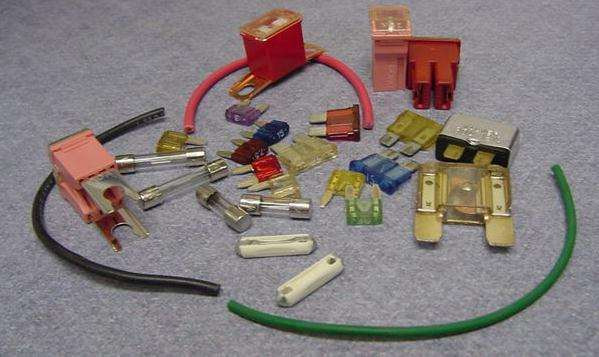
\includegraphics[width=0.55\textwidth]{assets/fuses_smeltzekeringen.png}
    \caption{Smeltzekeringen in verschillende bouwvormen en kalibers.}
    \label{fig:smeltzekeringen}
\end{figure}
\FloatBarrier

In nieuwe installaties zijn ze grotendeels vervangen door de installatieautomaat, die je gewoon
opnieuw kan inschakelen.

\subsubsection{De installatieautomaat (MCB) en zijn uitschakelcurves}

Een \keyterm{MCB (Miniature Circuit Breaker)} combineert een thermische ontgrendeling (bimetaal)
voor overbelasting en een magnetische ontgrendeling (plunjer/spoel) voor kortsluiting.

\begin{figure}[htbp]
    \centering
    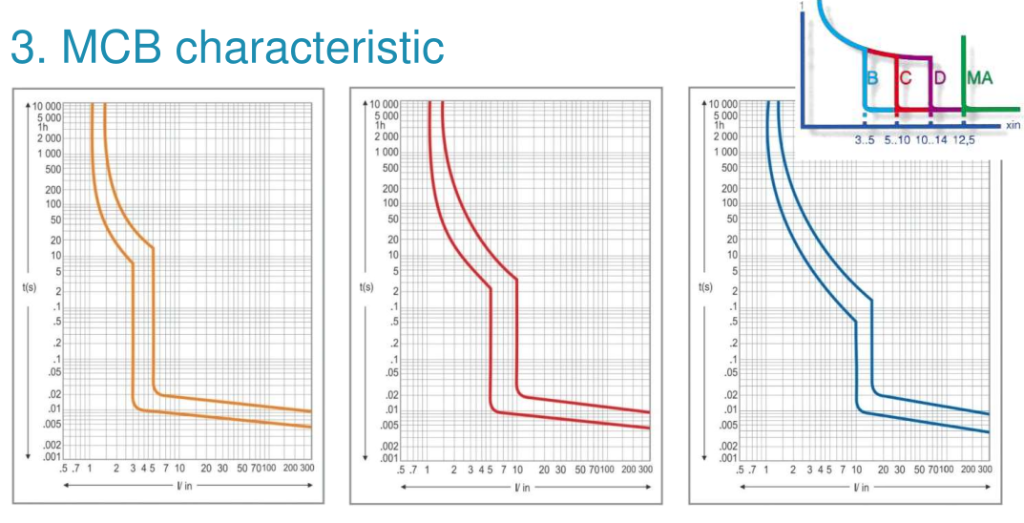
\includegraphics[width=0.95\textwidth]{assets/mcb_karakteristiek_curves.png}
    \caption{Uitschakelkarakteristieken van installatieautomaten volgens IEC 60898 (types B, C, D en MA).}
    \label{fig:mcb-curves-all}
\end{figure}
\FloatBarrier

\begin{examenbox}[EXAMENVRAAG: MCB-karakteristiek]
    \textit{Benoem de assen en leg de werkingszones en types (B, C, D) uit.}

    \textbf{Assen:} Horizontaal de \textbf{stroom als veelvoud van $I_n$} ($I/I_n$, logaritmisch),
    verticaal de \textbf{uitschakeltijd $t$} in seconden (logaritmisch).

    \textbf{Zones:}
    \begin{itemize}
        \item \textbf{Thermisch gebied (links, schuin dalend):} bimetaal buigt door bij verwarming
              ($\int i^2 dt$). Hoe hoger de stroom, hoe sneller hij uitschakelt (\emph{invers-tijdkarakteristiek}).
              Laat kortstondige inschakelpieken van motoren ongehinderd door.
        \item \textbf{Magnetisch gebied (rechts, verticaal):} spoel trekt de kern direct aan bij
              kortsluitstroom. Schakelt binnen $<10\text{ ms}$ uit.
    \end{itemize}

    \textbf{Curvetypes volgens magnetische aanspreekdrempel:}
    \begin{itemize}
        \item \textbf{Type B ($3 - 5 \times I_n$):} voor kringen zonder inschakelpieken (elektrische
              verwarming, lange leidingen met lage kortsluitstroom).
        \item \textbf{Type C ($5 - 10 \times I_n$):} de universele standaard voor huishoudelijke en
              algemene installaties (verlichting, stopcontacten, kleine motoren).
        \item \textbf{Type D ($10 - 20 \times I_n$):} voor zware inductieve lasten met hoge
              inschakelpieken (transformatoren, grote motoren, lasapparaten).
        \item \textbf{Type MA ($12{,}5 \times I_n$):} puur magnetisch (geen bimetaal); dient enkel
              voor kortsluitbeveiliging van motoren die al een apart thermisch beveiligingsrelais hebben.
    \end{itemize}
\end{examenbox}

\subsection{Bescherming tegen elektrische schokken}

\subsubsection{Aarding en equipotentiaalverbindingen}

\textbf{Doel van aarding:} een foutstroom bij een isolatiedefect gecontroleerd naar de aarde afvoeren,
zodat de aanraakspanning op aanraakbare delen beperkt blijft en de beveiliging (RCD) aanspreekt.

\begin{itemize}
    \item \textbf{Aardlus:} een blanke koperen lus onder de funderingsmuren (minstens $60\text{ cm}$
          diep) bij nieuwbouw. Bij renovatie gebruikt men \textbf{aardingspennen} (koperen staven) in de grond.
    \item \textbf{Aardingsscheider (meetklem):} onderbreekt de koppeling met het netwerk om de
          aardspreidingsweerstand $R_A$ periodiek te meten. In België vereist het AREI:
          \[R_A \le 30\,\Omega \quad (\text{uitzonderlijk tot } 100\,\Omega \text{ mits bijkomende RCD's})\]
    \item \textbf{Hoofdequipotentiaalverbinding (HEB):} verbindt de hoofdaardklem met alle metalen
          hoofdleidingen van het gebouw (waterleiding, gasleiding, CV-buizen, stalen bouwstructuur).
          Hierdoor kunnen er tussen deze leidingen onderling \textbf{geen gevaarlijke potentiaalverschillen} ontstaan.
    \item \textbf{Bijkomende equipotentiaalverbinding:} verplicht in vochtige ruimtes (badkamer) tussen
          alle metalen leidingen en het gestel van de verbruikers.
\end{itemize}

\begin{figure}[htbp]
    \centering
    \begin{minipage}{0.48\textwidth}
        \centering
        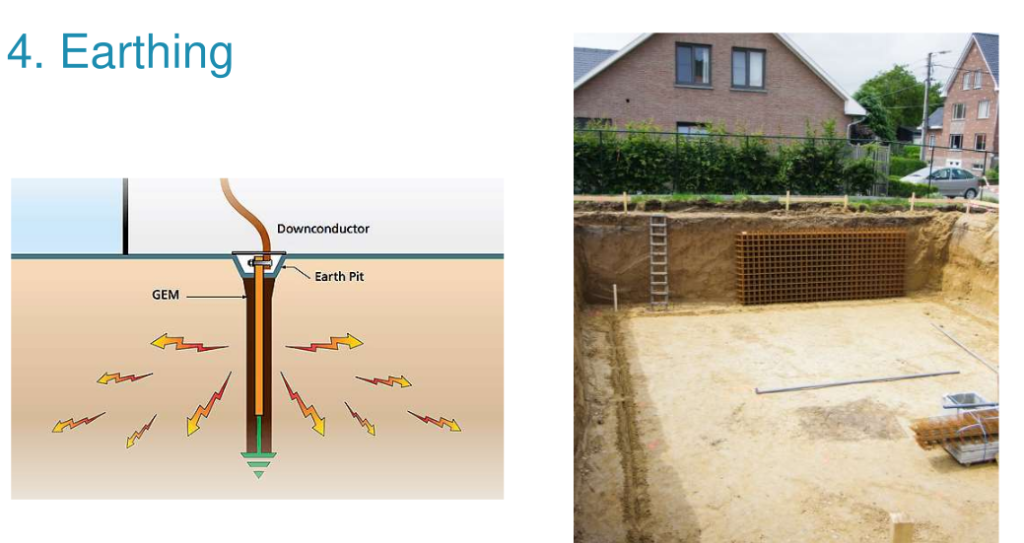
\includegraphics[width=\textwidth]{assets/earthing_aarding.png}
        \caption{Aardingsput met meetpen en funderingsaardlus.}
        \label{fig:earthing}
    \end{minipage}\hfill
    \begin{minipage}{0.48\textwidth}
        \centering
        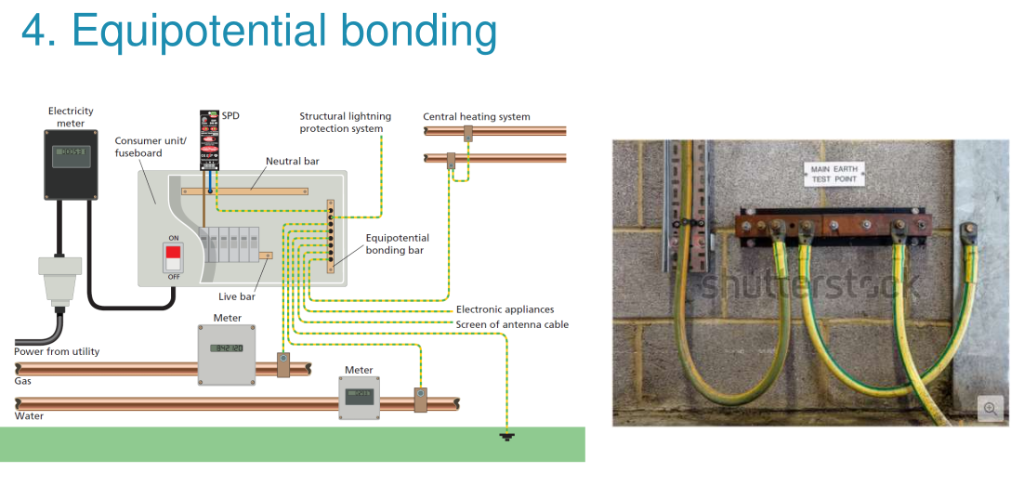
\includegraphics[width=\textwidth]{assets/equipotential_bonding.png}
        \caption{Equipotentiaalverbindingen van nutsvoorzieningen.}
        \label{fig:equipotential}
    \end{minipage}
\end{figure}
\FloatBarrier

\subsubsection{Aardlekschakelaar (RCD / Differentieel)}

\begin{conceptbox}[Aardlekschakelaar (RCD)]
    Een \keyterm{RCD} (Residual Current Device) is een beveiligingstoestel dat voortdurend de heen-
    en de terugstroom van een kring vergelijkt. Verdwijnt er stroom uit de kring --- de
    differentiaalstroom $I_\Delta$ --- dan lekt die naar de aarde, en schakelt het toestel uit zodra
    $I_\Delta$ de nominale aanspreekstroom $I_{\Delta n}$ bereikt.
\end{conceptbox}

\begin{wrapfigure}{r}{0.30\textwidth}
    \vspace{-4mm}
    \centering
    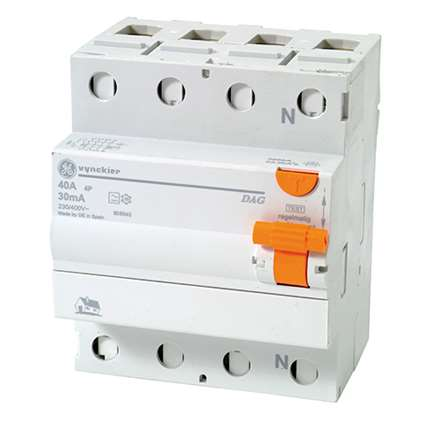
\includegraphics[width=0.28\textwidth]{assets/rcd_diff_foto.png}
    \caption{Een differentieel in de zekeringkast.}
    \label{fig:rcd-foto}
    \vspace{-3mm}
\end{wrapfigure}

Je komt hetzelfde toestel onder veel namen tegen: aardlekschakelaar, differentieelschakelaar,
verliesstroomschakelaar, RCCB of gewoon ``de differentieel''. In een Belgische woning zitten er
minstens twee, met een verschillende gevoeligheid, omdat ze twee verschillende dingen doen:

\begin{itemize}
    \item \textbf{Persoonsbeveiliging ($I_{\Delta n} = 30\text{ mA}$):} beschermt tegen elektrocutie,
          zowel bij rechtstreekse als bij onrechtstreekse aanraking. Verplicht op badkamer-, keuken-
          en buitenkringen.
    \item \textbf{Brandbeveiliging ($I_{\Delta n} = 300\text{ mA}$):} de algemene differentieel vooraan
          de installatie. Die moet geen mensen redden, maar voorkomen dat een sluipende isolatiefout
          de boel in brand zet door Joule-opwarming ($P = I_\Delta^2 R$).
\end{itemize}

Het meetprincipe is een \textbf{somstroomtransformator}: alle actieve geleiders (fase én nul) lopen
samen door één ringkern. In figuur~\ref{fig:rcd-werking-slide} zie je links de gezonde situatie
--- wat er langs de fase binnengaat, komt langs de nul terug, de som is nul --- en rechts een
aardfout, waarbij een deel van de stroom via de aarde wegvloeit en de som dus niet meer nul is.

\begin{figure}[htbp]
    \centering
    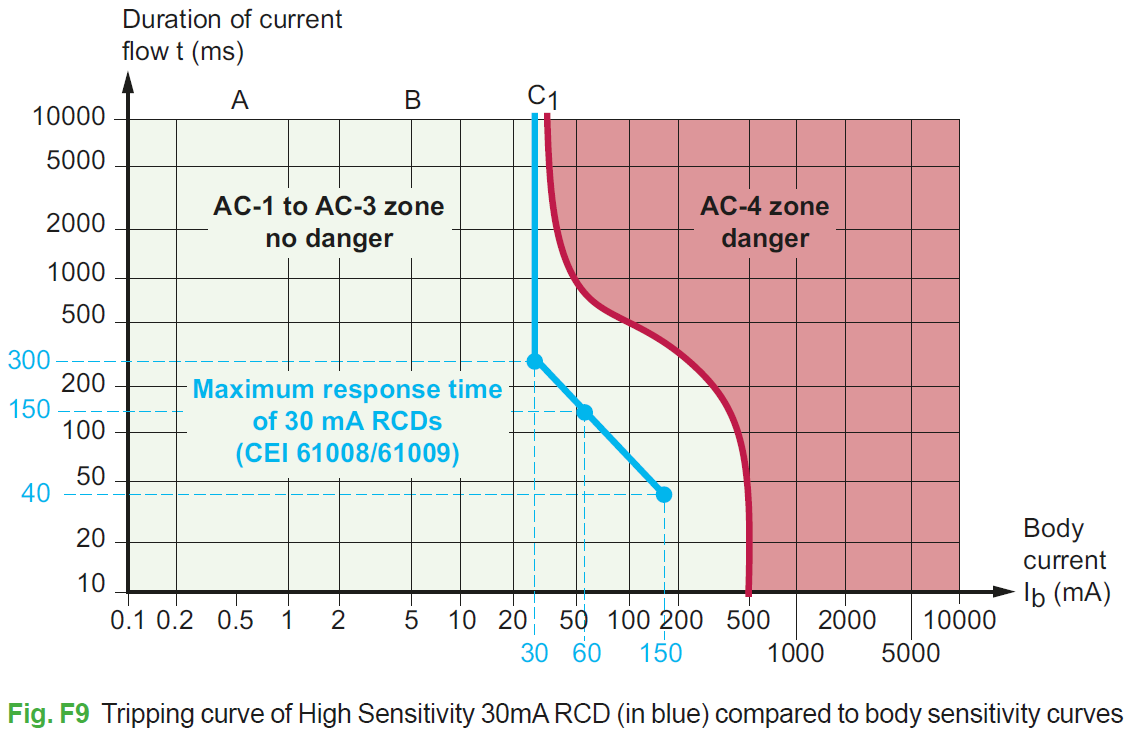
\includegraphics[width=0.85\textwidth]{assets/rcd_werking_schematisch.png}
    \caption{Werkingsprincipe van de RCD. Links: $i_L = i_N$, de somstroom door de ringkern is nul.
        Rechts: een deel van de stroom loopt via de aarde terug, de somstroom is niet meer nul en de
        RCD schakelt uit.}
    \label{fig:rcd-werking-slide}
\end{figure}
\FloatBarrier


\begin{center}
    \begin{tabular}{@{}p{30mm}p{45mm}p{45mm}@{}}
        \toprule
        \textbf{Toestand}               & \textbf{Stroombalans \& Magnetische flux}                                 & \textbf{Gevolg op uitschakelrelais}                                     \\
        \midrule
        \textbf{Normale werking}        & $i_L = i_N \implies \sum I = 0 \implies \Phi_{\text{net}} = 0$            & $e_{\text{sec}} = 0 \implies$ contacten blijven gesloten.               \\[1mm]
        \textbf{Aardlek / fout}         & $i_L - i_N = I_\Delta \ge I_{\Delta n} \implies \Phi_{\text{net}} \neq 0$ & $e_{\text{sec}} > 0 \implies$ relais ontgrendelt in $<30\text{ ms}$.    \\[1mm]
        \textbf{Testknop $T$ ingedrukt} & $I_T = U/R_T$ passeert slechts 1 keer door torus                          & Kunstmatige $\Phi_{\text{net}} \neq 0 \implies$ RCD tript ter controle. \\
        \bottomrule
    \end{tabular}
\end{center}

\textbf{Waarom exact $30\text{ mA}$ en $<30\text{ ms}$?}
Dit werkpunt is rechtstreeks afgeleid uit de IEC 60479-zonegrafiek (zie figuur~\ref{fig:ac-zones} en figuur~\ref{fig:rcd-tripping-curve}):
\begin{itemize}
    \item $30\text{ mA}$ ligt boven de loslaatdrempel ($10-15\text{ mA}$), maar bij een uitschakeltijd van
          $<30\text{ ms}$ bij zware fouten (en $<300\text{ ms}$ bij $I_{\Delta n}$) bevindt het werkpunt zich
          altijd in zone AC-2 / AC-3.
    \item De uitschakeling gebeurt hierdoor \textbf{ruim vóór curve $c_1$}, waardoor de kans op dodelijke
          ventrikelfibrillatie (zone AC-4) zo goed als uitgesloten is.
\end{itemize}

\textbf{Types RCD volgens aard van de foutstroom:}
\begin{itemize}
    \item \textbf{Type AC:} reageert enkel op zuivere sinusvormige wisselstromen (verouderd).
    \item \textbf{Type A:} reageert op sinusvormige wisselstromen én \textbf{pulserende gelijkstromen} (residentiële standaard volgens AREI).
    \item \textbf{Type B:} reageert op AC, pulserende DC én \textbf{gladde gelijkstromen} (PV-omvormers, laadpalen, frequentieregelaars).
\end{itemize}

\begin{waarschuwing}[Essentiële beperkingen van een RCD (Waar een RCD níet tegen beschermt)]
    \begin{enumerate}
        \item Een RCD biedt \belangrijk{geen bescherming tegen overbelasting of kortsluiting} tussen fase en nul!
              Loopt er $100\text{ A}$ tussen fase en nul zonder dat er stroom naar aarde lekt, dan is $\sum I = 0$
              en zal de RCD nooit trippen. Daarom moet een RCD altijd gecombineerd worden met een MCB.
        \item Een RCD reageert \textbf{niet} wanneer een persoon gelijktijdig de fase én de nulgeleider aanraakt
              zonder contact te maken met de aarde. De stroom vloeit dan zuiver van fase naar nul (voor de RCD is dit een gewone belasting).
    \end{enumerate}
\end{waarschuwing}



\section{Examenoefeningen}

Alle oefeningen hieronder komen uit echte examens. De bron staat er telkens bij.
Een uitgebreidere bundel met alle zittingen van 2022 tot 2026 vind je op studforum:
\url{https://wiki.studforum.net/pub/bac2/elektromagnetisme}

\begin{examenbox}
    Het examen bestaat altijd uit drie delen: \textbf{5 korte theorievragen}, \textbf{één 1-fase
        oefening} en \textbf{één 3-fase oefening}. De 1-fase en 3-fase oefening vragen bijna altijd
    ook een \textbf{fasordiagramma op schaal}. Vermeld je schaal expliciet (bv.\ 1:40 voor
    spanningen, 1:2 voor stromen), anders verlies je punten.
\end{examenbox}

\subsection{Fasors en impedanties}

\textbf{Opgave (20/01/2024 en 22/08/2024, theorievraag 1).}
Bereken de volgende uitdrukking in het fasordomein en zet ze terug naar het tijdsdomein:
\[5\cos(3t + 7^\circ) + 2\sin(3t - 28^\circ)\]

\begin{oefenblok}[Optellen van een sinus en een cosinus]

    \textbf{Stap 1: zet alles om naar dezelfde functie.}
    Je mag pas fasoren maken als beide termen dezelfde vorm hebben. Met $\sin\theta = \cos(\theta - 90^\circ)$:
    \[2\sin(3t - 28^\circ) = 2\cos(3t - 118^\circ)\]

    \begin{waarschuwing}[Dit is de valstrik]
        Een sinus en een cosinus mag je \textbf{niet} zomaar als fasor optellen. Zet ze eerst
        allebei om naar cosinus (of allebei naar sinus, maar wees consequent).
    \end{waarschuwing}

    \textbf{Stap 2: naar fasoren.}
    Beide termen hebben dezelfde pulsatie $\omega = 3$~rad/s, dus optellen mag:
    \[5\angle 7^\circ + 2\angle -118^\circ = (4{,}96 + j0{,}61) + (-0{,}94 - j1{,}77) = 4{,}02 - j1{,}16\]

    \textbf{Stap 3: terug naar polaire vorm.}
    \[4{,}02 - j1{,}16 = 4{,}19\angle -16^\circ\]

    \textbf{Stap 4: terug naar het tijdsdomein}, met dezelfde $\omega$:
    \[\boxed{4{,}19\cos(3t - 16^\circ)}\]

    Figuur~\ref{fig:fasor-optellen} toont dezelfde optelling grafisch: kop-staart, precies zoals je
    ze op het examen moet kunnen tekenen.
\end{oefenblok}

\begin{figure}[ht]
    \centering
    \begin{tikzpicture}[scale=1.0, >=latex]
        % assen
        \draw[->, gray!60] (-1.6,0) -- (6.4,0) node[right, font=\scriptsize, black] {Re};
        \draw[->, gray!60] (0,-2.6) -- (0,1.6) node[above, font=\scriptsize, black] {Im};
        % A = 5<7deg  -> (5.46, 0.67)
        \draw[->, very thick, schoolBlue] (0,0) -- (5.46,0.67)
        node[midway, above, font=\small, schoolBlue] {$5\angle 7^\circ$};
        % B = 2<-118deg, kop-staart vanaf tip A -> (4.43,-1.28)
        \draw[->, very thick, schoolOrange] (5.46,0.67) -- (4.43,-1.28)
        node[midway, right, font=\small, schoolOrange] {$2\angle -118^\circ$};
        % resultante
        \draw[->, ultra thick, schoolRed] (0,0) -- (4.42,-1.28)
        node[midway, below left, font=\small, schoolRed] {$4{,}19\angle -16^\circ$};
        % hoekje
        \draw[schoolRed, thin] (2.0,0) arc (0:-16:2.0);
        \node[font=\tiny, schoolRed, anchor=west] at (2.1,-0.32) {$-16^\circ$};
    \end{tikzpicture}
    \caption{Grafische optelling van de twee fasoren. De tweede fasor wordt kop-staart aan de eerste
        gehangen; de pijl van de oorsprong naar het eindpunt is de som.}
    \label{fig:fasor-optellen}
\end{figure}
\FloatBarrier

\textbf{Opgave (30/01/2025, theorievraag 3).}
Een niet-ideale spoel is een spoel in serie met een weerstand. De totale spanning erover is
$20$~V, de gemeten spanning over de spoel alleen is $10$~V, en $R = 5\,\Omega$. Bepaal $L$ bij
$50$~Hz.

\begin{figure}[ht]
    \centering
    \begin{circuitikz}[scale=0.9, transform shape]
        \draw (0,0) to[sV=$20\angle 0^\circ$~V, i>^=$\underline{I}$] (0,2.6);
        \draw (0,2.6) to[R, l_={$R = 5\,\Omega$}, v^>={$\underline{V}_R$}] (3.4,2.6);
        \draw (3.4,2.6) to[L, l_={$L = ?$}, v^>={$\underline{V}_L = 10$~V}] (6.8,2.6);
        \draw (6.8,2.6) -- (6.8,0) -- (0,0);
        \draw (0,0) node[ground]{};
    \end{circuitikz}
    \hspace{6mm}
    \begin{tikzpicture}[scale=0.16, >=latex, baseline=(current bounding box.center)]
        \draw[->, very thick, schoolBlue] (0,0) -- (17.32,0)
        node[midway, below, font=\scriptsize, schoolBlue] {$V_R = 17{,}32$~V};
        \draw[->, very thick, schoolOrange] (17.32,0) -- (17.32,10)
        node[midway, right, font=\scriptsize, schoolOrange] {$V_L = 10$~V};
        \draw[->, ultra thick, schoolRed] (0,0) -- (17.32,10)
        node[midway, above left, font=\scriptsize, schoolRed] {$V = 20$~V};
        \draw[gray!70] (15.6,0) -- (15.6,1.7) -- (17.32,1.7);
    \end{tikzpicture}
    \caption{Links het schema: een niet-ideale spoel is $R$ in serie met $L$. Rechts de
        spanningsdriehoek: $\underline{V}_R$ ligt in fase met de stroom, $\underline{V}_L$ staat er
        $90^\circ$ op, dus $V^2 = V_R^2 + V_L^2$.}
    \label{fig:oef-niet-ideale-spoel}
\end{figure}
\FloatBarrier

\begin{oefenblok}[Zelfinductie uit twee spanningsmetingen]

    \begin{waarschuwing}[Expliciete valstrik op het examen]
        De verleiding is om te rekenen als bij gelijkstroom: $V_R = 20 - 10 = 10$~V.
        \belangrijk{Dat is fout.} Dit is een wisselspanningsbron, dus je moet met fasehoeken werken.
    \end{waarschuwing}

    \textbf{Stap 1: gebruik dat $V_R$ en $V_L$ loodrecht op elkaar staan.}
    De stroom is gemeenschappelijk (serieschakeling). Over de weerstand ligt de spanning in fase
    met die stroom, over de spoel ijlt ze $90^\circ$ voor. De bronspanning is dus de
    \textbf{vectoriële} som:
    \[V^2 = V_R^2 + V_L^2 \quad\Rightarrow\quad V_R = \sqrt{20^2 - 10^2} = \sqrt{300} = 17{,}32\ \text{V}\]

    \textbf{Stap 2: de stroom volgt uit de weerstand.}
    \[I = \frac{V_R}{R} = \frac{17{,}32}{5} = 3{,}46\ \text{A}\]

    \textbf{Stap 3: de reactantie.}
    \[X_L = \frac{V_L}{I} = \frac{10}{3{,}46} = 2{,}89\ \Omega\]

    \textbf{Stap 4: de zelfinductie}, met $\omega = 2\pi \cdot 50 = 314{,}16$~rad/s:
    \[L = \frac{X_L}{\omega} = \frac{2{,}89}{314{,}16} = \boxed{9{,}19\ \text{mH}}\]

    \textbf{Kerninzicht.} De gelijkstroomredenering zou $X_L = 5\,\Omega$ en $L = 15{,}9$~mH geven:
    \textbf{73\% te veel}. Zodra er een spoel of condensator in het spel is, tellen spanningen
    nooit gewoon op.
\end{oefenblok}

\textbf{Opgave (15/01/2026, theorievraag 4).}
Een capacitieve belasting heeft $\cos\phi = 0{,}2588$ en een ohms deel van $1{,}34\,\Omega$.
Wat is de reactantie? Wat is het teken?

\begin{oefenblok}[Reactantie en teken uit de arbeidsfactor]

    \textbf{Stap 1: de hoek volgt uit de arbeidsfactor.}
    \[\phi = \arccos(0{,}2588) = 75^\circ\]

    \textbf{Stap 2: gebruik de impedantiedriehoek.}
    Voor een impedantie geldt $R = |Z|\cos\phi$ en $X = |Z|\sin\phi$, dus:
    \[X = R\tan\phi = 1{,}34 \cdot \tan 75^\circ = 1{,}34 \cdot 3{,}732 = 5{,}0\ \Omega\]

    \textbf{Stap 3: bepaal het teken.}
    \textbf{Capacitief} betekent dat de stroom voorijlt op de spanning, dus de fasehoek is negatief:
    \[\boxed{X = -5\ \Omega} \qquad Z = 1{,}34 - j5 = 5{,}18\angle -75^\circ\ \Omega\]

    \begin{examenbox}
        Onthoud de tekenregel: $Z_L = +j\omega L$ is altijd \textbf{positief}, $Z_C = -j/(\omega C)$
        is altijd \textbf{negatief}. Een negatieve reactantie is dus per definitie capacitief.
    \end{examenbox}
\end{oefenblok}

\begin{figure}[ht]
    \centering
    \begin{tikzpicture}[scale=0.85, >=latex]
        \draw[->, very thick, schoolBlue] (0,0) -- (1.34,0)
        node[midway, above, font=\scriptsize, schoolBlue] {$R = 1{,}34\,\Omega$};
        \draw[->, very thick, schoolOrange] (1.34,0) -- (1.34,-5)
        node[midway, right, font=\scriptsize, schoolOrange] {$X = -5\,\Omega$};
        \draw[->, ultra thick, schoolRed] (0,0) -- (1.34,-5)
        node[midway, left, font=\scriptsize, schoolRed] {$|Z| = 5{,}18\,\Omega$};
        \draw[schoolRed, thin] (0.9,0) arc (0:-75:0.9);
        \node[font=\scriptsize, schoolRed] at (1.35,-0.75) {$-75^\circ$};
        \draw[gray!70] (1.34,-0.32) -- (1.02,-0.32) -- (1.02,0);
    \end{tikzpicture}
    \caption{Impedantiedriehoek van de capacitieve belasting. Omdat de reactantie \emph{onder} de
        reële as ligt, is $X$ negatief en de hoek $\phi = -75^\circ$.}
    \label{fig:oef-impedantiedriehoek}
\end{figure}
\FloatBarrier

\subsection{Vermogen berekeningen}

\textbf{Opgave (18/01/2023, theorievraag b).}
Gegeven een fasordiagramma met $V = 200$~V onder $25^\circ$ en $I = 5$~A onder $-40^\circ$.
Geef het ogenblikkelijk vermogen en het actief vermogen.

\begin{figure}[ht]
    \centering
    \begin{tikzpicture}[scale=1.0, >=latex]
        \draw[->, gray!60] (-0.6,0) -- (4.8,0) node[right, font=\scriptsize, black] {Re};
        \draw[->, gray!60] (0,-2.4) -- (0,2.4) node[above, font=\scriptsize, black] {Im};
        % V = 200<25 graden, schaal 1 cm = 50 V
        \draw[->, very thick, schoolBlue] (0,0) -- (3.625,1.690)
        node[above right, font=\small, schoolBlue] {$\underline{V} = 200\angle 25^\circ$~V};
        % I = 5<-40 graden, schaal 1 cm = 1,79 A
        \draw[->, very thick, schoolOrange] (0,0) -- (2.145,-1.800)
        node[below right, font=\small, schoolOrange] {$\underline{I} = 5\angle -40^\circ$~A};
        % hoeken
        \draw[gray, thin] (1.2,0) arc (0:25:1.2);
        \node[font=\tiny, gray!50!black] at (1.42,0.26) {$25^\circ$};
        \draw[gray, thin] (1.0,0) arc (0:-40:1.0);
        \node[font=\tiny, gray!50!black] at (1.05,-0.45) {$-40^\circ$};
        \draw[schoolRed, thick] (2.1,0.98) arc (25:-40:2.32);
        \node[font=\small\bfseries, schoolRed] at (2.95,-0.32) {$\phi = 65^\circ$};
    \end{tikzpicture}
    \caption{Het gegeven fasordiagramma. Schalen: $1\text{ cm} = 50$~V en $1\text{ cm} = 1{,}79$~A.
        De stroom ijlt $65^\circ$ na op de spanning, dus de belasting is inductief.}
    \label{fig:oef-fasor-vermogen}
\end{figure}
\FloatBarrier

\begin{oefenblok}[Van fasordiagramma naar vermogen]

    \textbf{Stap 1: bepaal de faseverschuiving.}
    Dat is de hoek \textbf{van $V$ naar $I$}:
    \[\phi = 25^\circ - (-40^\circ) = 65^\circ\]

    \textbf{Stap 2: het ogenblikkelijk vermogen is het product van de tijdsfuncties.}
    Let op: hier gebruik je \textbf{piekwaarden}, niet de effectieve waarden.
    \[p(t) = v(t) \cdot i(t) = V_m\sin(\omega t + 25^\circ)\cdot I_m\sin(\omega t - 40^\circ)\]

    \textbf{Stap 3: werk uit met de goniometrische productformule}
    $\sin a\sin b = \tfrac{1}{2}[\cos(a-b) - \cos(a+b)]$:
    \[p(t) = VI\cos\phi - VI\cos(2\omega t - 15^\circ)\]
    Met $V$ en $I$ de effectieve waarden, $\phi$ de faseverschuiving en $\omega$ de pulsatie in rad/s.

    Het eerste stuk is \textbf{constant}, het tweede oscilleert met $2\omega$ en heeft gemiddelde nul.

    \textbf{Stap 4: het actief vermogen is het gemiddelde van $p(t)$.}
    \[P = VI\cos\phi = 200 \cdot 5 \cdot \cos 65^\circ = \boxed{422{,}6\ \text{W}}\]

    \textbf{Controle via het complex vermogen:}
    \[\underline{S} = \underline{V}\,\underline{I}^{*} = (200\angle 25^\circ)(5\angle +40^\circ) = 1000\angle 65^\circ\ \text{VA}\]
    \[P = 422{,}6\ \text{W} \qquad Q = 1000\sin 65^\circ = 906{,}3\ \text{VAR (inductief)}\]

    \begin{waarschuwing}[Vergeet de toegevoegde niet]
        $\underline{I}^{*}$ betekent dat je het \textbf{teken van de hoek omkeert}
        ($-40^\circ \rightarrow +40^\circ$). Doe je dat niet, dan krijg je $\phi = -15^\circ$ en een
        verkeerd vermogen.
    \end{waarschuwing}
\end{oefenblok}

\textbf{Opgave (15/01/2026, vraag 2).}
Een bron van $100$~V / $20$~Hz voedt een serie-impedantie $2+j3\,\Omega$, gevolgd door
$5+j2\,\Omega$ parallel met $3-j\,\Omega$.
Bepaal de arbeidsfactor van de hele keten, en welke condensator je parallel moet plaatsen om de
arbeidsfactor op $0{,}95$ te brengen.

\begin{figure}[ht]
    \centering
    \begin{circuitikz}[scale=0.9, transform shape]
        \draw (0,0) to[sV, l_={$100\angle 0^\circ$~V}] (0,3.2);
        \draw (0,3.2) to[generic=$2+j3\,\Omega$, i>^=$\underline{I}$] (3.4,3.2) node[circ]{};
        \draw (3.4,3.2) -- (6.0,3.2);
        \draw (3.4,3.2) to[generic=$5+j2\,\Omega$] (3.4,0);
        \draw (6.0,3.2) to[generic=$3-j\,\Omega$] (6.0,0) node[circ]{};
        \draw (0,0) -- (6.0,0);
        % correctiecondensator parallel met de bron
        \draw[dashed, schoolRed] (-3.2,0) to[C, l={$C$}, color=schoolRed] (-3.2,3.2);
        \draw[dashed, schoolRed] (-3.2,3.2) -- (0,3.2);
        \draw[dashed, schoolRed] (-3.2,0) -- (0,0);
        \node[font=\scriptsize, schoolRed, align=center] at (-3.2,-0.8) {correctie-\\condensator};
        \draw (0,0) node[ground]{};
    \end{circuitikz}
    \caption{Examen 15/01/2026, vraag 2. De serie-impedantie $2+j3\,\Omega$ staat vóór de
        parallelschakeling van $5+j2\,\Omega$ en $3-j\,\Omega$. De condensator voor
        arbeidsfactorcorrectie (rood, gestippeld) komt altijd \textbf{parallel met de bron}, nooit in
        serie.}
    \label{fig:oef-pf-correctie-circuit}
\end{figure}
\FloatBarrier

\begin{oefenblok}[Arbeidsfactorcorrectie]

    \textbf{Stap 1: werk de parallelschakeling uit.}
    \[\underline{Z}_p = \frac{(5+j2)(3-j)}{(5+j2)+(3-j)} = \frac{17+j}{8+j} = 2{,}11 - j0{,}14\ \Omega\]

    \textbf{Stap 2: totale impedantie.}
    \[\underline{Z}_{tot} = (2+j3) + (2{,}11 - j0{,}14) = 4{,}11 + j2{,}86 = 5{,}01\angle 34{,}9^\circ\ \Omega\]

    \textbf{Stap 3: de arbeidsfactor is de cosinus van de impedantiehoek.}
    \[\text{pf} = \cos 34{,}9^\circ = \boxed{0{,}82\ \text{naijlend}}\]

    \textbf{Stap 4: stroom en vermogens.}
    \[\underline{I} = \frac{100\angle 0^\circ}{5{,}01\angle 34{,}9^\circ} = 19{,}96\angle -34{,}9^\circ\ \text{A}\]
    \[\underline{S} = \underline{V}\,\underline{I}^{*} = 1996\angle 34{,}9^\circ\ \text{VA}
        \quad\Rightarrow\quad P = 1636\ \text{W},\ Q = 1142\ \text{VAR}\]

    \textbf{Stap 5: hoeveel reactief vermogen moet de condensator leveren?}
    Bij $\cos\phi_2 = 0{,}95$ hoort $\phi_2 = 18{,}2^\circ$. Het actief vermogen blijft gelijk:
    \[Q' = P\tan\phi_2 = 1636 \cdot 0{,}329 = 538\ \text{VAR}\]
    \[|Q_C| = Q - Q' = 1142 - 538 = 604\ \text{VAR}\]

    \textbf{Stap 6: de capaciteit}, met $\omega = 2\pi \cdot 20 = 125{,}7$~rad/s:
    \[C = \frac{|Q_C|}{V^2\omega} = \frac{604}{100^2 \cdot 125{,}7} = \boxed{481\ \mu\text{F}}\]

    \begin{waarschuwing}[Let op de frequentie]
        Hier is $f = 20$~Hz, niet $50$~Hz. Reken je automatisch met $\omega = 314$~rad/s, dan zit je
        een factor $2{,}5$ mis.
    \end{waarschuwing}

    \textbf{Controle: is de stroom effectief gedaald?}
    \[|S'| = \sqrt{1636^2 + 538^2} = 1722\ \text{VA} \quad\Rightarrow\quad I' = \frac{1722}{100} = 17{,}2\ \text{A}\]
    Dat is $14\%$ minder dan de oorspronkelijke $19{,}96$~A, bij exact hetzelfde nuttig vermogen.
    \textbf{Dat is de hele bedoeling van arbeidsfactorcorrectie:} minder stroom door de
    toevoerkabels, dus minder $I^2R$-verlies.
\end{oefenblok}

\begin{figure}[ht]
    \centering
    \begin{tikzpicture}[x=0.0029cm, y=0.0029cm, >=latex]
        % assen: 1 eenheid = 1 W of 1 VAR
        \draw[->, gray!60] (0,0) -- (1750,0) node[right, font=\scriptsize, black] {$P$ [W]};
        \draw[->, gray!60] (0,0) -- (0,1350) node[above, font=\scriptsize, black] {$Q$ [VAR]};
        % actief vermogen
        \draw[->, very thick, schoolBlue] (0,0) -- (1636,0);
        \node[font=\scriptsize, schoolBlue, below] at (818,-70) {$P = 1636$~W (blijft gelijk)};
        % reactief vermogen voor en na correctie
        \draw[->, very thick, schoolOrange] (1636,0) -- (1636,1142);
        % schijnbaar vermogen voor correctie
        \draw[->, ultra thick, schoolRed] (0,0) -- (1636,1142);
        \node[font=\scriptsize, schoolRed, anchor=south, rotate=34.9] at (700,489) {$|S| = 1996$~VA};
        % na correctie
        \draw[->, ultra thick, schoolGreen!55!black] (0,0) -- (1636,538);
        \node[font=\scriptsize, schoolGreen!45!black, anchor=north west, rotate=18.2] at (900,170) {$|S'| = 1722$~VA};
        % geleverd reactief vermogen van de condensator
        \draw[dashed, gray!70] (1636,538) -- (1990,538);
        \draw[dashed, gray!70] (1636,1142) -- (1990,1142);
        \draw[<->, thick, schoolPurple] (1730,538) -- (1730,1142);
        \node[font=\scriptsize, schoolPurple, anchor=south, rotate=90] at (1700,840) {$|Q_C| = 604$~VAR};
        \node[font=\scriptsize, schoolOrange, anchor=west] at (2010,1142) {$Q = 1142$~VAR};
        \node[font=\scriptsize, schoolGreen!45!black, anchor=west] at (2010,538) {$Q' = 538$~VAR};
        % hoeken
        \draw[schoolRed, thin] (620,0) arc (0:34.9:620);
        \node[font=\tiny, schoolRed, anchor=west] at (660,300) {$34{,}9^\circ$};
        \draw[schoolGreen!55!black, thin] (330,0) arc (0:18.2:330);
        \node[font=\tiny, schoolGreen!45!black, anchor=west] at (370,58) {$18{,}2^\circ$};
    \end{tikzpicture}
    \caption{Vermogendriehoek van de correctie. Het actief vermogen $P$ blijft ongewijzigd; de
        condensator levert $|Q_C|$ en duwt de top van de driehoek naar beneden, waardoor $|S|$ --- en
        dus de stroom --- daalt.}
    \label{fig:oef-pf-driehoek}
\end{figure}
\FloatBarrier

\textbf{Opgave (18/01/2023, theorievraag d).}
Er zijn twee driefasige belastingen op dezelfde generator aangesloten, met $P_1$, $Q_1$, $P_2$ en
$Q_2$. Wat is de arbeidsfactor van het gehele systeem?

\begin{oefenblok}[Arbeidsfactor van twee belastingen samen]

    \textbf{Stap 1: actieve en reactieve vermogens tellen gewoon op.}
    \[P_T = P_1 + P_2 \qquad Q_T = Q_1 + Q_2\]

    \textbf{Stap 2: het complex vermogen van het geheel.}
    \[\underline{S}_T = P_T + jQ_T\]

    \textbf{Stap 3: de arbeidsfactor is de cosinus van de hoek van $\underline{S}_T$.}
    \[\boxed{\cos\phi = \frac{P_T}{|\underline{S}_T|} = \frac{P_1+P_2}{\sqrt{(P_1+P_2)^2 + (Q_1+Q_2)^2}}}\]
    Met $P_T$ het totaal actief vermogen in W, $Q_T$ het totaal reactief vermogen in VAR en
    $|\underline{S}_T|$ het totaal schijnbaar vermogen in VA.

    \begin{waarschuwing}[Twee klassieke fouten]
        $|\underline{S}_T| \neq |S_1| + |S_2|$ en $\cos\phi_T \neq \tfrac{1}{2}(\cos\phi_1 + \cos\phi_2)$.
        Schijnbare vermogens zijn \textbf{vectoren}: je mag ze alleen complex optellen.
        Alleen $P$ en $Q$ zijn scalair optelbaar.
    \end{waarschuwing}
\end{oefenblok}

\subsection{AC circuit analyse}

\textbf{Opgave (18/01/2023, vraag 2).} Bepaal $\underline{I}$ en teken het fasorschema van alle
spanningen en stromen.

\begin{figure}[ht]
    \centering
    \begin{circuitikz}[scale=0.9, transform shape]
        \draw (0,0) to[sV=$8\angle 30^\circ$~V] (0,2.4);
        \draw (0,2.4) node[circ]{} node[above left]{$D$}
        to[R=$2\,\Omega$, i>^=$\underline{I}_3$] (3.6,2.4);
        \draw (3.6,2.4) node[circ]{} node[above]{$A$}
        to[L=$j2\,\Omega$, i>^=$\underline{I}_4$] (7.2,2.4) node[circ]{} node[above right]{$B$};
        \draw (3.6,2.4) to[C=$-j1\,\Omega$, i>^=$\underline{I}$] (3.6,0) node[circ]{} node[below]{$N$};
        \draw (0,0) -- (7.2,0);
        \draw (7.2,0) to[I=$1\angle 90^\circ$~A] (7.2,2.4);
        \draw (0,2.4) -- (0,4.4) to[C=$-j2\,\Omega$, i>^=$\underline{I}_5$] (3.6,4.4)
        to[L=$j4\,\Omega$] (7.2,4.4) -- (7.2,2.4);
        \draw (0,0) node[ground]{};
    \end{circuitikz}
    \caption{Examen 18/01/2023, vraag 2. Alle impedanties zijn al in $\Omega$ gegeven, dus je hebt
        geen frequentie nodig.}
    \label{fig:examen-2023-v2}
\end{figure}
\FloatBarrier

\begin{oefenblok}[Knooppuntanalyse met twee bronnen]

    \textbf{Stap 0: vereenvoudig eerst.} De bovenste tak bestaat uit twee elementen in serie:
    \[-j2 + j4 = j2\ \Omega\]
    Er loopt dus één spoel van $j2\,\Omega$ van $D$ naar $B$, parallel met de weg $D \to A \to B$.

    \textbf{Stap 1: kies de referentie.} Neem $N$ als aarde. Dan ligt $\underline{V}_D$ meteen vast:
    \[\underline{V}_D = 8\angle 30^\circ = 6{,}93 + j4\ \text{V}\]
    Er blijven twee onbekende knooppunten over ($A$ en $B$), dus je hebt \textbf{twee}
    KCL-vergelijkingen nodig.

    \textbf{Stap 2: KCL in knoop $A$} (som van de uitgaande stromen is nul):
    \[\frac{\underline{V}_A - \underline{V}_D}{2} + \frac{\underline{V}_A - 0}{-j} + \frac{\underline{V}_A - \underline{V}_B}{j2} = 0\]

    \textbf{Stap 3: KCL in knoop $B$.} De stroombron duwt $1\angle 90^\circ$ \emph{in} $B$:
    \[\frac{\underline{V}_B - \underline{V}_A}{j2} + \frac{\underline{V}_B - \underline{V}_D}{j2} - 1\angle 90^\circ = 0\]

    \textbf{Stap 4: los het stelsel op} (rekenmachine in complexe modus):
    \[\underline{V}_A = 3{,}46 - j3{,}65\ \text{V} \qquad \underline{V}_B = 4{,}19 + j0{,}18\ \text{V}\]

    \textbf{Stap 5: de gevraagde stroom} volgt uit de wet van Ohm over de condensator:
    \[\underline{I} = \frac{\underline{V}_A}{-j} = 3{,}65 + j3{,}46 = \boxed{5{,}03\angle 43{,}5^\circ\ \text{A}}\]

    \textbf{Stap 6: de overige takstromen} (nodig voor het fasordiagramma):
    \[\underline{I}_3 = \frac{\underline{V}_D - \underline{V}_A}{2} = 4{,}20\angle 65{,}6^\circ\ \text{A}\]
    \[\underline{I}_4 = \frac{\underline{V}_A - \underline{V}_B}{j2} = 1{,}95\angle 169^\circ\ \text{A}\]
    \[\underline{I}_5 = \frac{\underline{V}_D - \underline{V}_B}{j2} = 2{,}35\angle -35{,}6^\circ\ \text{A}\]

    \textbf{Controle.} KCL moet kloppen in beide knopen:
    \[\underline{I}_3 = \underline{I} + \underline{I}_4 \quad\checkmark \qquad
        \underline{I}_4 + \underline{I}_5 + 1\angle 90^\circ = 0 \quad\checkmark\]

    \textbf{Het fasordiagramma tekenen.} Zet $N$ in de oorsprong en teken $\underline{V}_{DN}$,
    $\underline{V}_{AN}$ en $\underline{V}_{BN}$ vanuit $N$. De punten $D$, $A$ en $B$ zijn dan de
    pijlpunten, en de zijden $DA$, $AB$ en $DB$ van die driehoek zijn automatisch de takspanningen.
    De stromen teken je vanuit hetzelfde punt met een eigen schaal.
\end{oefenblok}

\textbf{Opgave (13/01/2025, vraag 1).} Gegeven het net hieronder met $|\underline{I}| = 25{,}3$~A,
$|\underline{I}_C| = 40$~A, $|\underline{I}_L| = 17{,}9$~A en $f = 100$~Hz.
Bepaal $R$ en $L$, de bronspanning, $P$ en $Q$, en de arbeidsfactor.

\begin{figure}[ht]
    \centering
    \begin{circuitikz}[scale=0.9, transform shape]
        \draw (0,0) to[sV=$\underline{V}_s$, i<^=$\underline{I}$] (0,3.4);
        \draw (0,3.4) node[circ]{} node[above]{$B$} to[R=$5\,\Omega$] (3.4,3.4);
        \draw (3.4,3.4) node[circ]{} node[above]{$D$}
        to[C=$-j3\,\Omega$, i>^=$\underline{I}_C$] (3.4,0);
        \draw (3.4,3.4) -- (6.4,3.4) to[R=$R$, i>^=$\underline{I}_L$] (6.4,1.8);
        \draw (6.4,1.8) node[circ]{} node[right]{$E$} to[L=$L$] (6.4,0);
        \draw (0,0) node[circ]{} node[below]{$A$} -- (6.4,0);
        \draw (0,0) node[ground]{};
    \end{circuitikz}
    \caption{Examen 13/01/2025, vraag 1. Van de stromen ken je enkel de grootte, niet de hoek.}
    \label{fig:examen-2025-v1}
\end{figure}
\FloatBarrier

\begin{oefenblok}[Cosinusregel wanneer je enkel stroomgrootten kent]

    \begin{examenbox}
        Zodra je alleen \textbf{grootten} van stromen krijgt die samen een KCL-knoop vormen, is de
        \textbf{cosinusregel} de sleutel. De drie fasoren vormen dan een gesloten driehoek.
    \end{examenbox}

    \textbf{Stap 1: kies $\underline{I}$ als referentie:} $\underline{I} = 25{,}3\angle 0^\circ$~A.
    KCL in knoop $D$ geeft:
    \[\underline{I} = \underline{I}_C + \underline{I}_L\]

    \textbf{Stap 2: cosinusregel} voor de hoek $\theta_1$ tussen $\underline{I}$ en
    $\underline{I}_C$ (die staat tegenover zijde $|I_L|$):
    \[\cos\theta_1 = \frac{|I|^2 + |I_C|^2 - |I_L|^2}{2|I||I_C|}
        = \frac{25{,}3^2 + 40^2 - 17{,}9^2}{2 \cdot 25{,}3 \cdot 40} = 0{,}9485
        \ \Rightarrow\ \theta_1 = 18{,}48^\circ\]

    \textbf{Stap 3: idem voor de hoek tussen $\underline{I}$ en $\underline{I}_L$:}
    \[\cos\theta_3 = \frac{|I|^2 + |I_L|^2 - |I_C|^2}{2|I||I_L|} = -0{,}7061
        \ \Rightarrow\ \theta_3 = 134{,}91^\circ\]
    \[\underline{I}_C = 40\angle 18{,}48^\circ\ \text{A} \qquad
        \underline{I}_L = 17{,}9\angle -134{,}91^\circ\ \text{A}\]

    \textbf{Controle:} $\underline{I}_C + \underline{I}_L = 25{,}29 + j0{,}01 \approx 25{,}3\angle 0^\circ$ \checkmark

    \textbf{Waarom ligt $\underline{I}_C$ boven en $\underline{I}_L$ onder?} Een condensator laat de
    stroom voorijlen op de spanning, een spoel laat hem naijlen. Beide takken staan over dezelfde
    $\underline{V}_D$, dus hun stromen liggen aan weerszijden ervan.

    \textbf{Stap 4: de spanningen}, van links naar rechts:
    \[\underline{V}_{BD} = 5\underline{I} = 126{,}5\angle 0^\circ\ \text{V}\]
    \[\underline{V}_D = \underline{I}_C \cdot (-j3) = 120\angle -71{,}52^\circ\ \text{V}\]

    \textbf{Stap 5: de bronspanning} is de som van beide spanningsvallen:
    \[\underline{V}_s = \underline{V}_{BD} + \underline{V}_D = 164{,}4 - j113{,}8 = \boxed{200\angle -34{,}7^\circ\ \text{V}}\]

    \textbf{Stap 6: $R$ en $L$.} De RL-tak draagt $\underline{I}_L$ en staat over $\underline{V}_D$:
    \[R + j\omega L = \frac{\underline{V}_D}{\underline{I}_L}
        = \frac{120\angle -71{,}52^\circ}{17{,}9\angle -134{,}91^\circ} = 6{,}70\angle 63{,}39^\circ\ \Omega\]
    \[R = 6{,}70\cos 63{,}39^\circ = \boxed{3\ \Omega} \qquad \omega L = 6{,}70\sin 63{,}39^\circ = 5{,}99\ \Omega\]
    Met $\omega = 2\pi \cdot 100 = 628{,}3$~rad/s:
    \[L = \frac{5{,}99}{628{,}3} = \boxed{9{,}53\ \text{mH}}\]

    \begin{waarschuwing}[Doe dit niet met een stelsel]
        Als je $R$ en $L$ apart als onbekenden invoert, krijg je een derdegraadsvergelijking.
        \textbf{Eén enkele complexe deling volstaat.}
    \end{waarschuwing}

    \textbf{Stap 7: vermogens en arbeidsfactor.}
    \[\underline{S} = \underline{V}_s\underline{I}^{*} = 200\angle -34{,}7^\circ \cdot 25{,}3\angle 0^\circ
        = 5060\angle -34{,}7^\circ\ \text{VA}\]
    \[P = \boxed{4160\ \text{W}} \qquad Q = \boxed{-2881\ \text{VAR}} \qquad
        \text{pf} = \frac{4160}{5060} = \boxed{0{,}822\ \text{voorijlend}}\]

    \textbf{Waarom capacitief?} $|I_C| = 40$~A is veel groter dan $|I_L| = 17{,}9$~A: de condensator
    domineert, de stroom ijlt voor op de spanning, dus $Q < 0$.
\end{oefenblok}

\subsection{3-fase systemen}

\textbf{Gemengde driefasige lasten.} Een losse impedantie tussen twee lijnen vormt geen fase
van een sterlast. Reken die tak \textbf{apart} met de lijnspanning en tel haar stroom daarna
met KCL bij de twee betrokken lijnstromen. Bijgevolg kan één lijnstroom onveranderd blijven,
terwijl de andere twee veranderen:
\[
\underline{I}_{bc}=\frac{\underline{V}_{bc}}{\underline{Z}_{bc}},\qquad
\underline{I}_b=\underline{I}_{bY}+\underline{I}_{bc},\qquad
\underline{I}_c=\underline{I}_{cY}-\underline{I}_{bc}
\]
met: $\underline{I}_{bc}$ = stroom door de losse tak van $b$ naar $c$ (A),
$\underline{I}_{bY}$ en $\underline{I}_{cY}$ = stromen van de sterlast (A), en
$\underline{V}_{bc}$ = lijnspanning (V).

\textbf{Controle:} ook bij deze ongebalanceerde belasting moet
$\underline{I}_a+\underline{I}_b+\underline{I}_c=0$ gelden. Tel vermogens op via $P$ en $Q$,
niet via de groottes van de schijnbare vermogens.

\textbf{Opgave (18/01/2023, vraag 3).} Een evenwichtige bron van $208$~V met $\underline{V}_{ab}$
als referentie voedt een ongebalanceerde driehoekbelasting. Bepaal de lijnstromen en het totale
actief vermogen, sluit de 2-wattmetermethode aan en bereken beide aflezingen.

\begin{figure}[ht]
    \centering
    \begin{tikzpicture}[scale=1.0, line width=0.7pt]
        \coordinate (A) at (2.6,2.6); \coordinate (B) at (0.6,0); \coordinate (C) at (4.6,0);
        \draw (A)--(B) node[midway,sloped,fill=white,inner sep=1.2pt]{$30\,\Omega$};
        \draw (A)--(C) node[midway,sloped,fill=white,inner sep=1.2pt]{$90\,\Omega$};
        \draw (B)--(C) node[midway,fill=white,inner sep=1.2pt]{$60\,\Omega$};
        \fill (A) circle(1.6pt) node[above]{$A$};
        \fill (B) circle(1.6pt) node[below left]{$B$};
        \fill (C) circle(1.6pt) node[below right]{$C$};
        \draw[-{Latex[length=2mm]}] (-1.4,2.6) -- (A) node[midway,above]{$\underline{I}_a$};
        \draw[-{Latex[length=2mm]}] (-1.4,0) -- (B) node[midway,above]{$\underline{I}_b$};
        \draw[-{Latex[length=2mm]}] (-1.4,-1.0) -- (4.6,-1.0) -- (C) node[pos=0.25,below]{$\underline{I}_c$};
        \node[left] at (-1.4,2.6){$a$}; \node[left] at (-1.4,0){$b$}; \node[left] at (-1.4,-1.0){$c$};
    \end{tikzpicture}
    \caption{Examen 18/01/2023, vraag 3: zuiver ohmse, \emph{ongebalanceerde} driehoekbelasting op
        een evenwichtig 208~V-net.}
    \label{fig:examen-2023-v3}
\end{figure}
\FloatBarrier

\begin{oefenblok}[Ongebalanceerde driehoek met twee wattmeters]

    \textbf{Stap 1: de lijnspanningen} (abc-volgorde, $\underline{V}_{ab}$ als referentie):
    \[\underline{V}_{ab} = 208\angle 0^\circ \quad
        \underline{V}_{bc} = 208\angle -120^\circ \quad
        \underline{V}_{ca} = 208\angle 120^\circ\ \text{V}\]
    Bij een driehoek is $V_f = V_L$, dus dit zijn meteen ook de spanningen over de weerstanden.

    \textbf{Stap 2: de fasestromen} met de wet van Ohm per tak:
    \[\underline{I}_{AB} = \frac{208\angle 0^\circ}{30} = 6{,}93\angle 0^\circ\ \text{A}\]
    \[\underline{I}_{BC} = \frac{208\angle -120^\circ}{60} = 3{,}47\angle -120^\circ\ \text{A}\]
    \[\underline{I}_{CA} = \frac{208\angle 120^\circ}{90} = 2{,}31\angle 120^\circ\ \text{A}\]

    \begin{waarschuwing}[Ongebalanceerd]
        De belasting is ongebalanceerd, dus je mag \textbf{niet} één fase uitrekenen en
        $\pm 120^\circ$ draaien. Elke tak moet apart.
    \end{waarschuwing}

    \textbf{Stap 3: de lijnstromen} met KCL in de hoekpunten:
    \[\underline{I}_a = \underline{I}_{AB} - \underline{I}_{CA} = 8{,}09 - j2{,}00 = \boxed{8{,}33\angle -13{,}9^\circ\ \text{A}}\]
    \[\underline{I}_b = \underline{I}_{BC} - \underline{I}_{AB} = -8{,}67 - j3{,}00 = \boxed{9{,}17\angle -160{,}9^\circ\ \text{A}}\]
    \[\underline{I}_c = \underline{I}_{CA} - \underline{I}_{BC} = 0{,}58 + j5{,}00 = \boxed{5{,}04\angle 83{,}4^\circ\ \text{A}}\]

    \textbf{Controle:} bij een driehoek zonder nulgeleider moet gelden
    $\underline{I}_a + \underline{I}_b + \underline{I}_c = 0$ \checkmark

    \textbf{Stap 4: totaal actief vermogen.} Alle takken zijn ohms, dus $\cos\phi = 1$:
    \[P_{tot} = \frac{V_L^2}{R_{AB}} + \frac{V_L^2}{R_{BC}} + \frac{V_L^2}{R_{CA}}
        = 208^2\left(\tfrac{1}{30} + \tfrac{1}{60} + \tfrac{1}{90}\right) = \boxed{2644\ \text{W}}\]
    Er is geen reactief vermogen: $Q_{tot} = 0$ en dus $\text{pf} = 1$.

    \textbf{Stap 5: de 2-wattmetermethode aansluiten.}
    Wattmeter $W_1$: stroomspoel in lijn $a$, spanningsspoel tussen $a$ en $b$.
    Wattmeter $W_2$: stroomspoel in lijn $c$, spanningsspoel tussen $c$ en $b$.
    Lijn $b$ is dus het \textbf{gemeenschappelijke referentiepunt}: daar staat géén wattmeter.

    \textbf{Stap 6: de aflezingen} zijn het reële deel van $\underline{V}\,\underline{I}^{*}$:
    \[W_1 = \text{Re}\{\underline{V}_{ab}\underline{I}_a^{*}\} = 208 \cdot 8{,}33 \cdot \cos(0^\circ + 13{,}9^\circ) = \boxed{1682\ \text{W}}\]
    \[W_2 = \text{Re}\{\underline{V}_{cb}\underline{I}_c^{*}\} = 208 \cdot 5{,}04 \cdot \cos(60^\circ - 83{,}4^\circ) = \boxed{962\ \text{W}}\]

    \begin{waarschuwing}[Klassieke tekenfout]
        $\underline{V}_{cb} = -\underline{V}_{bc} = 208\angle 60^\circ$, \textbf{niet}
        $208\angle -120^\circ$. Dit teken is dé fout in deze vraag.
    \end{waarschuwing}

    \textbf{Stap 7: controle.} De som moet gelijk zijn aan stap 4:
    \[P_{tot} = W_1 + W_2 = 1682 + 962 = 2644\ \text{W} \quad\checkmark\]

    \textbf{Waarom werken twee wattmeters?} Uit KCL volgt
    $\underline{I}_b = -(\underline{I}_a + \underline{I}_c)$: de derde lijnstroom bevat geen extra
    informatie. Meet je twee lijnstromen ten opzichte van dezelfde referentielijn, dan zit daar alle
    informatie over het totale actief vermogen in, \textbf{ook bij onevenwicht}, en ook als de last
    in ster of in driehoek staat. Wél geldt dan: één wattmeter meet níet het vermogen van één fase,
    alleen de som heeft betekenis. En $Q_{tot} = \sqrt{3}(W_2 - W_1)$ geldt \textbf{enkel bij
        een evenwichtig systeem}.
\end{oefenblok}

\textbf{Opgave (13/01/2025, vraag 2).} Een evenwichtige sterbelasting heeft een totaal schijnbaar
vermogen van $150$~kVA bij $\text{pf} = 0{,}906$ (naijlend). Daarnaast hangt er één losse impedantie
$\underline{Z} = -j3\,\Omega$ tussen de lijnen $a$ en $b$. Het net is $3\times 200$~V, volgorde
$a$-$b$-$c$. Bepaal de lijnstromen, $P$ en $Q$ van de bron, en de totale arbeidsfactor.

\begin{oefenblok}[Evenwichtige ster met één extra last ertussen]

    \begin{examenbox}
        \textbf{Kernidee:} dit net is de \textbf{superpositie} van een evenwichtige sterlast en één
        losse tak tussen twee lijnen. Reken beide apart uit en tel de stromen op met KCL.
    \end{examenbox}

    \textbf{Stap 1: de evenwichtige sterlast.} Uit $S = \sqrt{3}V_L I_L$:
    \[I_L = \frac{150 \cdot 10^3}{\sqrt{3} \cdot 200} = 433{,}01\ \text{A}
        \qquad \phi = \arccos(0{,}906) = 25^\circ\]
    Bij een ster geldt $\underline{V}_L = \sqrt{3}\,\underline{V}_f\angle 30^\circ$, dus
    $\underline{V}_{aN} = 115{,}5\angle -30^\circ$~V. De fasestroom ijlt $25^\circ$ na:
    \[\underline{I}_{aN} = 433{,}01\angle -55^\circ \quad
        \underline{I}_{bN} = 433{,}01\angle -175^\circ \quad
        \underline{I}_{cN} = 433{,}01\angle 65^\circ\ \text{A}\]

    \textbf{Stap 2: de losse tak} staat over de volle lijnspanning:
    \[\underline{I}_{AB} = \frac{\underline{V}_{ab}}{-j3} = \frac{200\angle 0^\circ}{3\angle -90^\circ} = 66{,}67\angle 90^\circ\ \text{A}\]

    \textbf{Stap 3: KCL per lijn.} $\underline{I}_{AB}$ vertrekt uit $a$ en komt aan in $b$:
    \[\underline{I}_a = \underline{I}_{aN} + \underline{I}_{AB} = \boxed{380{,}3\angle -49{,}2^\circ\ \text{A}}\]
    \[\underline{I}_b = \underline{I}_{bN} - \underline{I}_{AB} = \boxed{443{,}8\angle -166{,}4^\circ\ \text{A}}\]
    \[\underline{I}_c = \underline{I}_{cN} = \boxed{433{,}0\angle 65^\circ\ \text{A}}\]

    \begin{waarschuwing}[Let op het teken]
        In lijn $a$ komt de extra stroom \textbf{bij}, in lijn $b$ gaat hij \textbf{af}. Lijn $c$
        voelt niets van de extra last. Precies daardoor is het systeem nu ongebalanceerd.
    \end{waarschuwing}

    \textbf{Stap 4: de vermogens.} De evenwichtige ster:
    \[\underline{S}_Y = 150\angle 25^\circ = 136{,}0 + j63{,}4\ \text{kVA}\]
    De losse capacitieve tak is zuiver reactief ($P = 0$):
    \[\underline{S}_Z = \frac{|V_{ab}|^2}{\underline{Z}^{*}} = \frac{200^2}{+j3} = -j13{,}33\ \text{kVA}\]
    Optellen mag, want $P$ en $Q$ zijn scalair optelbaar:
    \[\underline{S}_{tot} = 136{,}0 + j(63{,}4 - 13{,}3) = \boxed{136{,}0 + j50{,}1\ \text{kVA}}\]

    \textbf{Stap 5: de totale arbeidsfactor.}
    \[|\underline{S}_{tot}| = 144{,}9\ \text{kVA} \qquad
        \text{pf} = \frac{136{,}0}{144{,}9} = \boxed{0{,}94\ \text{naijlend}}\]

    \textbf{De condensatortak heeft de arbeidsfactor verbeterd} van $0{,}906$ naar $0{,}94$ --- dat
    is precies wat een compensatiecondensator doet: hij levert reactief vermogen dat de spoelen
    anders van het net zouden trekken.
\end{oefenblok}

\subsection{3-fase vermogen}


\begin{figure}[ht]
    \centering
    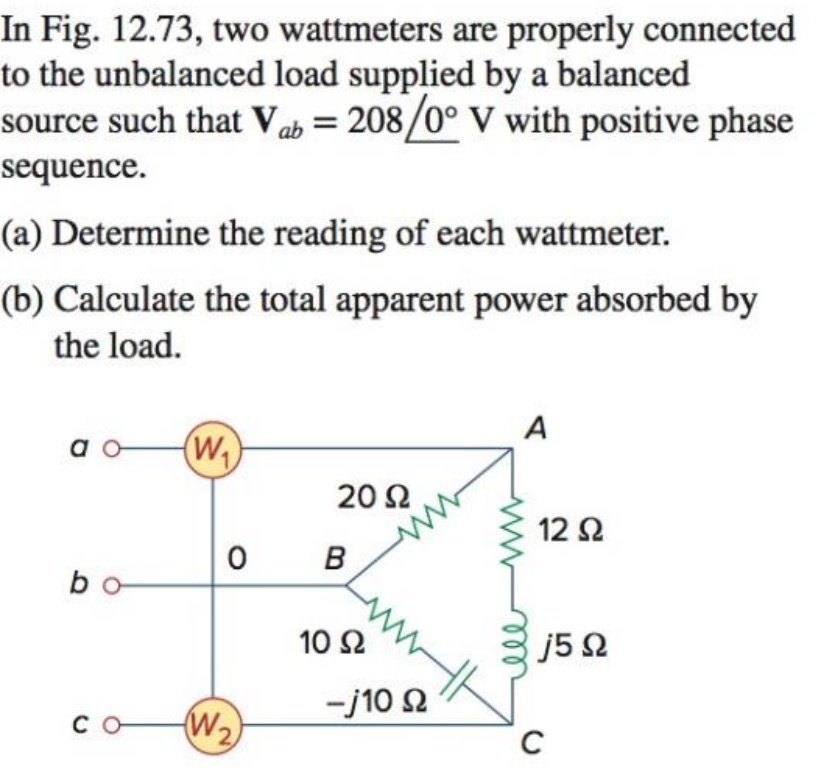
\includegraphics[width=0.4\textwidth]{assets/examen1.png}
    \caption{Schema bij de examenoefening over de ongebalanceerde Delta-belasting.}
    \label{fig:examen1.png}
\end{figure}

\textbf{Opgave: Ongebalanceerde Delta-belasting met twee-wattmetermethode}

Een ongebalanceerde Delta-verbonden belasting wordt gevoed door een evenwichtige bron met positieve fasevolgorde.

\textbf{Gegeven:}
\begin{itemize}
    \item Bronspanning: $\mathbf{V}_{ab} = 208\angle{0^\circ} \text{ V}$ (positieve fasevolgorde $abc$)
    \item Belastingsimpedanties:
          \begin{itemize}
              \item $\mathbf{Z}_{AB} = 20 \, \Omega$
              \item $\mathbf{Z}_{BC} = 10 - j10 \, \Omega$
              \item $\mathbf{Z}_{CA} = 12 + j5 \, \Omega$
          \end{itemize}
\end{itemize}

\textbf{Gevraagd:}
\begin{enumerate}
    \item (a) Bepaal de aflezingen van beide wattmeters in de twee-wattmetermethode
    \item (b) Bereken het totale schijnbare vermogen dat door de belasting wordt opgenomen
\end{enumerate}

\begin{oefenblok}[Ongebalanceerde Delta-belasting analyse]

    \textbf{Gegeven bronspanningen} (positieve fasevolgorde):
    \begin{align*}
        \mathbf{V}_{ab} & = 208\angle{0^\circ} \text{ V}    \\
        \mathbf{V}_{bc} & = 208\angle{-120^\circ} \text{ V} \\
        \mathbf{V}_{ca} & = 208\angle{120^\circ} \text{ V}
    \end{align*}

    \textbf{Stap 1: Bereken de fasestromen in de Delta-belasting}

    Met behulp van de wet van Ohm berekenen we de stromen in elk been van de Delta ($\mathbf{I} = \mathbf{V}/\mathbf{Z}$).

    \textbf{Stroom AB:}
    $$\mathbf{I}_{AB} = \frac{\mathbf{V}_{ab}}{\mathbf{Z}_{AB}} = \frac{208\angle{0^\circ}}{20} = 10.4\angle{0^\circ} \text{ A}$$

    \textbf{Stroom BC:}
    Eerst zetten we $\mathbf{Z}_{BC} = 10 - j10$ om naar poolcoördinaten:
    $$|\mathbf{Z}_{BC}| = \sqrt{10^2 + 10^2} = 14.14 \text{ } \Omega, \quad \theta = \tan^{-1}(-1) = -45^\circ$$
    $$\mathbf{Z}_{BC} = 14.14\angle{-45^\circ} \text{ } \Omega$$

    $$\mathbf{I}_{BC} = \frac{\mathbf{V}_{bc}}{\mathbf{Z}_{BC}} = \frac{208\angle{-120^\circ}}{14.14\angle{-45^\circ}} = 14.71\angle{-75^\circ} \text{ A}$$

    Gewoon in je rekenmachine zetten in r<theta modus.

    In rechthoekige vorm: $3.81 - j14.21 \text{ A}$

    \textbf{Stroom CA:}
    Eerst zetten we $\mathbf{Z}_{CA} = 12 + j5$ om naar poolcoördinaten:
    $$|\mathbf{Z}_{CA}| = \sqrt{12^2 + 5^2} = 13 \text{ } \Omega, \quad \theta = \tan^{-1}(5/12) = 22.62^\circ$$
    $$\mathbf{Z}_{CA} = 13\angle{22.62^\circ} \text{ } \Omega$$

    $$\mathbf{I}_{CA} = \frac{\mathbf{V}_{ca}}{\mathbf{Z}_{CA}} = \frac{208\angle{120^\circ}}{13\angle{22.62^\circ}} = 16\angle{97.38^\circ} \text{ A}$$

    In rechthoekige vorm: $-2.06 + j15.87 \text{ A}$

    \textbf{Stap 2: Bereken de lijnstromen met Kirchhoff}

    Met de knooppuntswet (KCL):

    \textbf{Lijnstroom $\mathbf{I}_a$:}
    $$\mathbf{I}_a = \mathbf{I}_{AB} - \mathbf{I}_{CA} = 10.4 - (-2.06 + j15.87) = 12.46 - j15.87 \text{ A}$$

    In poolcoördinaten:
    $$\mathbf{I}_a = 20.17\angle{-51.87^\circ} \text{ A}$$

    \textbf{Lijnstroom $\mathbf{I}_c$:}
    $$\mathbf{I}_c = \mathbf{I}_{CA} - \mathbf{I}_{BC} = (-2.06 + j15.87) - (3.81 - j14.21) = -5.87 + j30.08 \text{ A}$$

    In poolcoördinaten (2e kwadrant):
    $$\mathbf{I}_c = 30.65\angle{101.04^\circ} \text{ A}$$

    \textbf{Stap 3: Bepaal de wattmeteraflezing}

    \textbf{Wattmeter 1 ($W_1$):} Meet stroom $\mathbf{I}_a$ en spanning $\mathbf{V}_{ab}$
    $$P_1 = |\mathbf{V}_{ab}| \cdot |\mathbf{I}_a| \cdot \cos(0^\circ - (-51.87^\circ)) = 208 \times 20.17 \times \cos(51.87^\circ)$$
    $$\boxed{P_1 = 208 \times 20.17 \times 0.6175 = \mathbf{2590.6 \text{ W}}}$$

    \textbf{Wattmeter 2 ($W_2$):} Meet stroom $\mathbf{I}_c$ en spanning $\mathbf{V}_{cb}$

    Opmerking: $\mathbf{V}_{cb} = -\mathbf{V}_{bc} = 208\angle{60^\circ}$

    $$P_2 = |\mathbf{V}_{cb}| \cdot |\mathbf{I}_c| \cdot \cos(60^\circ - 101.04^\circ) = 208 \times 30.65 \times \cos(-41.04^\circ)$$
    $$\boxed{P_2 = 208 \times 30.65 \times 0.7543 = \mathbf{4808.6 \text{ W}}}$$

    \textbf{Onderdeel (a): Wattmeteraflezing}
    \begin{itemize}
        \item $W_1 = 2590.6 \text{ W}$ (of ongeveer 2.59 kW)
        \item $W_2 = 4808.6 \text{ W}$ (of ongeveer 4.81 kW)
        \item Totaal actief vermogen: $P_{\text{totaal}} = W_1 + W_2 = 7399.2 \text{ W}$
    \end{itemize}

    \textbf{Stap 4: Bereken het totale schijnbare vermogen}

    We berekenen het complex vermogen van elke belasting afzonderlijk:

    \textbf{Belasting AB:}
    $$\boxed{\mathbf{S}_{AB} = |\mathbf{I}_{AB}|^2 \times \mathbf{Z}_{AB} = 10.4^2 \times 20 = 2163.2 \text{ VA}}$$

    \textbf{Belasting BC:}
    $$\mathbf{S}_{BC} = |\mathbf{I}_{BC}|^2 \times \mathbf{Z}_{BC} = 14.71^2 \times (10 - j10) = 216.38 \times (10 - j10)$$
    $$\boxed{\mathbf{S}_{BC} = 2163.8 - j2163.8 \text{ VA}}$$

    \textbf{Belasting CA:}
    $$\mathbf{S}_{CA} = |\mathbf{I}_{CA}|^2 \times \mathbf{Z}_{CA} = 16^2 \times (12 + j5) = 256 \times (12 + j5)$$
    $$\boxed{\mathbf{S}_{CA} = 3072 + j1280 \text{ VA}}$$
    \textbf{Totaal complex vermogen:}
    $$\mathbf{S}_{\text{totaal}} = (2163.2 + 2163.8 + 3072) + j(0 - 2163.8 + 1280)$$
    $$\mathbf{S}_{\text{totaal}} = 7399 - j883.8 \text{ VA}$$

    Controle: Het reëel deel (7399 W) komt overeen met $W_1 + W_2 = 7399.2$ W

    \textbf{Totaal schijnbaar vermogen:}
    $$\boxed{|\mathbf{S}_{\text{totaal}}| = \sqrt{7399^2 + 883.8^2} = \sqrt{54745201 + 781102} = \mathbf{7451 \text{ VA}}}$$


\end{oefenblok}


\begin{oefenblok}[Onevenwichtige Delta-belasting met twee-wattmetermethode]

    \textbf{Gegeven:}
    \begin{itemize}
        \item Gebalanceerde driefasenspanning: lijnspanning $V_L = 208\text{ V}$
        \item Referentie: $\mathbf{V}_{AB} = 208 \angle 0^\circ \text{ V}$
        \item $\mathbf{V}_{BC} = 208 \angle -120^\circ \text{ V}$, $\mathbf{V}_{CA} = 208 \angle 120^\circ \text{ V}$
        \item Weerstandsbelasting (delta-geschakeld):
              \begin{itemize}
                  \item $R_{AB} = 30\,\Omega$
                  \item $R_{BC} = 60\,\Omega$
                  \item $R_{CA} = 90\,\Omega$
              \end{itemize}
    \end{itemize}

    \noindent\textbf{1) Bepaal de lijnstromen}

    Bereken eerst de fase-stromen (stromen door de weerstanden) met Ohm's Wet ($I = V/R$):

    $$\mathbf{I}_{AB} = \frac{\mathbf{V}_{AB}}{R_{AB}} = \frac{208 \angle 0^\circ}{30} = \mathbf{6.933 \angle 0^\circ \text{ A}}$$

    $$\mathbf{I}_{BC} = \frac{\mathbf{V}_{BC}}{R_{BC}} = \frac{208 \angle -120^\circ}{60} = \mathbf{3.467 \angle -120^\circ \text{ A}}$$

    $$\mathbf{I}_{CA} = \frac{\mathbf{V}_{CA}}{R_{CA}} = \frac{208 \angle 120^\circ}{90} = \mathbf{2.311 \angle 120^\circ \text{ A}}$$

    Pas vervolgens de stroomwet van Kirchhoff toe aan elk knooppunt:

    \textit{Lijnstroom $\mathbf{I}_A$ (Knooppunt A):}
    $$\mathbf{I}_A = \mathbf{I}_{AB} - \mathbf{I}_{CA} = (6.933) - (2.311 \angle 120^\circ)$$

    $$= 6.933 - (-1.156 + j2.001) = 8.089 - j2.001 = \boxed{\mathbf{8.33 \angle -13.9^\circ \text{ A}}}$$

    \textit{Lijnstroom $\mathbf{I}_B$ (Knooppunt B):}
    $$\mathbf{I}_B = \mathbf{I}_{BC} - \mathbf{I}_{AB} = (3.467 \angle -120^\circ) - 6.933$$

    $$= (-1.734 - j3.002) - 6.933 = -8.667 - j3.002 = \boxed{\mathbf{9.17 \angle -160.9^\circ \text{ A}}}$$

    \textit{Lijnstroom $\mathbf{I}_C$ (Knooppunt C):}
    $$\mathbf{I}_C = \mathbf{I}_{CA} - \mathbf{I}_{BC} = (2.311 \angle 120^\circ) - (3.467 \angle -120^\circ)$$

    $$= (-1.156 + j2.001) - (-1.734 - j3.002) = 0.578 + j5.003 = \boxed{\mathbf{5.04 \angle 83.4^\circ \text{ A}}}$$

    \noindent\textbf{2) Bepaal het totale actief vermogen}

    Omdat de belastingen zuivere weerstanden zijn, gebruiken we $P = V^2 / R$ en tellen op:

    $$P_{AB} = \frac{|\mathbf{V}_{AB}|^2}{R_{AB}} = \frac{208^2}{30} = \mathbf{1442.1\text{ W}}$$

    $$P_{BC} = \frac{|\mathbf{V}_{BC}|^2}{R_{BC}} = \frac{208^2}{60} = \mathbf{721.1\text{ W}}$$

    $$P_{CA} = \frac{|\mathbf{V}_{CA}|^2}{R_{CA}} = \frac{208^2}{90} = \mathbf{480.7\text{ W}}$$

    $$\boxed{P_{\text{totaal}} = 1442.1 + 721.1 + 480.7 = \mathbf{2643.9\text{ W}} \text{ (of } 2.64\text{ kW})}$$

    \noindent\textbf{3) Hoe sluit je de twee-wattmetermethode aan?}

    Voor het meten van totaal vermogen in een driedraadsysteem gebruiken we twee wattmeters. We kiezen lijn B als referentielijn.

    \textit{Wattmeter 1 ($W_1$):}
    \begin{itemize}
        \item Stroomspoel: in serie met lijn A
        \item Spanningsspoel: tussen lijn A en lijn B (dus spanning $\mathbf{V}_{AB}$)
    \end{itemize}

    \textit{Wattmeter 2 ($W_2$):}
    \begin{itemize}
        \item Stroomspoel: in serie met lijn C
        \item Spanningsspoel: tussen lijn C en lijn B (dus spanning $\mathbf{V}_{CB}$, niet $\mathbf{V}_{BC}$)
    \end{itemize}

    \noindent\textbf{4) Wat lees je af op $P_1$ en $P_2$?}

    We gebruiken de formule $P = |\mathbf{V}| |\mathbf{I}| \cos(\phi)$ waarbij $\phi$ het hoeksverschil is tussen spanning en stroom.

    \textit{Lezing op $P_1$:}

    Spanning: $\mathbf{V}_{AB} = 208 \angle 0^\circ$, Stroom: $\mathbf{I}_A = 8.33 \angle -13.9^\circ$

    Hoeksverschil: $\phi_1 = 0^\circ - (-13.9^\circ) = 13.9^\circ$

    $$P_1 = 208 \times 8.33 \times \cos(13.9^\circ) = 1732.6 \times 0.9707 = \boxed{\mathbf{1681.9\text{ W}}}$$

    \textit{Lezing op $P_2$:}

    Spanning: $\mathbf{V}_{CB} = -\mathbf{V}_{BC} = -208 \angle -120^\circ = 208 \angle 60^\circ$

    Stroom: $\mathbf{I}_C = 5.04 \angle 83.4^\circ$

    Hoeksverschil: $\phi_2 = 60^\circ - 83.4^\circ = -23.4^\circ$

    $$P_2 = 208 \times 5.04 \times \cos(-23.4^\circ) = 1048.3 \times 0.9177 = \boxed{\mathbf{962.1\text{ W}}}$$

    \noindent\textbf{5) Totaal actief vermogen van de twee-wattmetermethode}

    We sommeren de twee aflezingen:

    $$P_{\text{totaal}} = P_1 + P_2 = 1681.9 + 962.1 = \boxed{\mathbf{2644\text{ W}}}$$

    Dit klopt uitstekend met het resultaat uit vraag 2 (2643.9 W). Het kleine verschil ontstaat door afrondingsfouten.

\end{oefenblok}

\begin{figure}[H]
    \centering
    \begin{circuitikz}[scale=1]
        % Defined coordinates for Lines A, B, C
        \coordinate (A) at (0, 4);
        \coordinate (B) at (0, 2);
        \coordinate (C) at (0, 0);

        % Load Coordinates (Delta)
        \coordinate (LoadA) at (6, 4);
        \coordinate (LoadB) at (6, 2);
        \coordinate (LoadC) at (6, 0);

        % Wattmeter 1 (Line A)
        \draw (A) node[left] {Line A}
        to[short, i=$I_A$] (1, 4)
        to[rmeter, t=W, l=$W_1$] (3, 4) -- (LoadA);

        % Wattmeter 1 Voltage Coil connection (A to B)
        \draw (2.5, 4) to[short, *-] (2.5, 3) to[R, l=$V_{coil}$] (2.5, 2.5) to[short, -*] (2.5, 2);

        % Line B (Common Reference)
        \draw (B) node[left] {Line B}
        to[short, i=$I_B$] (LoadB);

        % Wattmeter 2 (Line C)
        \draw (C) node[left] {Line C}
        to[short, i=$I_C$] (1, 0)
        to[rmeter, t=W, l=$W_2$] (3, 0) -- (LoadC);

        % Wattmeter 2 Voltage Coil connection (C to B)
        \draw (2.5, 0) to[short, *-] (2.5, 1) to[R, l=$V_{coil}$] (2.5, 1.5) to[short, -*] (2.5, 2);

        % Delta Load
        \draw (LoadA) to[R, l=$30\Omega$] (LoadB);
        \draw (LoadB) to[R, l=$60\Omega$] (LoadC);
        \draw (LoadC) to[R, l=$90\Omega$] (LoadA);

        % Labels
        \node at (LoadA) [above right] {A};
        \node at (LoadB) [right] {B};
        \node at (LoadC) [below right] {C};

    \end{circuitikz}
    
\includegraphics[width=0.3\textwidth]{assets/image7.png}
    \caption{Twee-wattmetermethode aansluitschema voor onevenwichtige delta-belasting.}
    \label{fig:wattmeter-delta-circuit}
\end{figure}

Lijn B is hier de gemeenschappelijke referentielijn voor beide wattmeters.

\textbf{Opgave (foto-opgave 1): 1-fasige brug met onbekende impedantie.}
Een bron van $18{,}71$~V bij $60$~Hz voedt $\underline{Z}$. Over $\underline{Z}$ staat
$15$~V. De andere takken zijn $(5+j4)\,\Omega$ en $(3-j6)\,\Omega$; over de laatste
staat $10$~V.

\begin{figure}[H]\centering
\begin{circuitikz}[scale=.8,transform shape]
 \draw (0,0) to[sV=$18{,}71$ V] (0,3) node[circ]{} node[left]{$B$}
 to[generic,l_={$\underline{Z}$}] (3.5,3) node[circ]{} node[above]{$D$};
 \draw (0,0)--(7,0) node[circ]{} node[below]{$A$};
 \draw (3.5,3) to[R,l_={$5\,\Omega$}] (3.5,1.6) to[L,l_={$j4\,\Omega$}] (3.5,0);
 \draw (3.5,3)--(6,3) to[R,l_={$3\,\Omega$}] (6,1.6) to[C,l_={$-j6\,\Omega$}] (6,0);
\end{circuitikz}
\caption{1-fasige brug met onbekende impedantie.}\end{figure}\FloatBarrier

\begin{oefenblok}[Uitwerking onbekende impedantie]
Neem $\underline{V}_{EA}=10\angle0^\circ$~V als referentie. Dan:
\[
\underline{I}_{DE}=\underline{I}_{EA}=\frac{10}{-j6}=j1{,}667\ \text{A}
\]
met: $\underline{I}_{DE}$ = stroom door de tak met $3\,\Omega$ en $-j6\,\Omega$.
De knoopspanning wordt
\[
\underline{V}_D=10+3\underline{I}_{DE}=10+j5=11{,}18\angle26{,}565^\circ\ \text{V}.
\]
Daaruit volgt
\[
\underline{I}_{DF}=\frac{\underline{V}_D}{5+j4}=1{,}707-j0{,}366\ \text{A},\qquad
\underline{I}_{BD}=\underline{I}_{DF}+\underline{I}_{DE}=1{,}707+j1{,}301\ \text{A}.
\]
De drie gemeten spanningen vormen een driehoek. Eerst bepalen we de hoek tussen
$\underline{V}_{DA}$ en $\underline{V}_{BA}$ met de cosinusregel:
\[
\cos\alpha=\frac{11{,}18^2+18{,}71^2-15^2}{2\cdot11{,}18\cdot18{,}71}
=0{,}597\quad\Longrightarrow\quad\alpha=53{,}29^\circ.
\]
met: $\alpha$ = de hoek tussen de bekende knoopspanningen in de spanningsdriehoek.
De fysisch passende oplossing is
$\underline{V}_{BA}=18{,}71\angle79{,}86^\circ$~V en
$\underline{V}_{BD}=15\angle116{,}55^\circ$~V. Dus:
\[
\underline{Z}=\frac{\underline{V}_{BD}}{\underline{I}_{BD}}
=1{,}303+j6{,}866
=\boxed{6{,}99\angle79{,}25^\circ\ \Omega}.
\]
Het bronvermogen is
\[
\underline{S}_s=\underline{V}_{BA}\underline{I}_{BD}^{*}
=\boxed{29{,}58+j27{,}16\ \text{VA}},
\quad P_s=29{,}58\ \text{W},\quad Q_s=27{,}16\ \text{VAr}.
\]
\textbf{Fasordiagramma:} teken $\underline{V}_{EA}$, $\underline{V}_{DE}$,
$\underline{V}_{BD}$ en $\underline{V}_{BA}$ kop-staart op schaal $1$~cm $=2$~V.
Teken de stromen vanuit één punt op schaal $1$~cm $=0{,}5$~A.
\begin{figure}[H]\centering
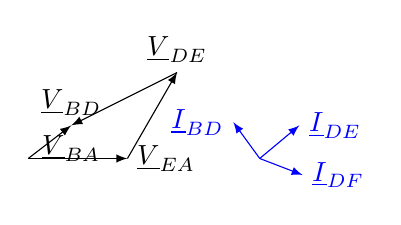
\begin{tikzpicture}[scale=.42,>=latex]
 \draw[->] (0,0)--(3,0) node[right]{$\underline V_{EA}$};
 \draw[->] (3,0)--(4.5,2.6) node[above]{$\underline V_{DE}$};
 \draw[->] (4.5,2.6)--(1.3,1.0) node[above]{$\underline V_{BD}$};
 \draw[->] (0,0)--(1.3,1.0) node[below]{$\underline V_{BA}$};
 \draw[->,blue] (7,0)--(8.2,1.0) node[right]{$\underline I_{DE}$};
 \draw[->,blue] (7,0)--(8.3,-.5) node[right]{$\underline I_{DF}$};
 \draw[->,blue] (7,0)--(6.2,1.1) node[left]{$\underline I_{BD}$};
\end{tikzpicture}
\caption{Fasordiagramma oefening 1. Spanningen: $1$~cm $=2$~V; stromen: $1$~cm $=0{,}5$~A.}
\end{figure}\FloatBarrier
\end{oefenblok}

\textbf{Opgave (foto-opgave 2): twee driefasige lasten.}
Een net heeft $V_L=240$~V. Een last $\underline{Z}_1$ hangt tussen $b$ en $c$ met
$S_1=80$~kVA en $\mathrm{pf}=0{,}9$ inductief. Een evenwichtige sterlast heeft
$S_Y=200$~kVA en dezelfde arbeidsfactor.
\begin{oefenblok}[Uitwerking]
Voor beide lasten is $\varphi=\arccos(0{,}9)=25{,}842^\circ$. De sterlast geeft:
\[
I_Y=\frac{200\cdot10^3}{\sqrt3\,240}=481{,}1\ \text{A}.
\]
Neem $\underline{V}_{ab}=240\angle0^\circ$~V. Dan:
\[
\underline{I}_{aY}=481{,}1\angle-55{,}84^\circ,\quad
\underline{I}_{bY}=481{,}1\angle-175{,}84^\circ,\quad
\underline{I}_{cY}=481{,}1\angle64{,}16^\circ\ \text{A}.
\]
De losse takstroom is
\[
\underline{I}_{bc}=\frac{80\,000}{240}\angle(-120^\circ-25{,}842^\circ)
=333{,}3\angle-145{,}84^\circ\ \text{A}.
\]
Met KCL:
\[
\boxed{\underline{I}_a=481{,}1\angle-55{,}84^\circ\ \text{A}},\quad
\boxed{\underline{I}_b=787{,}6\angle-163{,}63^\circ\ \text{A}},\quad
\boxed{\underline{I}_c=787{,}6\angle51{,}94^\circ\ \text{A}}.
\]
met: de losse stroom wordt bij lijn $b$ opgeteld en van lijn $c$ afgetrokken.
Controleer $\underline{I}_a+\underline{I}_b+\underline{I}_c=0$. Teken spanningen op
schaal $1$~cm $=50$~V en stromen op schaal $1$~cm $=200$~A.
\begin{figure}[H]\centering
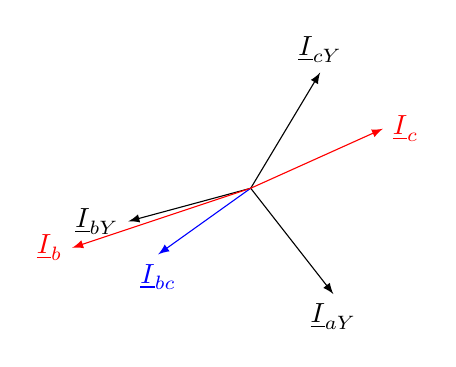
\begin{tikzpicture}[scale=.42,>=latex]
 \draw[->] (0,0)--(2.5,-3.2) node[below]{$\underline I_{aY}$};
 \draw[->] (0,0)--(-3.7,-1.0) node[left]{$\underline I_{bY}$};
 \draw[->] (0,0)--(2.1,3.5) node[above]{$\underline I_{cY}$};
 \draw[->,blue] (0,0)--(-2.8,-2.0) node[below]{$\underline I_{bc}$};
 \draw[->,red] (0,0)--(-5.4,-1.8) node[left]{$\underline I_b$};
 \draw[->,red] (0,0)--(4.0,1.8) node[right]{$\underline I_c$};
\end{tikzpicture}
\caption{Fasordiagramma oefening 2. Spanningen: $1$~cm $=50$~V; stromen: $1$~cm $=200$~A.}
\end{figure}\FloatBarrier
\end{oefenblok}

\textbf{Opgave (foto-opgave 3): arbeidsfactorcorrectie.}
Een bron van $100$~V bij $20$~Hz voedt $(3+j2)\,\Omega$ in serie met
$(5+j2)\parallel(3-j)\,\Omega$.
\begin{oefenblok}[Uitwerking]
\[
\underline{Z}_p=\frac{(5+j2)(3-j)}{8+j}=2{,}108-j0{,}138\ \Omega
\]
met: $\underline{Z}_p$ = equivalente parallelimpedantie. Dus:
\[
\underline{Z}_{tot}=5{,}108+j1{,}862=5{,}436\angle20{,}02^\circ\ \Omega.
\]
\[
\underline{I}=\frac{100}{\underline{Z}_{tot}}=17{,}283-j6{,}299\ \text{A},\quad
\underline{S}=100\underline{I}^{*}=1728{,}3+j629{,}9\ \text{VA}.
\]
De arbeidsfactor is $\boxed{0{,}940\ \text{inductief}}$. Voor $0{,}95$:
\[
\begin{aligned}
\varphi_2&=\arccos(0{,}95)=18{,}195^\circ,\\
|Q_C|&=P\left(\tan20{,}02^\circ-\tan18{,}195^\circ\right)\\
&=1728{,}3(0{,}3647-0{,}3289)=61{,}8\ \text{VAr}.
\end{aligned}
\]
\[
\boxed{C=\frac{|Q_C|}{100^2\,2\pi20}=49{,}2\ \mu\text{F}}.
\]
Teken twee vermogensdriehoeken: dezelfde horizontale $P=1728$~W, eerst
$Q=629{,}9$~VAr en daarna $Q=629{,}9-61{,}8=568{,}1$~VAr.
\begin{figure}[H]\centering
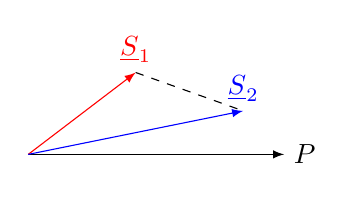
\begin{tikzpicture}[scale=.65,>=latex]
 \draw[->] (0,0)--(5,0) node[right]{$P$};
 \draw[->,red] (0,0)--(2.1,1.6) node[above]{$\underline S_1$};
 \draw[->,blue] (0,0)--(4.2,.85) node[above]{$\underline S_2$};
 \draw[dashed] (2.1,1.6)--(4.2,.85);
\end{tikzpicture}
\caption{Oude en gecorrigeerde vermogensdriehoek van oefening 3 (niet op fysieke lengteschaal).}
\end{figure}\FloatBarrier
\end{oefenblok}

\textbf{Opgave (foto-opgave 4): evenwichtige driehoeklast.}
Een $3\times174$~V-net bij $50$~Hz voedt een driehoek met per tak $R=30\,\Omega$ en
$L=31$~mH.
\begin{oefenblok}[Uitwerking]
\[
\underline{Z}_\Delta=30+j(2\pi50)(0{,}031)
=31{,}541\angle17{,}985^\circ\ \Omega.
\]
Met $\underline{V}_{AB}=174\angle0^\circ$~V:
\[
\underline{I}_{AB}=5{,}517\angle-17{,}985^\circ,\quad
\underline{I}_{BC}=5{,}517\angle-137{,}985^\circ,\quad
\underline{I}_{CA}=5{,}517\angle102{,}015^\circ\ \text{A}.
\]
De lijnstromen zijn verschillen in de hoekpunten:
\[
\boxed{\underline{I}_a=9{,}555\angle-47{,}985^\circ},\quad
\boxed{\underline{I}_b=9{,}555\angle-167{,}985^\circ},\quad
\boxed{\underline{I}_c=9{,}555\angle72{,}015^\circ\ \text{A}}.
\]
De takspanningen zijn $\underline{V}_{AB}=174\angle0^\circ$,
$\underline{V}_{BC}=174\angle-120^\circ$ en
$\underline{V}_{CA}=174\angle120^\circ$~V. Teken spanningen op schaal $1$~cm
$=50$~V en stromen op schaal $1$~cm $=2$~A.
\begin{figure}[H]\centering
\begin{tikzpicture}[scale=.42,>=latex]
 \draw[->] (0,0)--(3,0) node[right]{$\underline I_{AB}$};
 \draw[->] (0,0)--(-1.5,-2.6) node[below]{$\underline I_{BC}$};
 \draw[->] (0,0)--(-1.5,2.6) node[above]{$\underline I_{CA}$};
 \draw[->,red] (6,0)--(8.3,-2.0) node[right]{$\underline I_a$};
 \draw[->,red] (6,0)--(2.5,-1.1) node[left]{$\underline I_b$};
 \draw[->,red] (6,0)--(7.3,2.8) node[right]{$\underline I_c$};
\end{tikzpicture}
\caption{Fasordiagramma oefening 4. Spanningen: $1$~cm $=50$~V; stromen: $1$~cm $=2$~A.}
\end{figure}\FloatBarrier
\end{oefenblok}

\textbf{Opgave (foto-opgave 5): brug met twee bronnen.}
Gebruik de bronnen $8\angle30^\circ$~V en $1\angle90^\circ$~A en impedanties
$-2j$, $4j$, $2\,\Omega$, $2j$ en $-j\,\Omega$.
\begin{oefenblok}[Knooppuntanalyse]
Neem $N$ als referentie. Dan is $\underline{V}_D=8\angle30^\circ$~V. De KCL-vergelijkingen:
\[
\frac{V_A-V_D}{2}+\frac{V_A}{-j}+\frac{V_A-V_B}{j2}=0,\qquad
\frac{V_B-V_A}{j2}+\frac{V_B-V_D}{j2}-1\angle90^\circ=0.
\]
Oplossen geeft $\underline{V}_A=3{,}46-j3{,}65$~V en
$\underline{V}_B=4{,}19+j0{,}18$~V. De gevraagde stroom:
\[
\boxed{\underline{I}=\frac{\underline{V}_A}{-j}=5{,}03\angle43{,}5^\circ\ \text{A}}.
\]
Verder:
\[
\underline{I}_3=4{,}20\angle65{,}6^\circ,\quad
\underline{I}_4=1{,}95\angle169^\circ,\quad
\underline{I}_5=2{,}35\angle-35{,}6^\circ\ \text{A}.
\]
met: $\underline{I}_3$ door $2\,\Omega$, $\underline{I}_4$ door $j2\,\Omega$ en
$\underline{I}_5$ door de bovenste seriecombinatie. Teken de knoopspanningen vanuit
$N$ op schaal $1$~cm $=2$~V en de stromen als waaier op schaal $1$~cm $=1$~A.
\begin{figure}[H]\centering
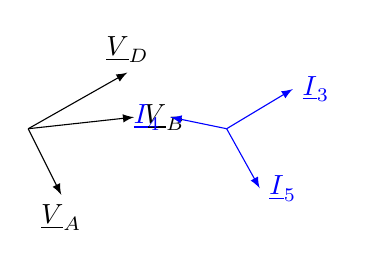
\begin{tikzpicture}[scale=.42,>=latex]
 \draw[->] (0,0)--(3,1.7) node[above]{$\underline V_D$};
 \draw[->] (0,0)--(1.0,-2.0) node[below]{$\underline V_A$};
 \draw[->] (0,0)--(3.2,.35) node[right]{$\underline V_B$};
 \draw[->,blue] (6,0)--(8,1.2) node[right]{$\underline I_3$};
 \draw[->,blue] (6,0)--(4.3,.35) node[left]{$\underline I_4$};
 \draw[->,blue] (6,0)--(7,-1.8) node[right]{$\underline I_5$};
\end{tikzpicture}
\caption{Fasordiagramma oefening 5. Spanningen: $1$~cm $=2$~V; stromen: $1$~cm $=1$~A.}
\end{figure}\FloatBarrier
\end{oefenblok}


\newpage
\thispagestyle{empty}
\vspace*{\fill}

\begin{center}
    \itshape\Huge
    Veel succes met de examens!
    \par\vspace{1cm}
    \normalfont\Large
    --- Ruben Ryckaert
\end{center}

\vspace{3cm}

\begin{quote}
    \centering
    \itshape\Large
    “Electricity is really just organized lightning.”
    \par\vspace{0.5cm}
    \textup{--- George Carlin}
\end{quote}

\end{document}
